\documentclass[12pt]{article}
 
\usepackage[margin=1in]{geometry}
\usepackage[font=small,labelfont=bf]{caption}
%\usepackage{graphicx}
\usepackage[draft]{graphicx}
\usepackage{amsmath, amsthm, amssymb, bm, enumitem, nicefrac, float, booktabs, adjustbox, subcaption, fancyhdr, makecell, titlesec, dsfont, epigraph}
\PassOptionsToPackage{hyphens}{url}\usepackage{hyperref}

\newcommand{\N}{\mathbb{N}}
\newcommand{\Z}{\mathbb{Z}}
\DeclareMathOperator*{\argmax}{argmax}
%\DeclareMathOperator*{\argmin}{argmin}
\newcommand{\argmin}{\mathop{\mathrm{argmin}}} 
\setcounter{MaxMatrixCols}{20}


\pagestyle{fancy}
\fancyhead{}
\setlength{\headheight}{15pt}
\setlength{\emergencystretch}{2pt} 
\fancyfoot{}
\fancyhead[L]{\slshape{Daily Fantasy Football}}
\fancyhead[R]{\slshape J.R. Becker \& J. St. Clair}
\fancyfoot[C]{\thepage}


\begin{document}

\begin{titlepage}
	\begin{center}
	\vspace*{4cm}
	\huge{\textbf{Daily Fantasy Football}}\\[2cm]
	\Large{By\\[2mm] Jason R. Becker \& Jack St. Clair}\\[2cm]
	\large{A report submitted as an independent study project for the\\
		Master of Financial Engineering Program at the\\
		 University of California, Berkeley}\\[1cm]	
	\Large{Spring 2019}\\[2cm]
	
\includegraphics[scale=0.3]{../figures/fantasy_logo}
	\vfill
	\line(1,0){400}
	\end{center}
\end{titlepage}


\section{Introduction}
TODO



\pagebreak
\section{Data Summary}
TODO


\subsection{Data Collection}
\begin{table}[H]
\caption{Data collected from each source.}
\small
\label{sources}
\centering
\begin{tabular}{lcc}
	\toprule
	Source        &  Full Season              &  Weekly \\
	\midrule
	CBS           &  QB, RB, WR, TE, DST, K   &   QB, RB, WR, TE, DST, K \\
	ESPN          &  QB, RB, WR, TE, DST, K   &   QB, RB, WR, TE, DST, K \\
	FantasyPros   &  QB, RB, WR, TE, DST, K   &   QB, RB, WR, TE, DST, K \\
	FFToday       &  QB, RB, WR, TE, DST, K   &   QB, RB, WR, TE, K \\
	NFL.com       &  QB, RB, WR, TE, DST, K   &   QB, RB, WR, TE, DST, K \\
	RTSports      &  QB, RB, WR, TE, DST, K   &    {} \\
	Yahoo         &  {}                       &   QB, RB, WR, TE, DST, K \\
	\midrule
	DraftKings    &  {}                       &   QB, RB, WR, TE, DST \\
 	FanDuel       &  {}                       &   QB, RB, WR, TE, DST \\
	\bottomrule
\end{tabular}
\end{table}

For the scope of this report, full season analysis will be neglected. However, the data has been collected, allowing for potential future work on full season projections which may prove useful for season long fantasy leagues. As daily fantasy websites such as DraftKings and FanDuel do not include kickers in possible lineups, kickers will also be neglected for the remainder of this report.\bigskip

For each position, a variety of stats are projected from the various sources. Due to lack of consistency between which stats are projected and which are not among the sources, stats were broken down into two categories. The first category we denote \textit{essential stats}, stats which are projected by most of the sources and are generally non-zero in value. The second category we denote \textit{nonessential stats}, stats which may not be projected by more than a couple sources and are generally 0 or near 0 in value. Table \ref{stats table} lists the essential and nonessential stats for each position.

\begin{table}[H]
\caption{Essential and nonessential stats for each position.}
\small
\label{stats table}
\centering
\begin{adjustbox}{width =\textwidth}
\begin{tabular}{lcc}
	\toprule
	Position        &  Essential Stats            &  Nonessential Stats \\
	\midrule
	QB   &  Pass Yds, Pass TD, Pass Int, Rush Yds, Rush TD,   &   Receptions, Rec Yds, Rec TD, 2PT\\
	RB   &  Rush Yds, Rush TD, Receptions, Rec Yds, Rec TD   &   Pass Yds, Pass TD, Pass Int, 2PT \\
	WR   &  Rush Yds, Rush TD, Receptions, Rec Yds, Rec TD   &   Pass Yds, Pass TD, Pass Int, 2PT \\
	TE   &  Receptions, Rec Yds, Rec TD    &   Pass Yds, Pass TD, Pass Int, Rush Yds, Rush TD, 2PT\\
	DST  &  PA, YdA, TD, Sack, Int, Fum Rec & Saf, Blk \\
	\bottomrule
\end{tabular}
\end{adjustbox}
\end{table}


\subsection{Missing Data}

Among data collection sources, the number of players with projections was not consistent, and in many cases projections are only provided from 4 or 5 out of 6 sources for a particular player. The number of sources which provided projections for each essential stat, and the percentage of missing data are provided in Figure \ref{missing data}. Nonessential statistics are provided in the appendix. These instances were manually observed and found to not be restricted to backups, but often occur in prominent starting players (e.g., Drew Brees, Cam Newton). Since prominent players were affected, the players with missing projections could not be dropped, necessitating imputing of missing values.\bigskip


\begin{figure}[H]
  \centering
  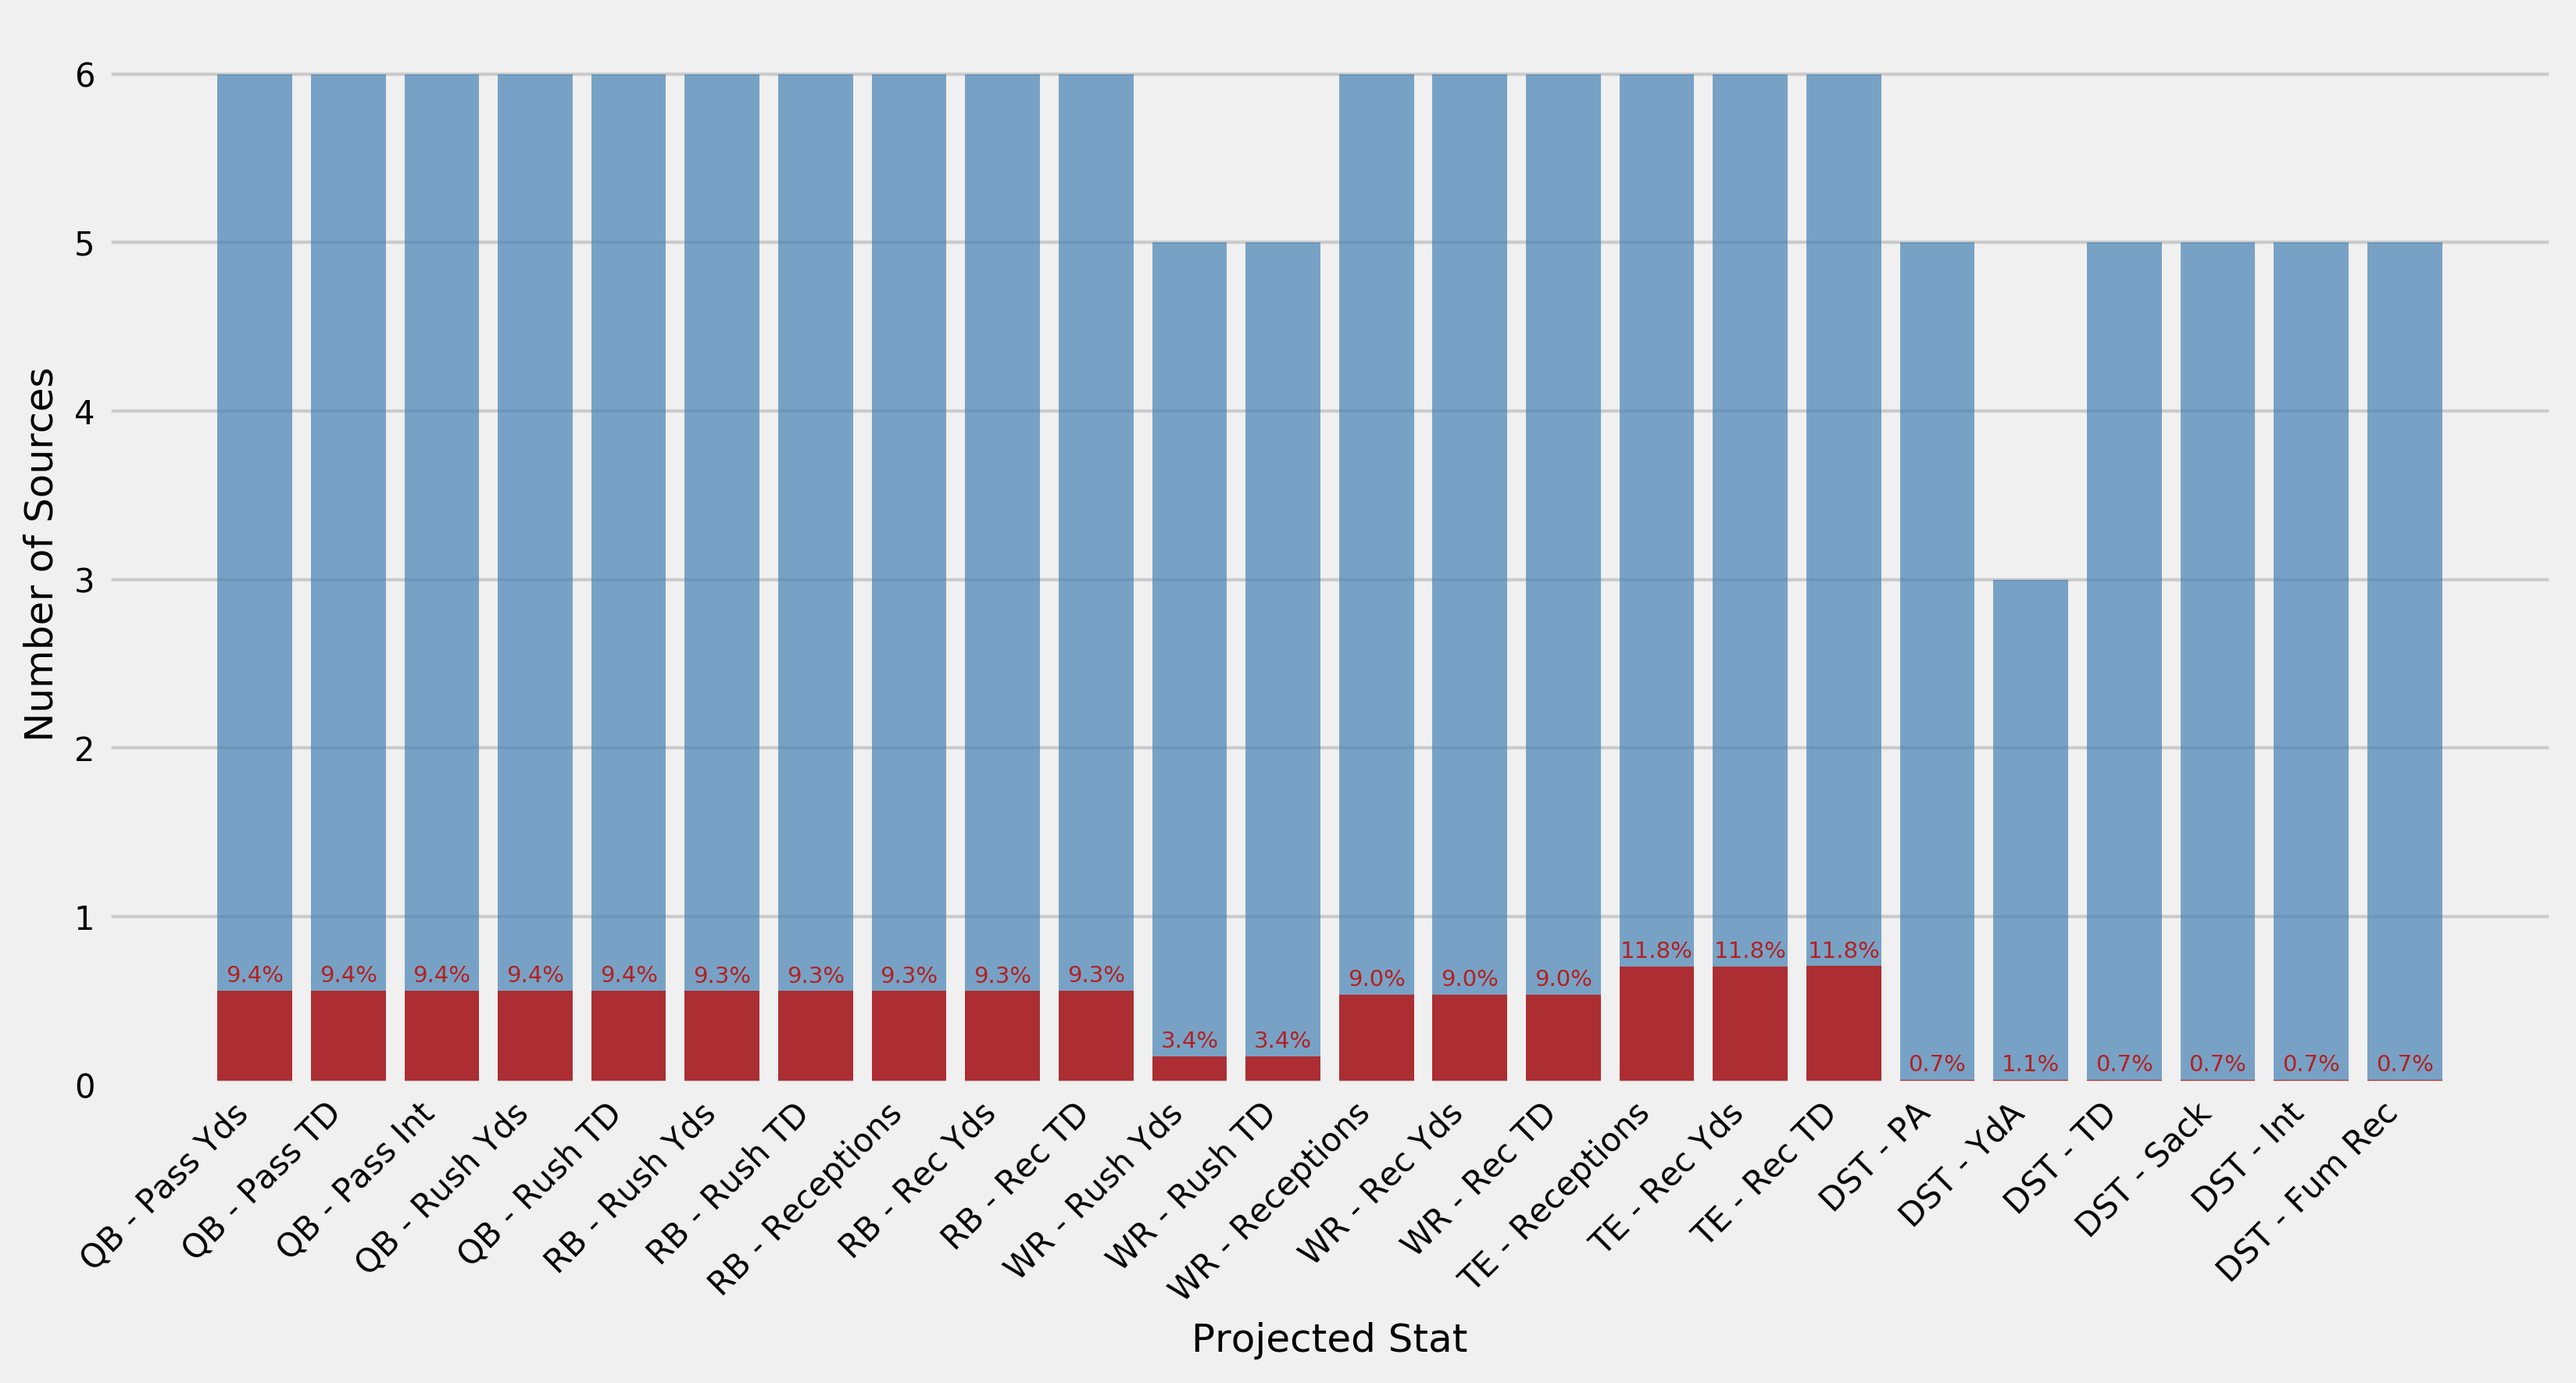
\includegraphics[width=0.95\textwidth]{../figures/missing_data}
  \caption{Number of sources collected for each essential stat (blue). Red indicates percentage of missing data for each respective stat.}
  \label{missing data}
\end{figure}

Several imputing methods were tested to find the optimal method for imputing missing projections. Imputing algorithms from the \texttt{fancyimpute} Python package were utilized to perform the imputing\cite{fancyimpute}. The simplest of these techniques as simply filling the projections from missing sources with the mean or median of the collected projections. Several more advanced methods were also studied. First, an iterative imputing method was used, where each source with missing values was first modeled as a function of all other sources using rows with full data, and these respective models were subsequently used to impute missing values for each source. Second, a K-nearest neighbors (KNN) approach was used, where each source is given a weight based on rows with all data observed. A matrix factorization approach was also studied which uses gradient descent to directly solve a factorization of the incomplete matrix into low-rank $U$ and $V$ matrices with L1 and L2 regularization respectively. Finally a soft impute method was studied which completes the matrix via soft thresholding singular value decompositions (SVD). Strictly using SVD was not possible due to the low number of sources (6) compared to the number of players which ranged from 32 for DST to upwards of 200 for WR. More information regarding each method and literature is available at \cite{fancyimpute}.\bigskip

In order to test which imputing method was best suited for the stat projection dataset, a raw matrix of all projected players for every week of the season was compiled for each stat. Players with 50\% or more sources missing were dropped, as these players were always either backups or players not expected to start, resulting in an incomplete matrix. Next, the percentage of missing data in the incomplete matrix for each respective stat was recorded, shown in Figure \ref{missing data}. All rows (players) with any missing values were subsequently removed, leaving a fully completed matrix for each stat. Elements in this completed matrix were then removed at random until the matrix had an equivalent missing data percentage as incomplete matrix. Each imputation method described above was then used to impute these missing values, with the mean average error (MAE) and root mean squared error (RMSE) recorded for the difference between the imputed matrix of each method and the complete matrix of true projection values. This process was repeated for 50 simulations in order to reduce potential variation from the random selection of missing elements. The resulting MAE and RMSE values for each imputing method of the essential stats is provided below. 


\begin{figure}[H]
  \centering
  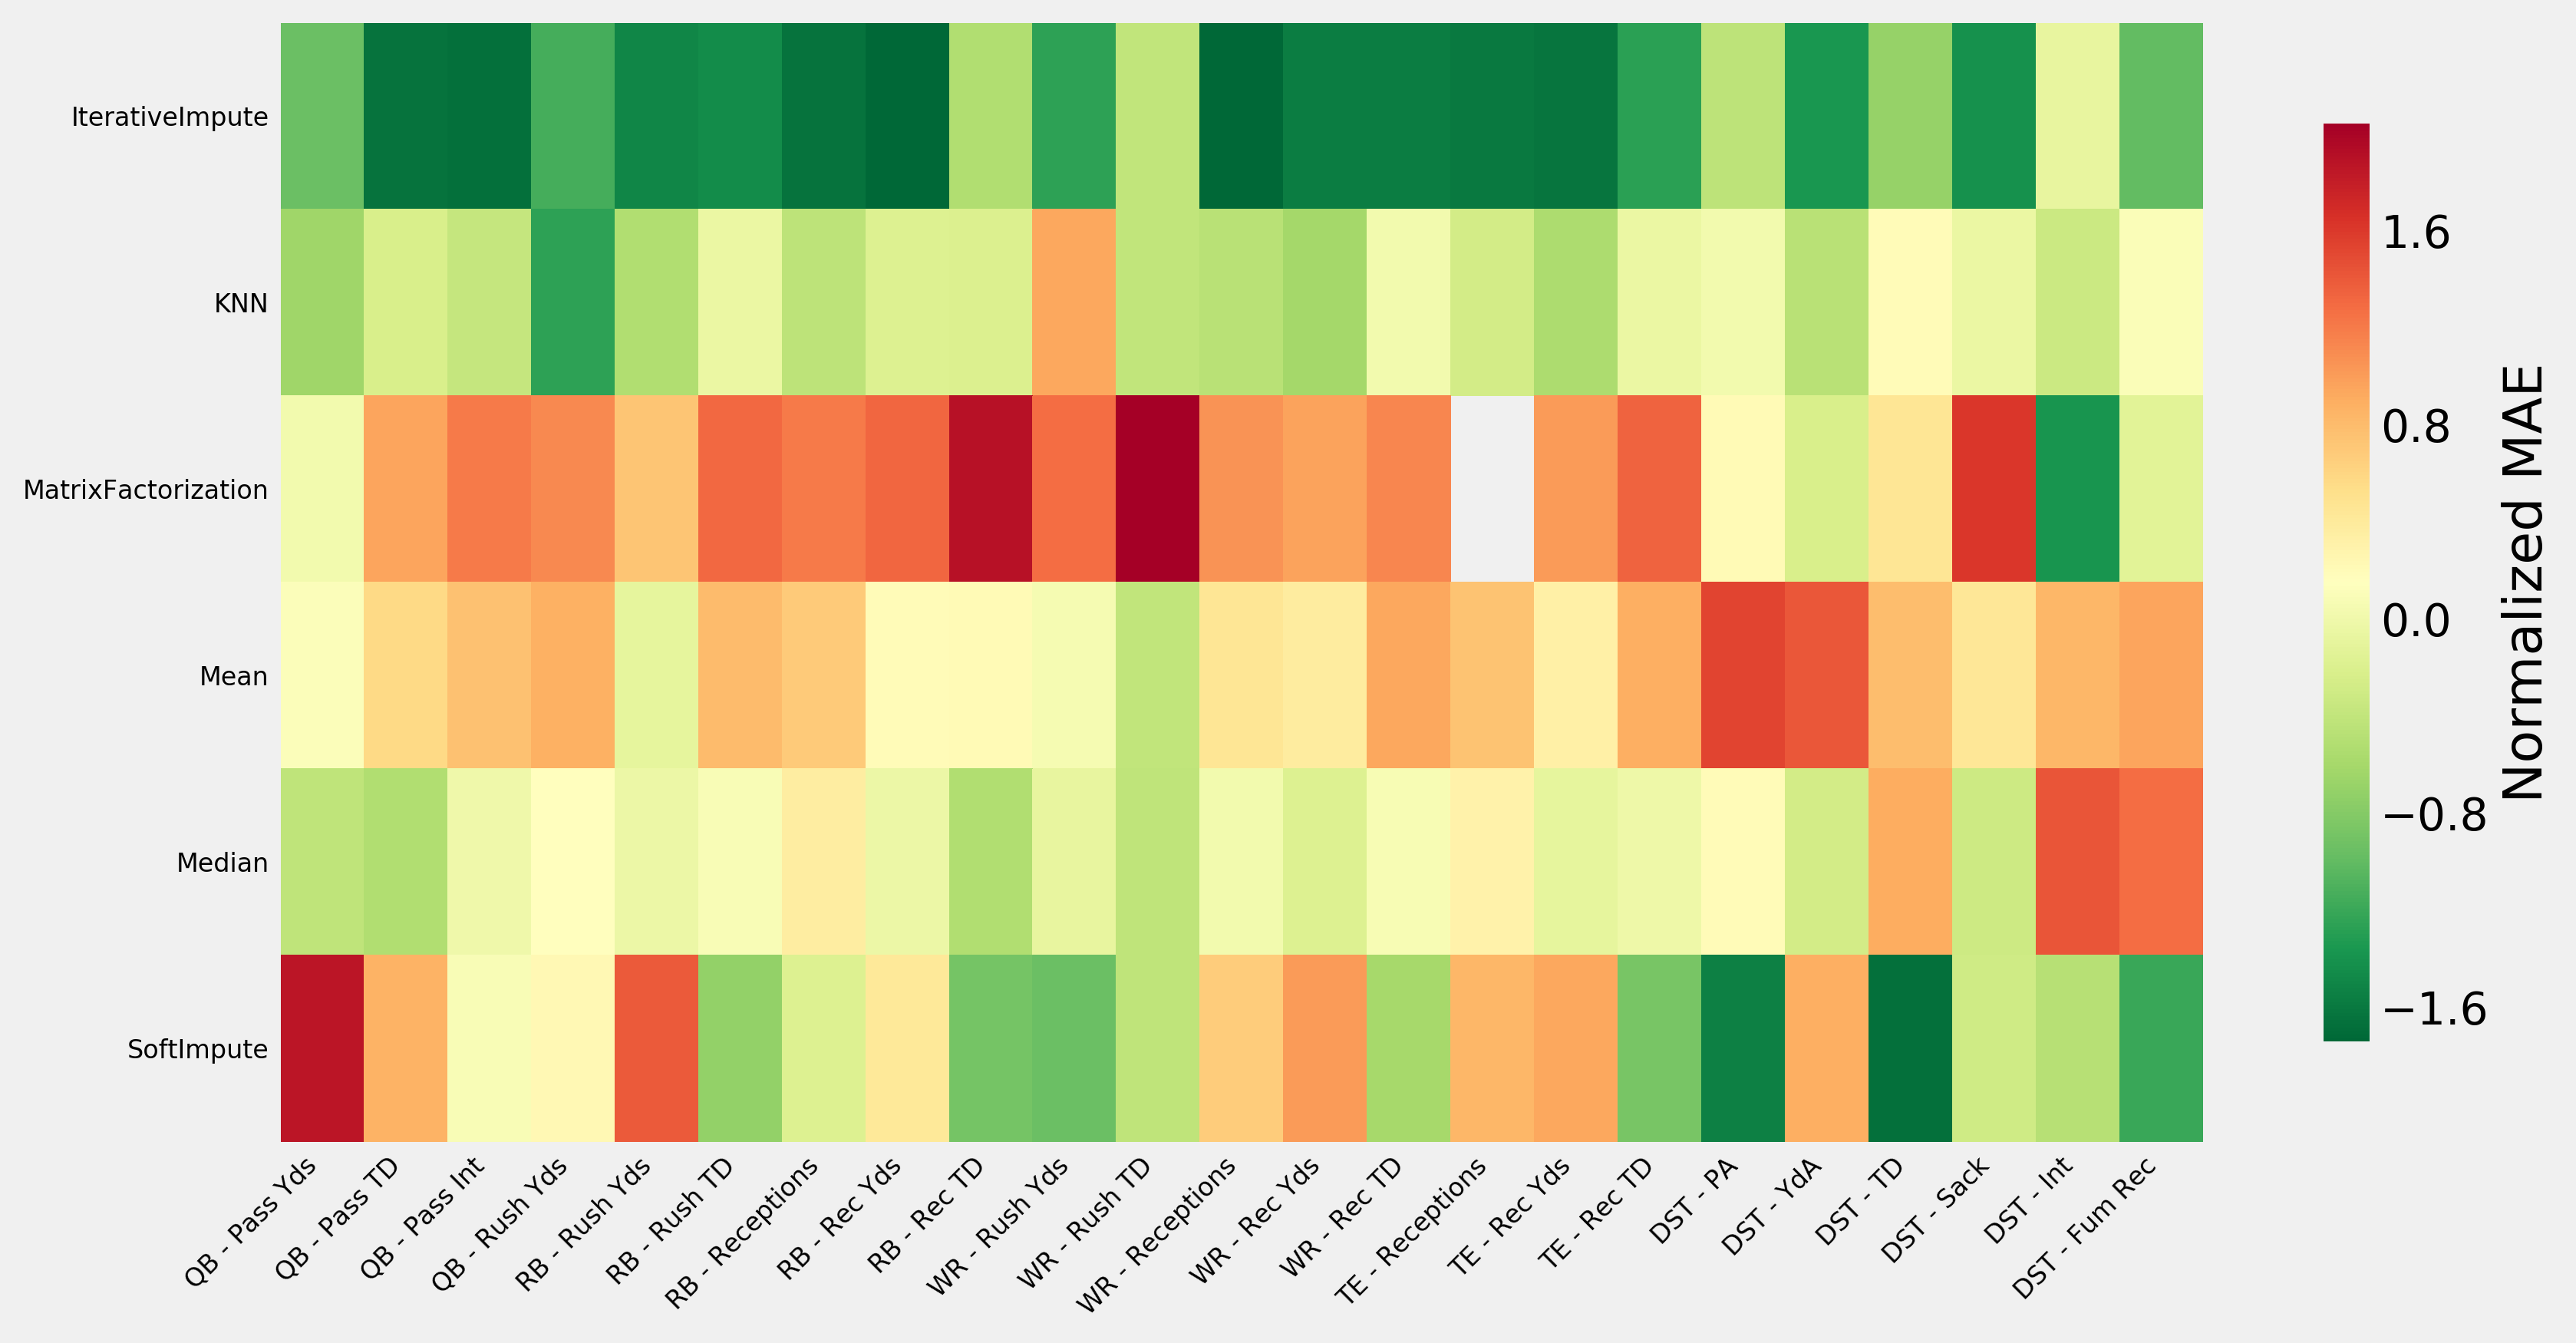
\includegraphics[width=0.95\textwidth]{../figures/impute_MAE}
  \caption{Normalized MAE of imputing methods for each essential stat.}
  \label{impute MAE}
\end{figure}

\begin{figure}[H]
  \centering
  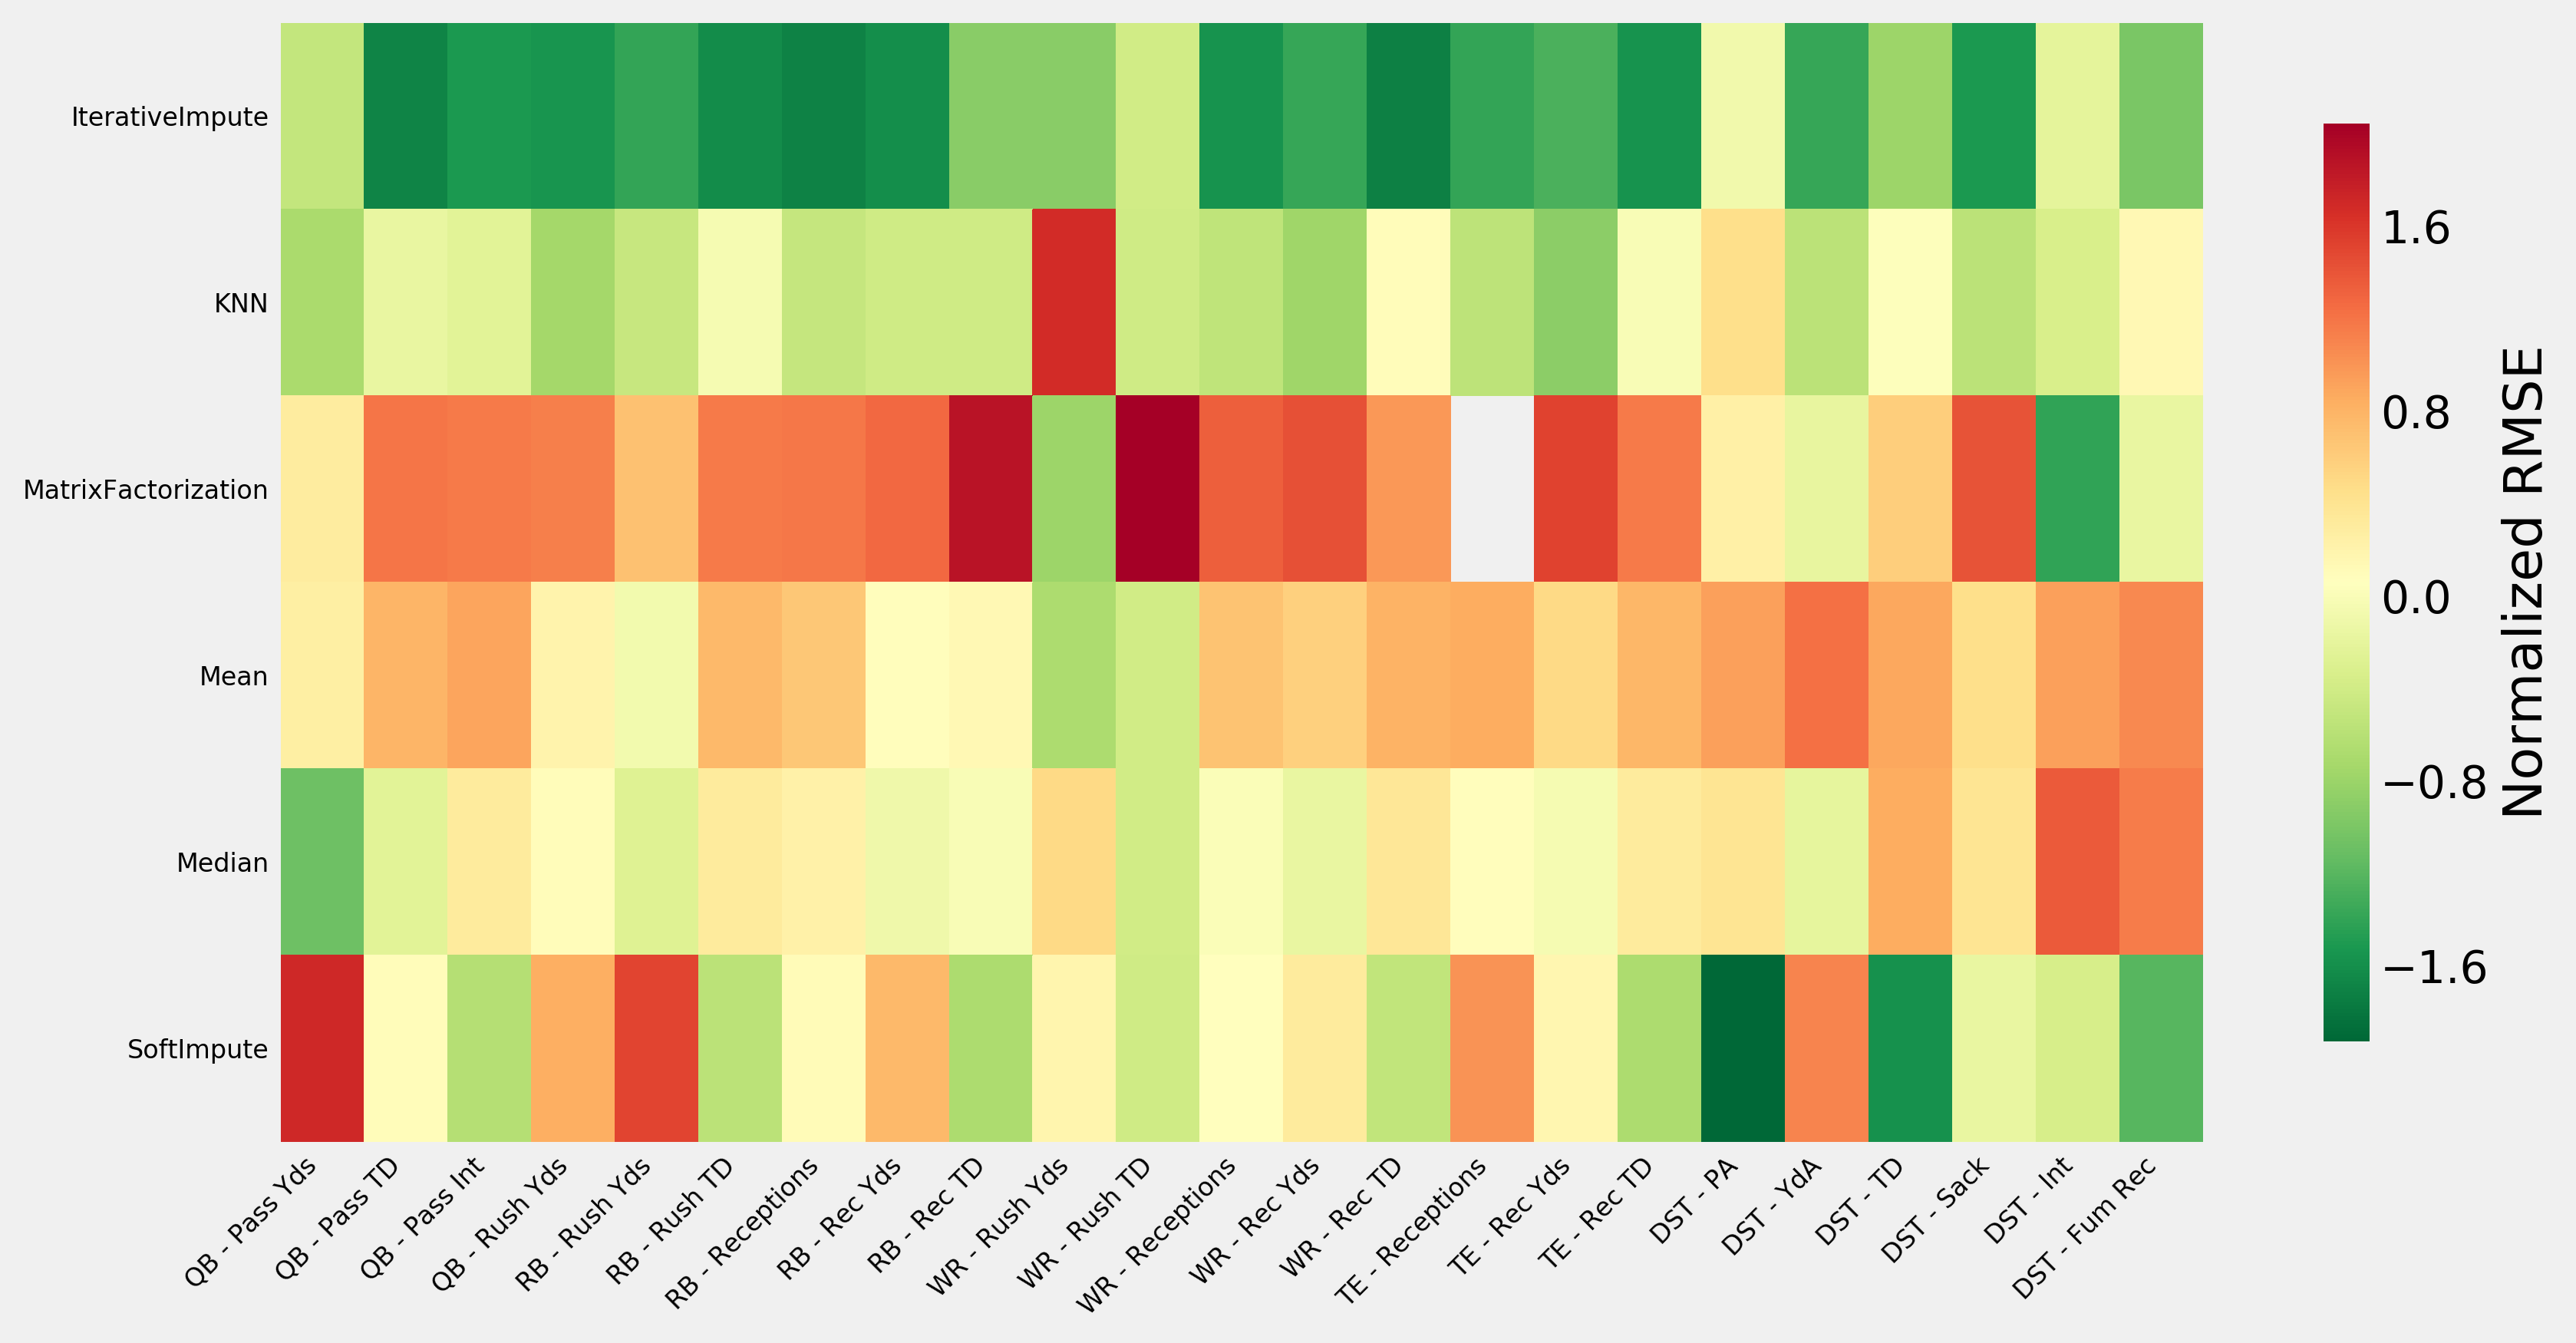
\includegraphics[width=0.95\textwidth]{../figures/impute_RMSE}
  \caption{Normalized RMSE of imputing methods for each essential stat.}
  \label{impute RMSE}
\end{figure}

Figures \ref{impute MAE} and \ref{impute RMSE} clearly indicate that the iterative imputing method provides the best estimates for missing values.  A comparison of imputing techniques for nonessential stats is provided in the appendix, where iterative imputing was again found to be optimal. Therefore iterative imputing was used to impute missing values for both essential and nonessential stats for the remainder of this study.

\subsection{Data Exploration}


\begin{figure}[H]
  \centering
  \begin{subfigure}[b]{0.450\textwidth}
    \centering
    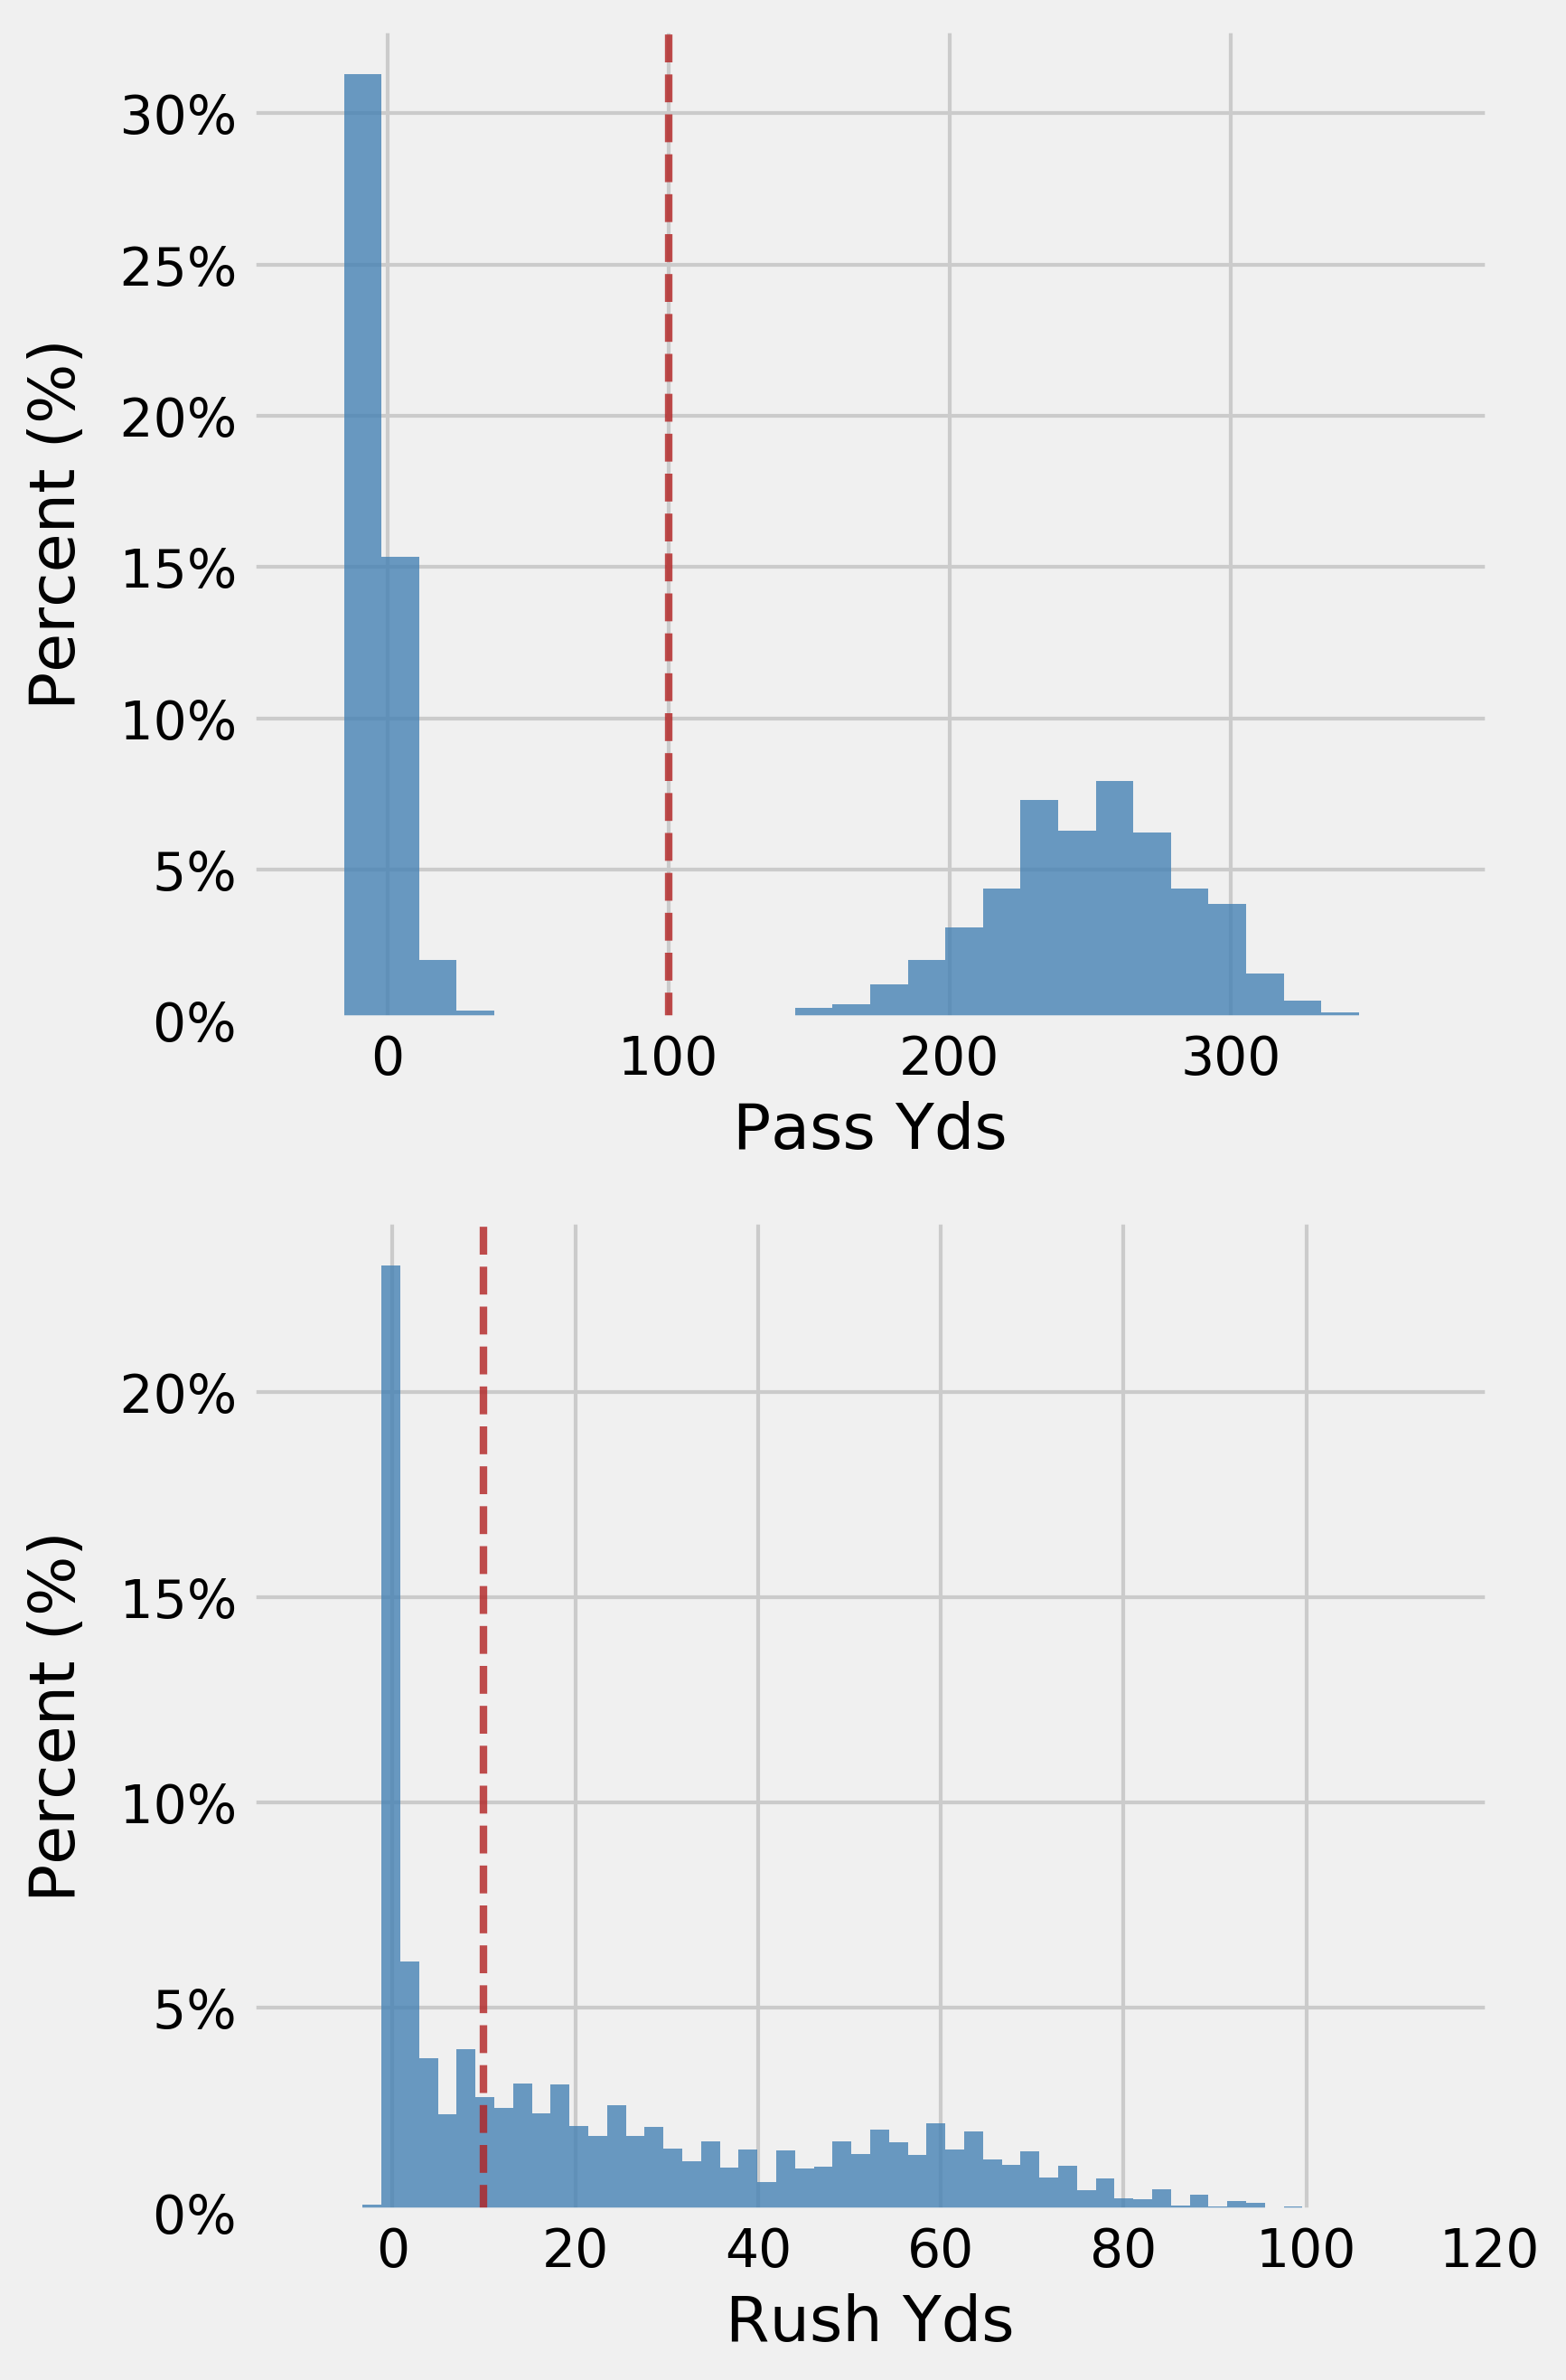
\includegraphics[width=1\textwidth]{../figures/no_theshold_example_hists}
    \caption{Raw histogram with threshold (red).}
  \end{subfigure}
  \hfill
  \begin{subfigure}[b]{0.450\textwidth}
    \centering
    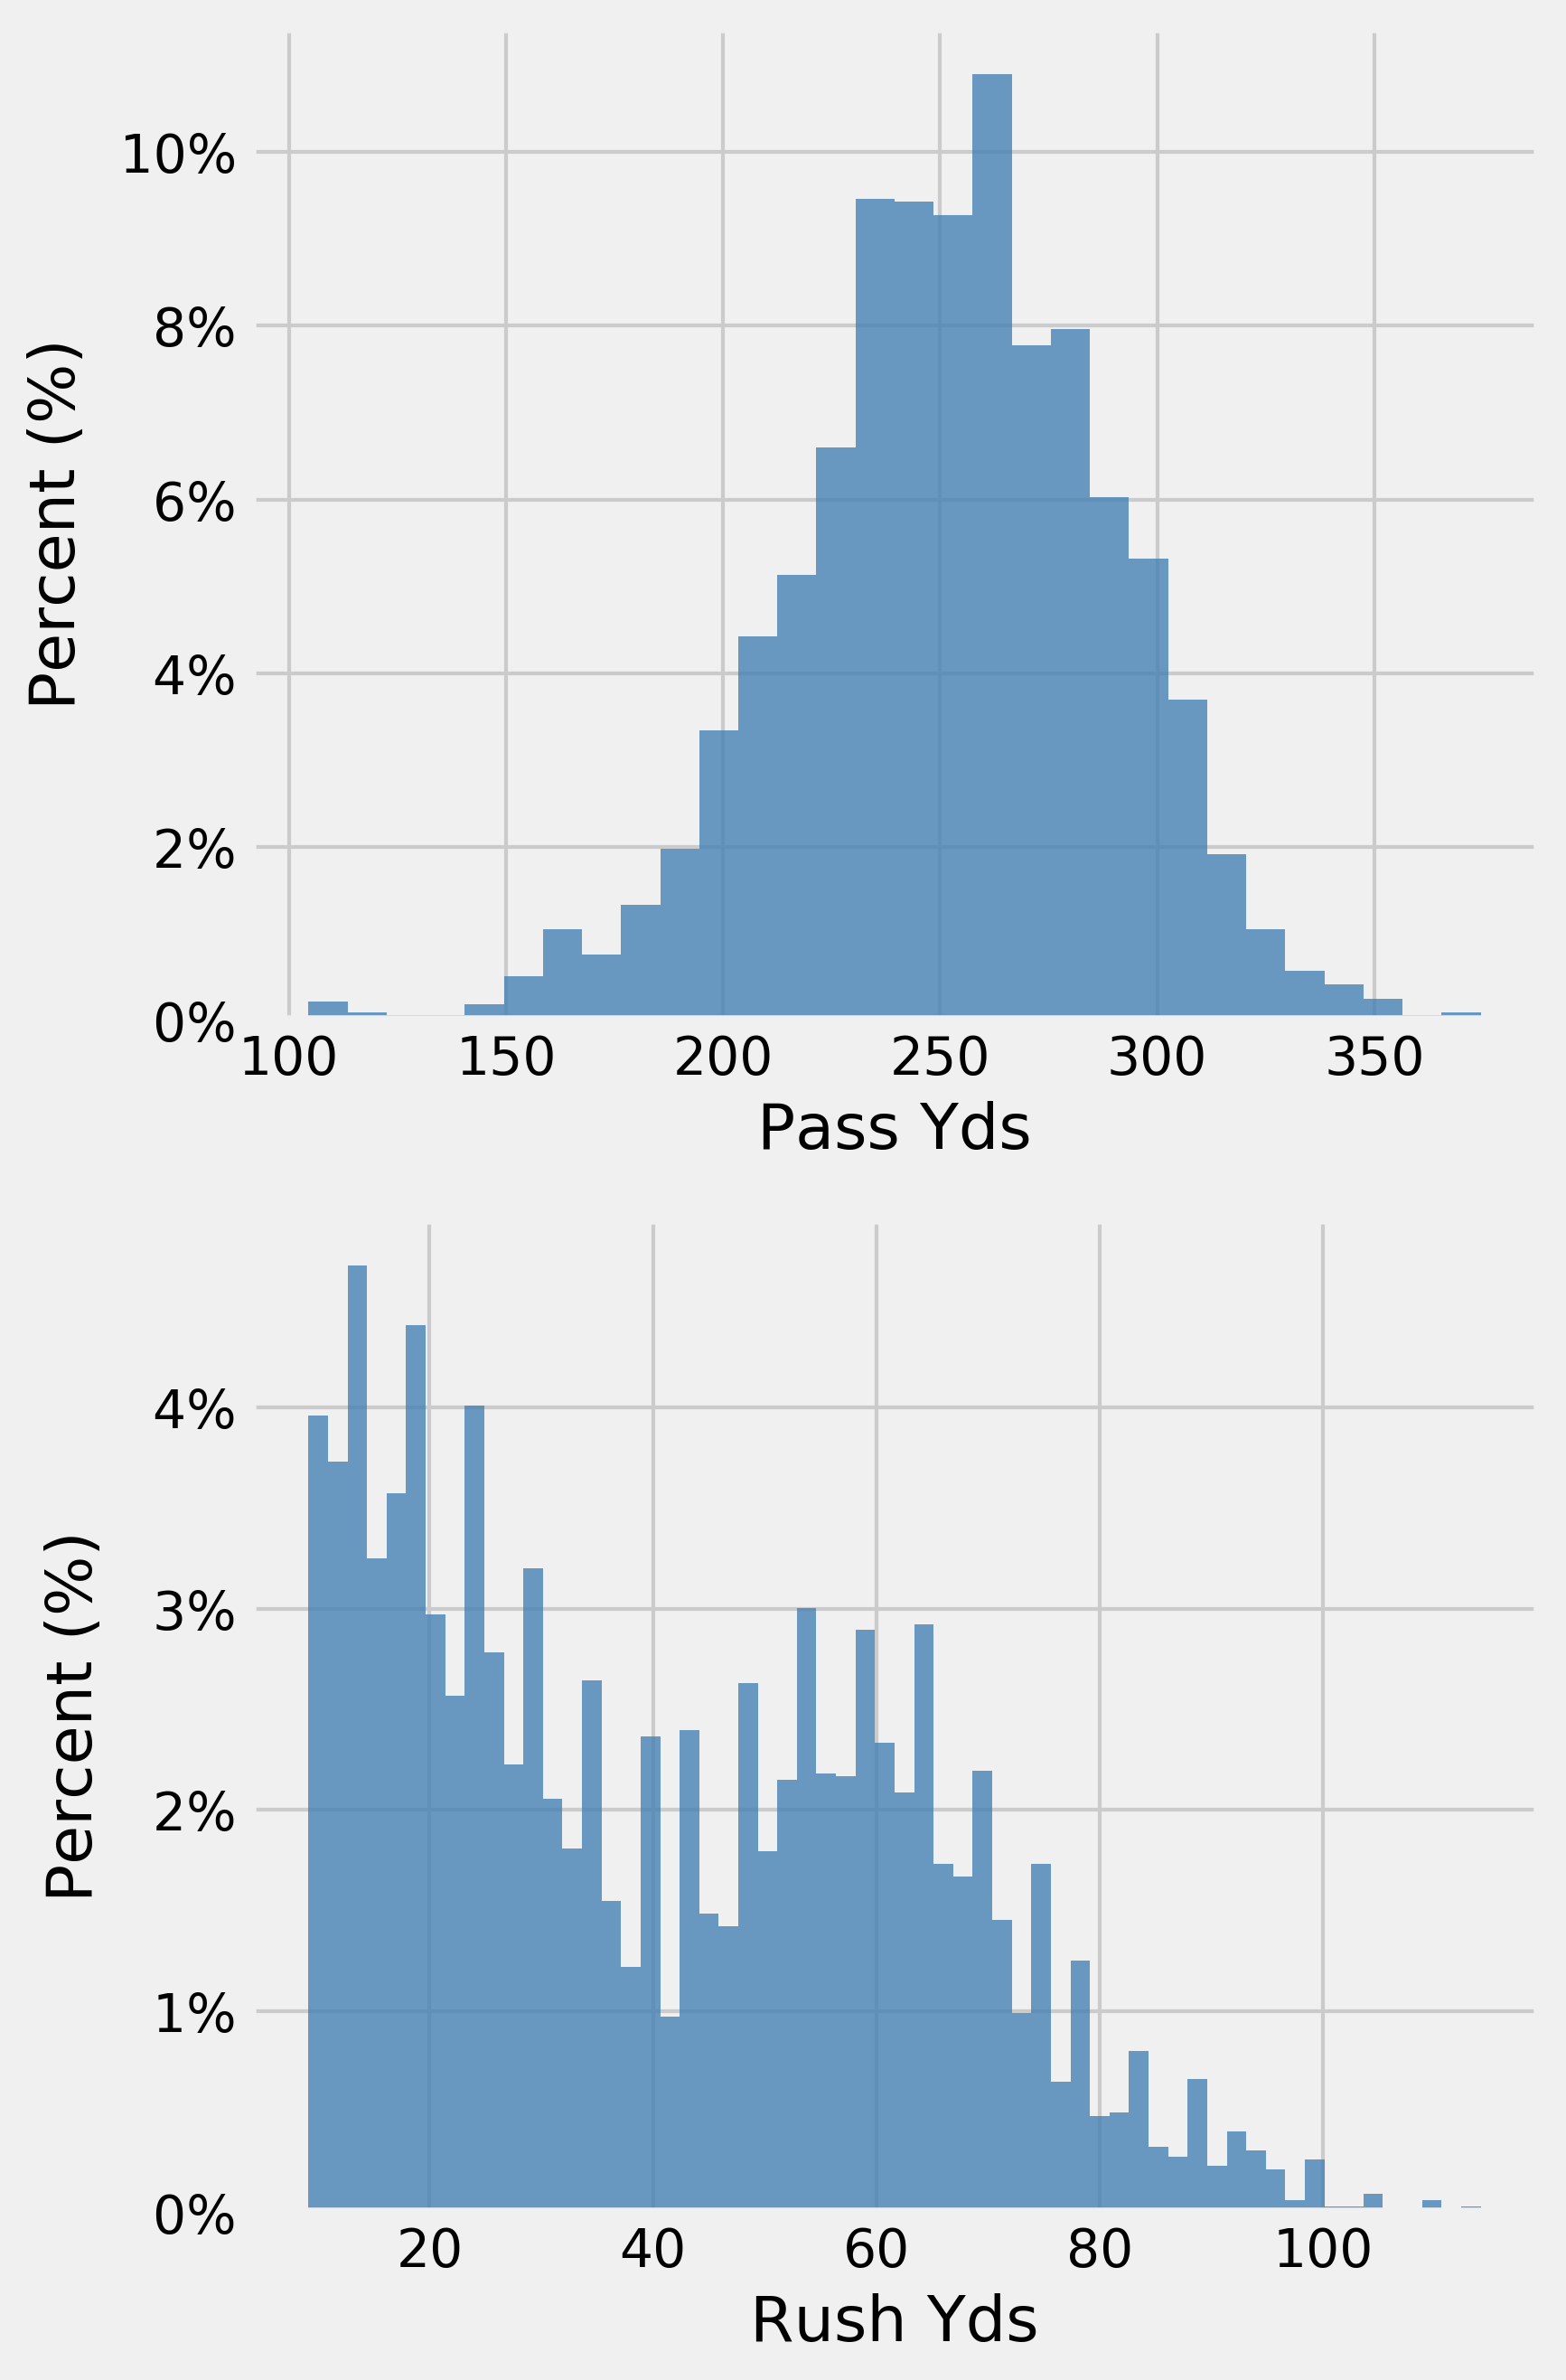
\includegraphics[width=1\textwidth]{../figures/no_theshold_example_hists_RB}
    \caption{Histogram above threshold.}
  \end{subfigure}
  \caption{Example raw and thresholded histograms for QB passing yards and RB rushing yards.}
\end{figure}


\pagebreak
\section{Methodology}
\subsection{Projections}
TODO
\subsection{Lineup Optimization}
Given optimal player projections, lineups must now be generated for competition at DraftKings and FanDuel. Both sites have the same lineup restrictions, only differing on their budget and point system (DraftKings is 50,000 budget and 1 pt per reception; FanDuel is 60,000 budget and is 0.5 pts per reception). As the goal is to score as many points as possible, projected points were maximized such that all lineup restrictions were met. \bigskip

In order to use convex optimization to solve for the optimal lineup, as opposed to brute-force solving for all possible combinations, we define the following problem: \begin{itemize}
	\item Let $N$ be the number of total players.
	\item Let $B$ be the salary budget for the contest.
	\item Let $w \in \mathbb{R}^{N}$ be a vector of player-weights, such that $w_i \in {0, 1}$.
	\item Let $P \in \mathbb{R}^{N}$ be a vector of projected points.
	\item Let $S \in \mathbb{R}^{N}$ be a vector of salaries.
	\item Let $D \in \mathbb{R}^{N \times 5}$ be a matrix containing the position of  each player, using dummy variables for each position. That is, $p_{i, j} \in {0, 1}$.
	\item Let $C \in \mathbb{R}^{N \times 32}$ be a matrix containing the team of each player, using dummy variables for each team. That is, $T_{i, j} \in {0, 1}$.
\end{itemize}
Then, we solve for the $w$ that solves:
\begin{equation*}
\begin{aligned}
& \underset{w}{\text{maximize}}
& & w^T \cdot P \\
& \text{subject to}
& & w^T \cdot S \leq B, \; \mathds{1} \cdot w = 9, \\
&&& (w^T \cdot D)_1 = 1, \\
&&& 2 \leq (w^T \cdot D)_2 \leq 3, \\
&&& 3 \leq (w^T \cdot D)_3 \leq 4, \\
&&& 1 \leq (w^T \cdot D)_4 \leq 2, \\
&&& (w^T \cdot D)_5 = 1, \\ 
&&& \max_i (w^T \cdot C)_i \leq 4 \\
\end{aligned}
\end{equation*}
where the subscripts $1,\ldots ,5$ on $(w^T \cdot D)$ correspond to the positions QB, RB, WR, TE, and Defense, respectively. These constraints ensure that each lineup follows the composition rules defined in each contest.

While this formulation worked perfectly when solving for the highest projected lineup, it failed when scaling to the solve for the highest $n$ projected lineups. As many contests allow for up to 150 lineup entries per person, this limitation must be solved for. Below in figure \ref{lineup times}, the exponential nature of the slowdown is shown.

\begin{figure}[H]
  \centering
  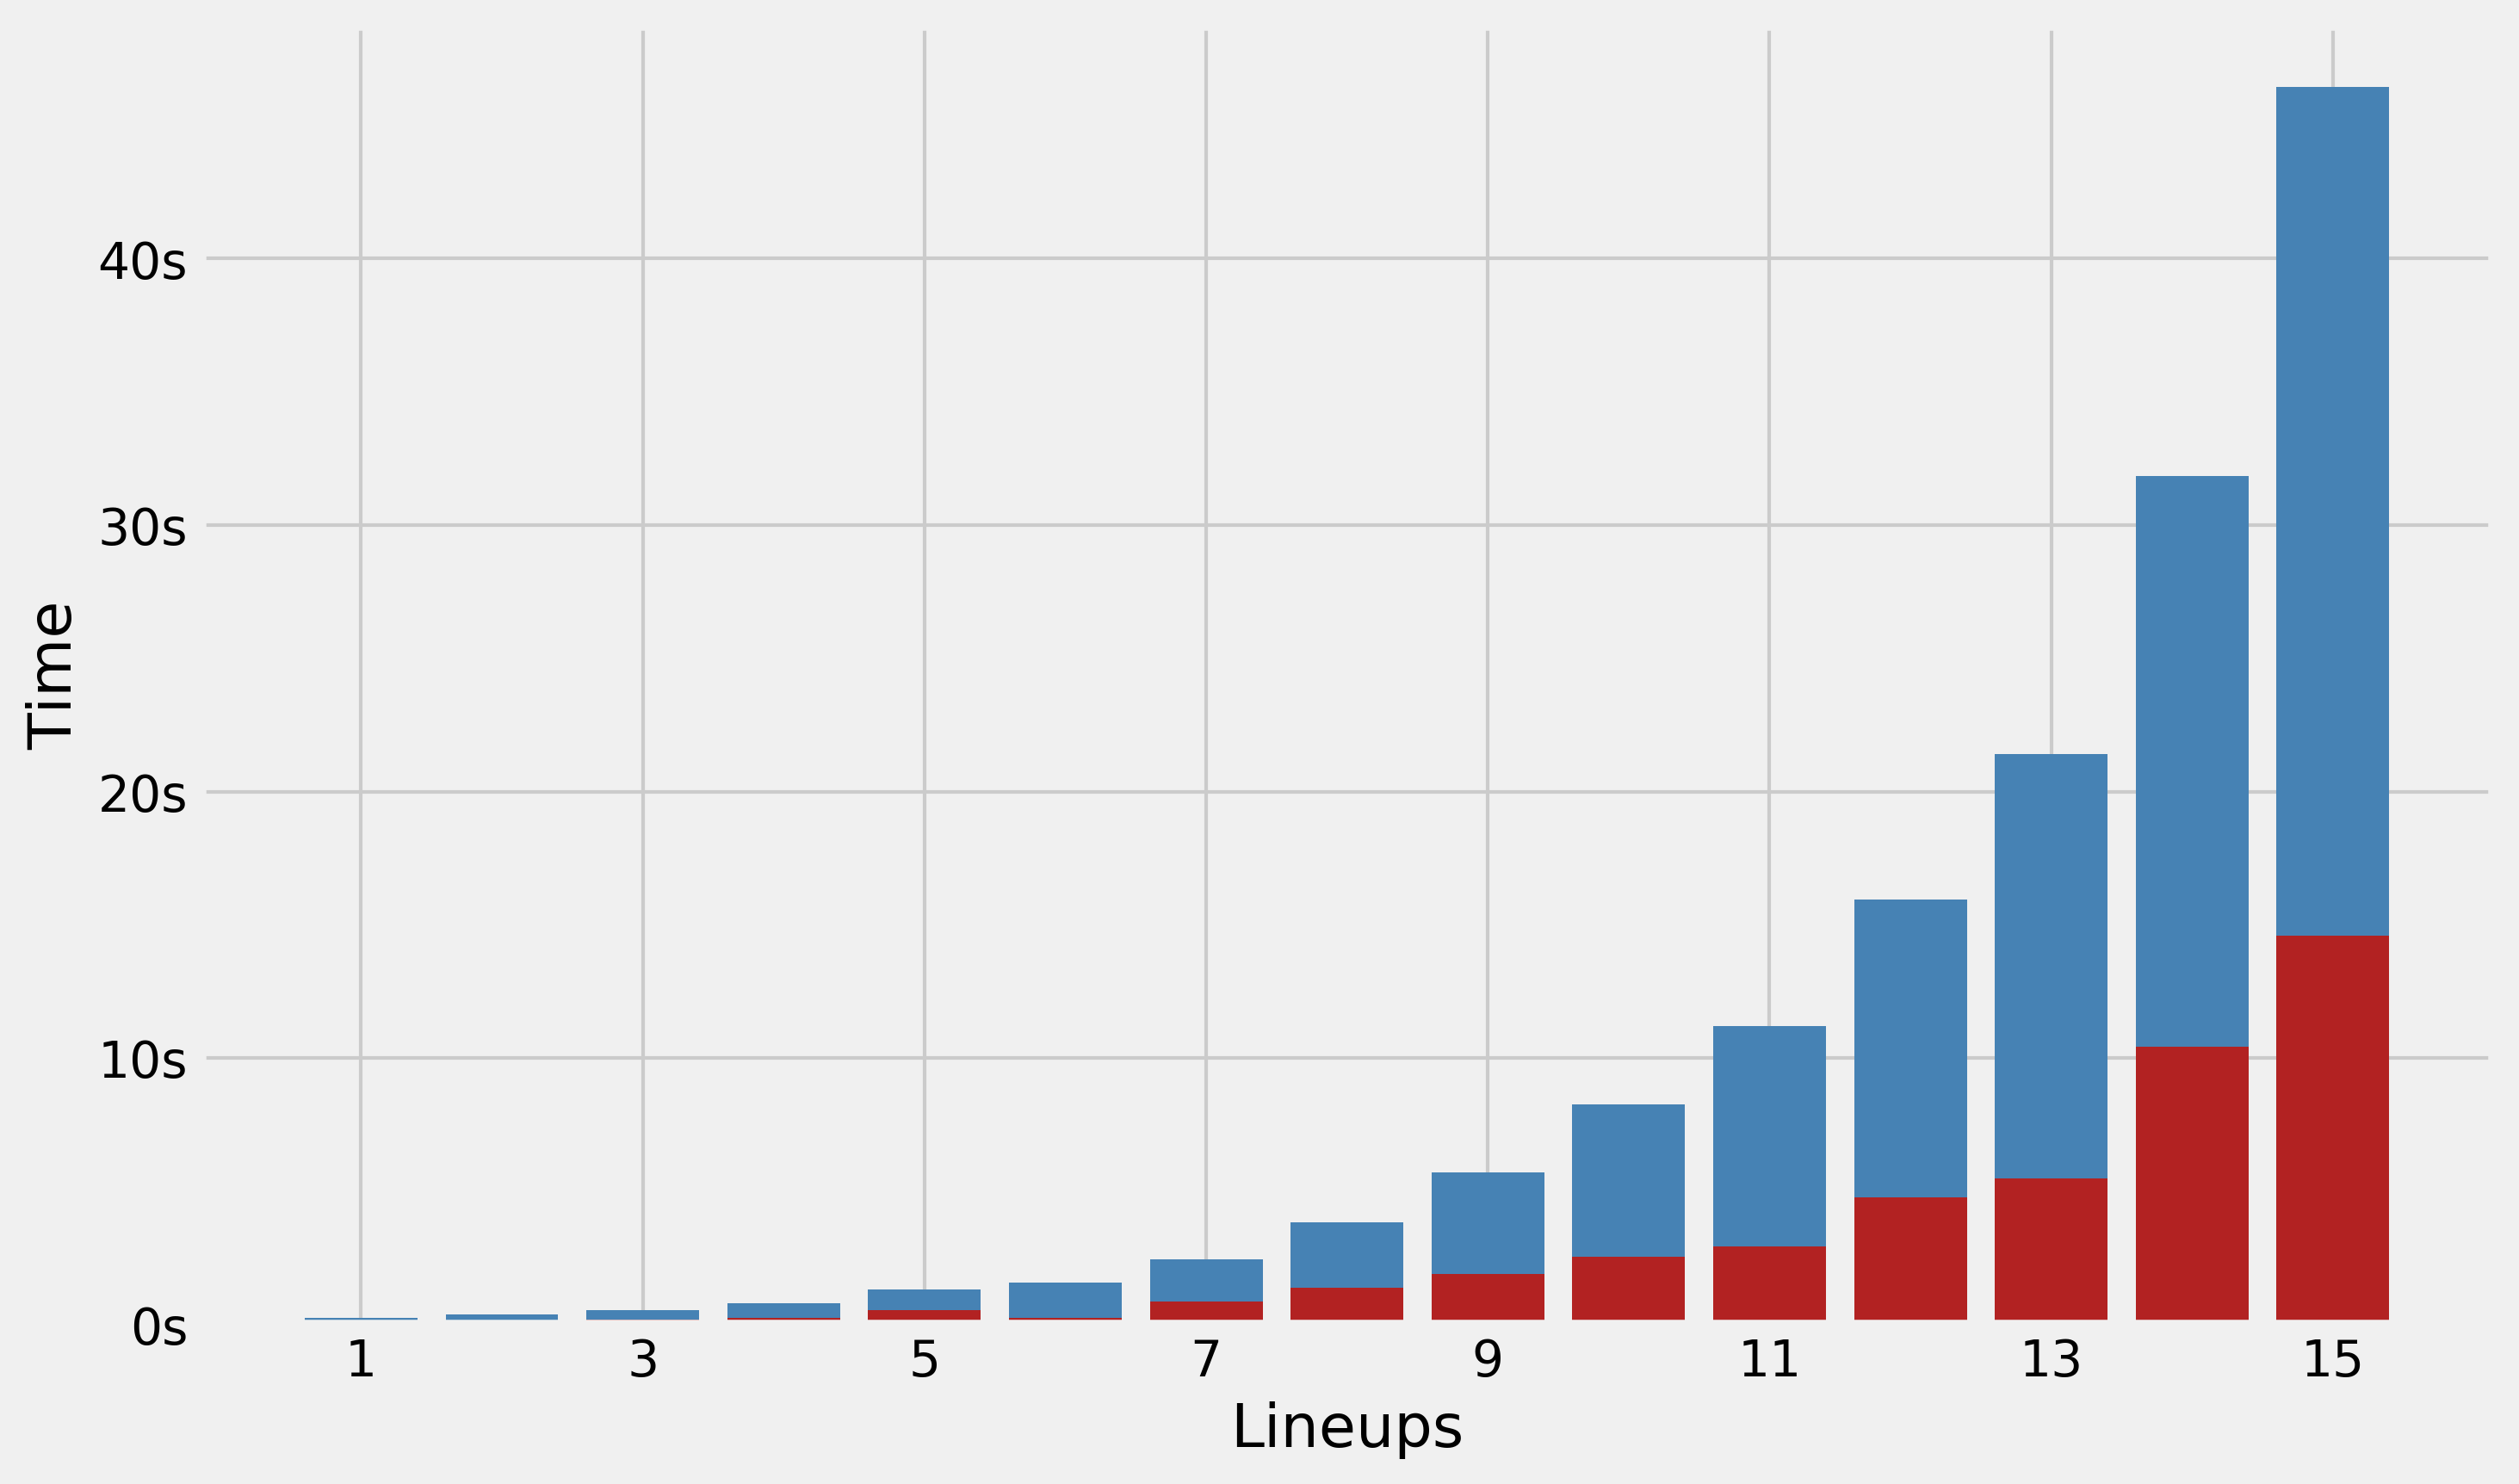
\includegraphics[width=0.95\textwidth]{../figures/time_per_lineup}
  \caption{Cumulative (in blue) and marginal (in red) time taken to generate lineups.}
  \label{lineup times}
\end{figure}

As a remedy for this problem, we implement a dropout-like system in which players are dropped from the available pool with probability $p$ (CITE). Thus, the probability that the best possible lineup gets chosen is equal to $(1-p)^9$. Below in Table \ref{probs_of_lineups}, these probabilities are shown for different values of $p$.

\begin{table}[H]
\caption{Probability of best lineup being selected for varying levels of dropout probability $p$.}
\label{probs_of_lineups}
\centering
\begin{tabular}{lcc}
\toprule
{} &     $p$ &  $\Pr$(Max)  \\
\midrule
{} &  0.00 &  1.00 \\
{} &  0.05 &  0.63 \\
{} &  0.10 &  0.39 \\
{} &  0.15 &  0.23 \\
{} &  0.20 &  0.13 \\
{} &  0.25 &  0.08 \\
{} &  0.30 &  0.04 \\
{} &  0.35 &  0.02 \\
{} &  0.40 &  0.01 \\
\bottomrule
\end{tabular}
\end{table}

Now of course, for what this approach gains in speed, it loses in precision. We have now introduced a non-zero probability that the best possible $n$ lineups will not be selected if we choose to generate exactly $n$ lineups, given the randomness of dropout. Using week 1 of 2018 as a test, 400 lineups were generated, and the first $n$ lineups generated are examined below in Figure \ref{lineups_vs_n}. Both the top 10 and top 150 lineups are studied.  

\begin{figure}[H]
  \centering
  \begin{subfigure}[b]{0.80\textwidth}
    \centering
    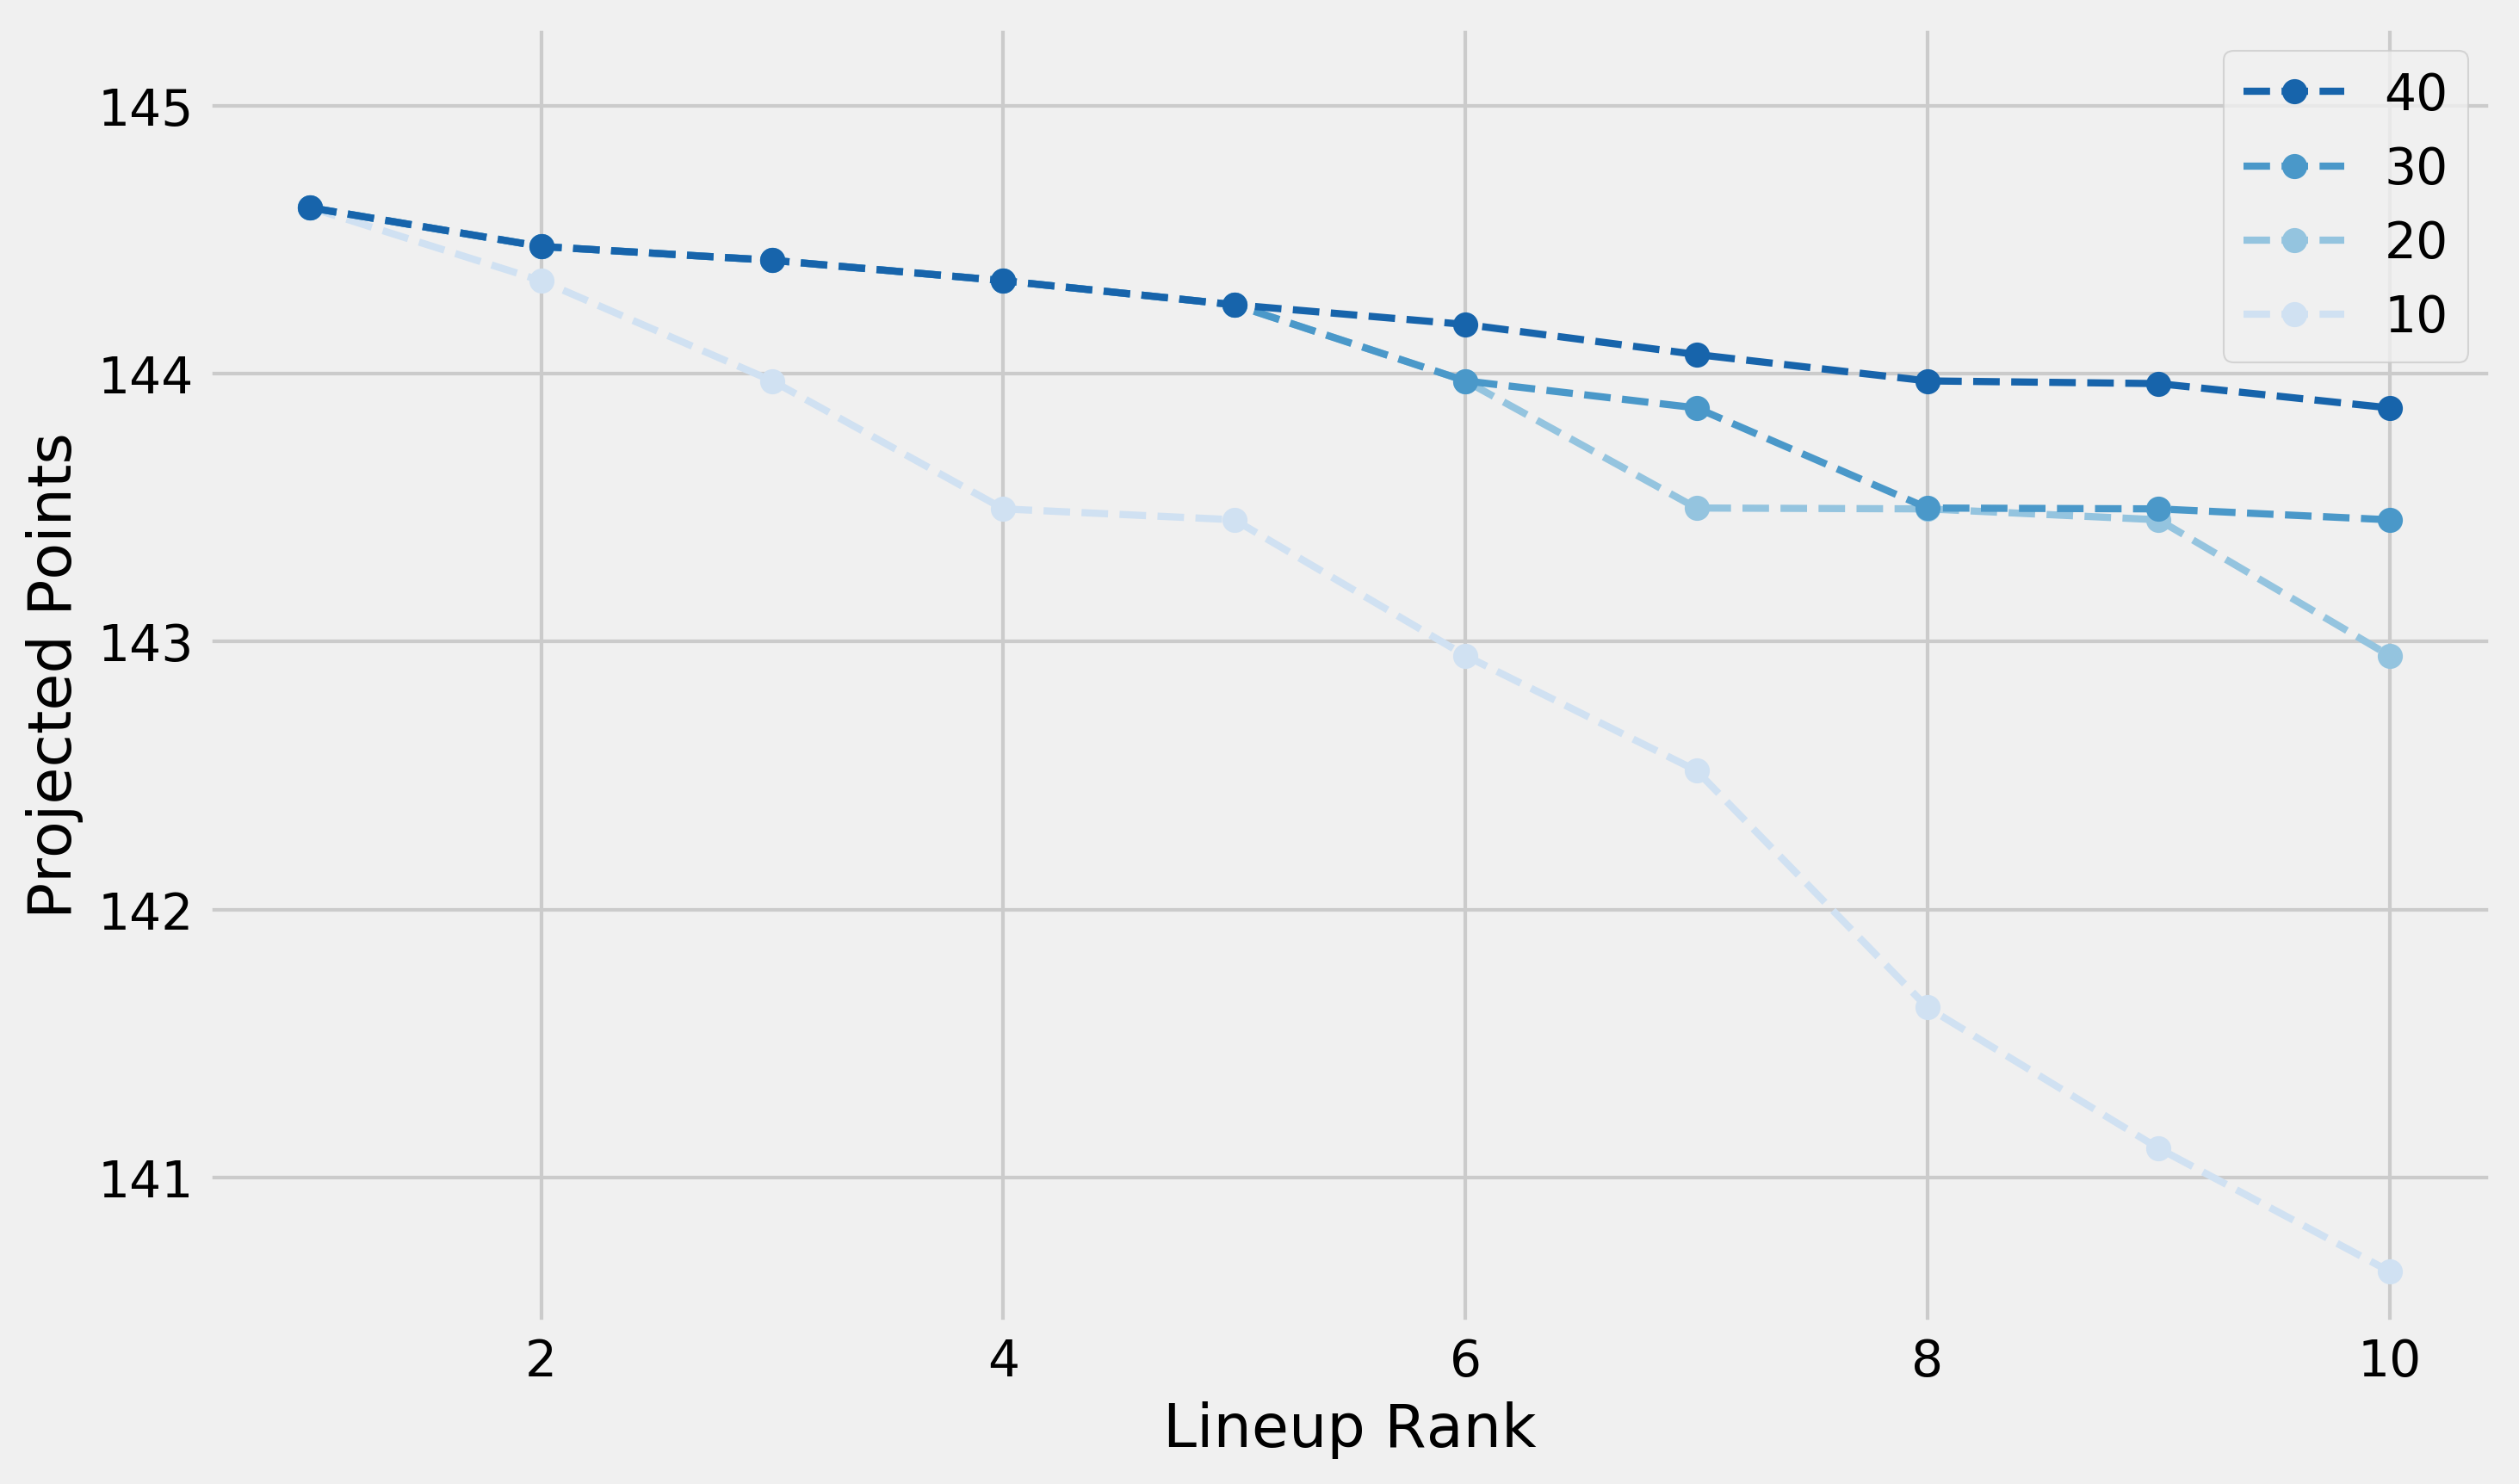
\includegraphics[width=1\textwidth]{../figures/lineups10_vs_n}
    \caption{Top 10 lineups.}
  \end{subfigure}
  \par\bigskip
  \begin{subfigure}[b]{0.80\textwidth}
    \centering
    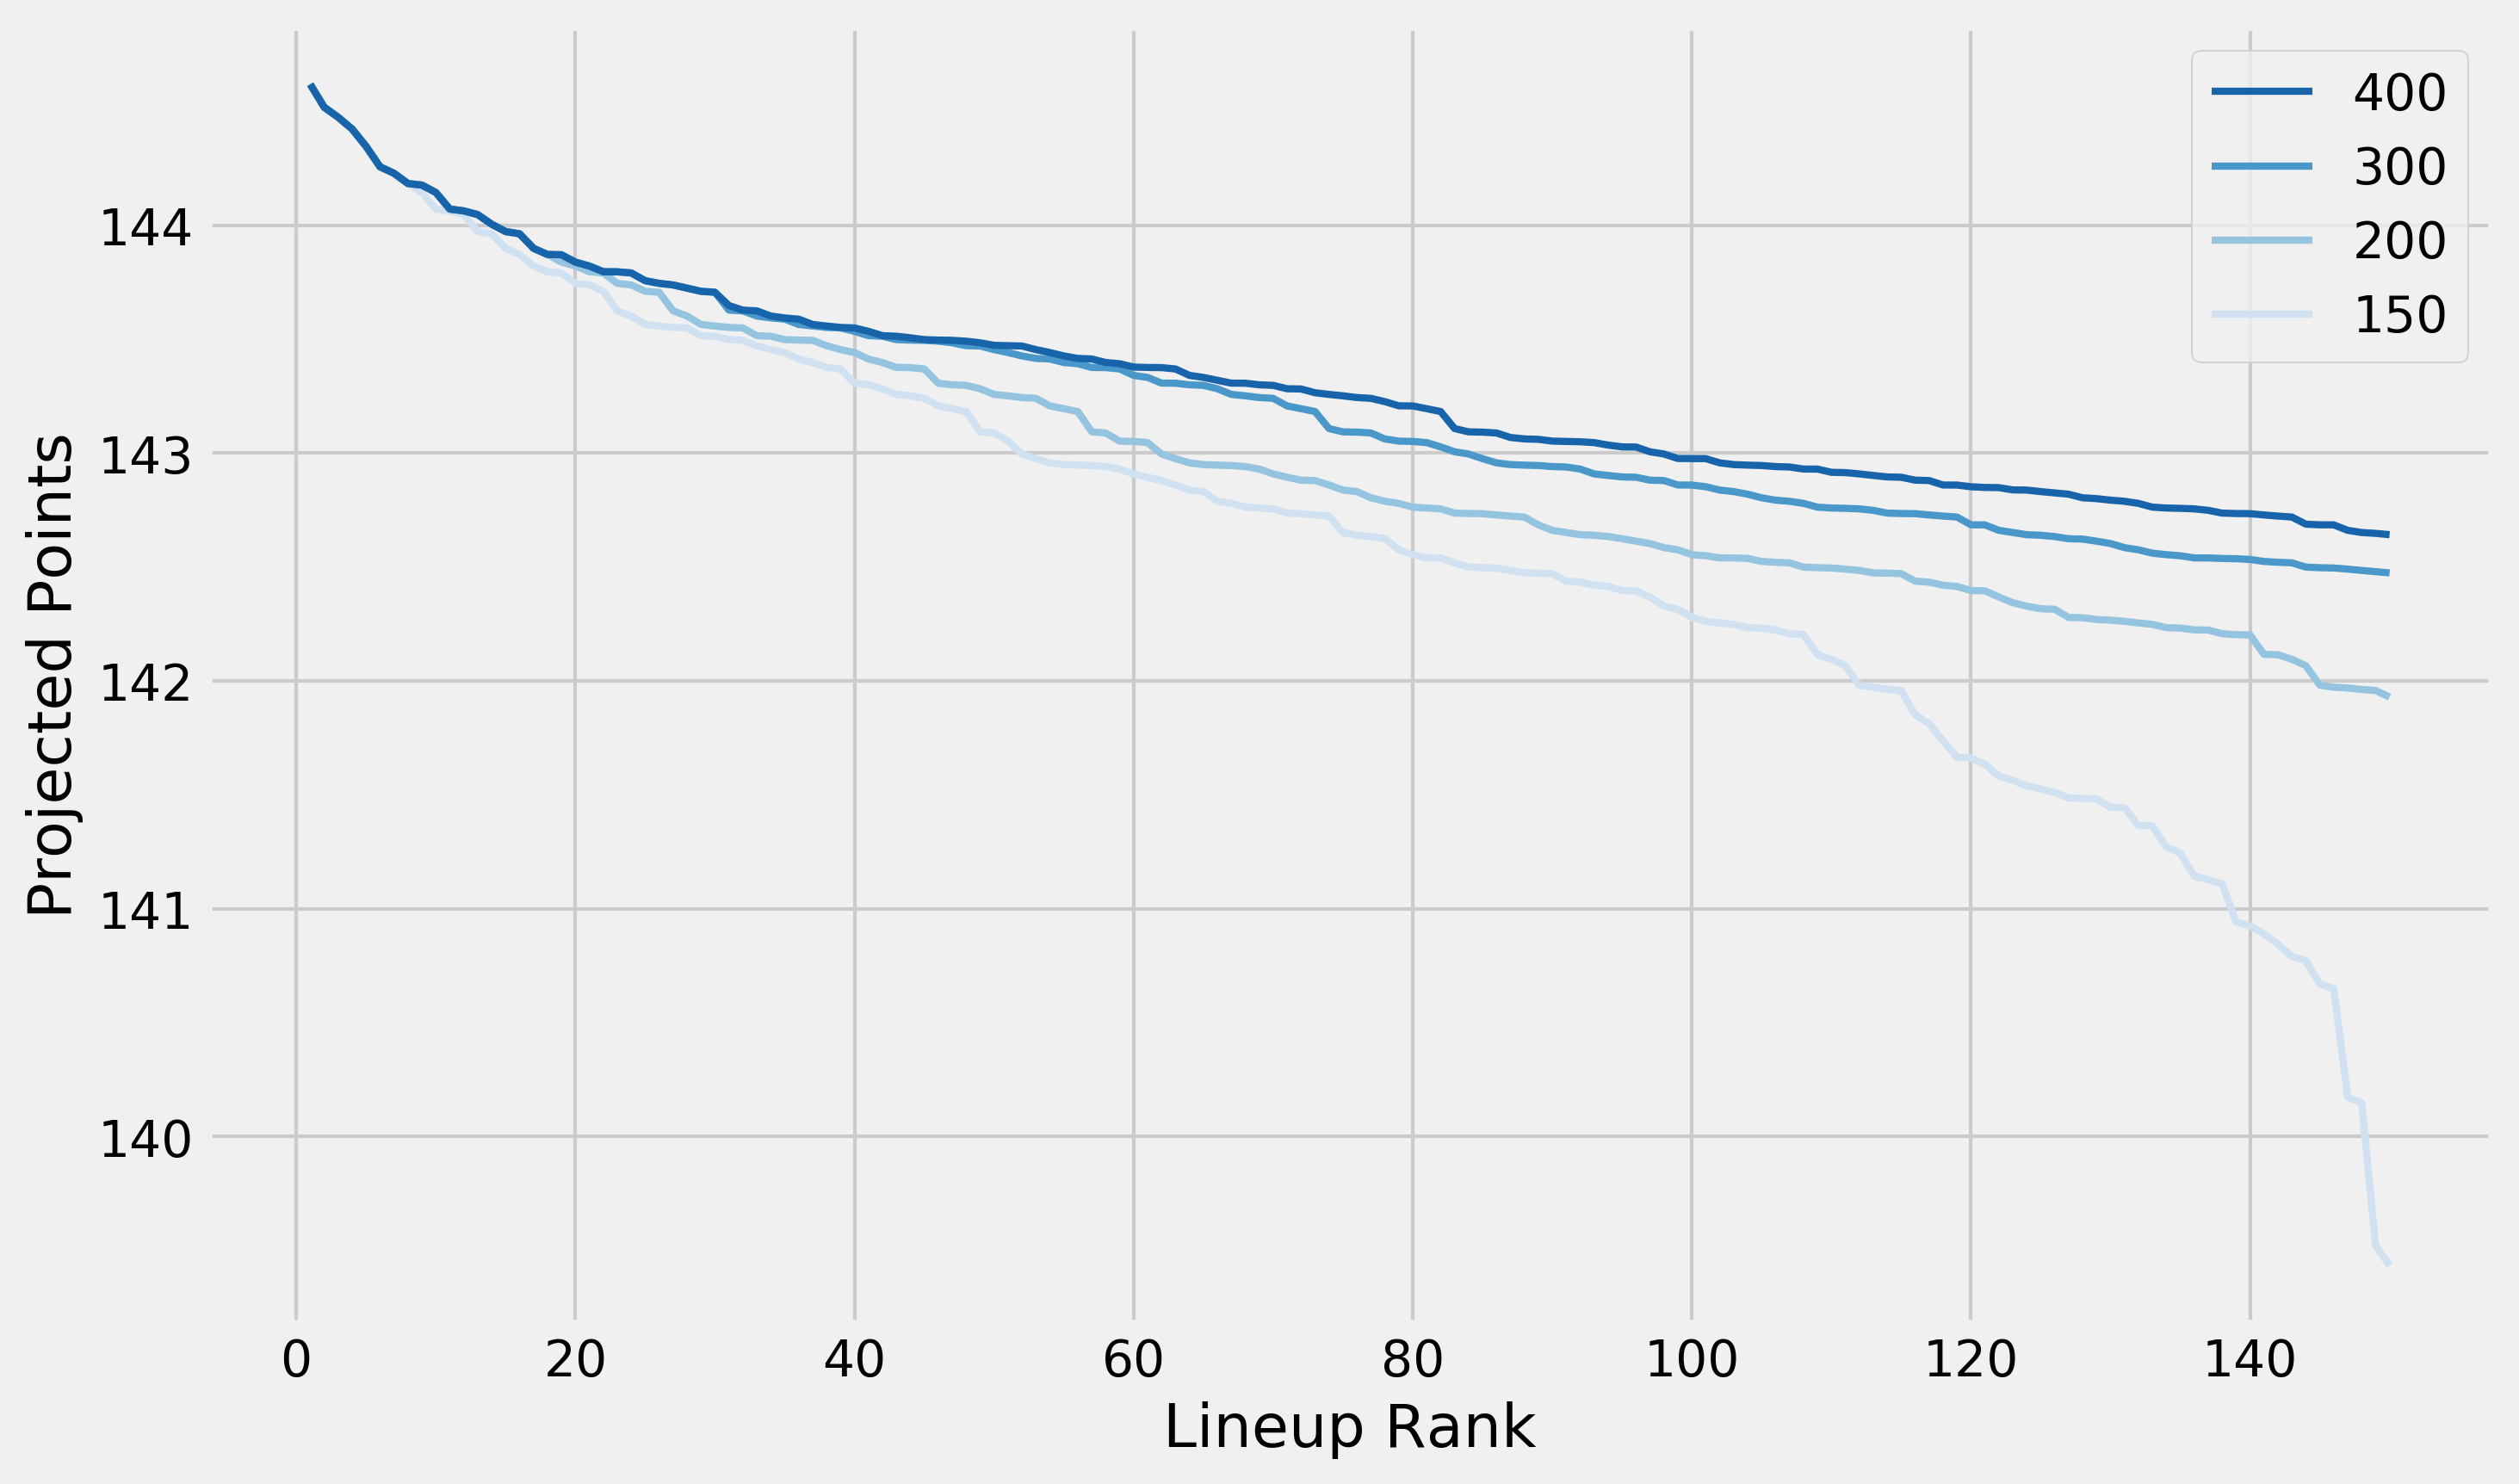
\includegraphics[width=1\textwidth]{../figures/lineups150_vs_n}
    \caption{Top 150 lineups.}
  \end{subfigure}
  \caption{Projected points are plotted against lineup rank for the first $n$ lineups generated.}
\label{lineups_vs_n}
\end{figure}

From Figure \ref{lineups_vs_n}, it is clear that if $n$ lineups are needed, naively choosing $n$ lineups to generate will produce a sub-optimal output.

\pagebreak
\section{Results}
TODO: 



\pagebreak
\section{Conclusion}
TODO: conclusions

% ------------------------------------ References ---------------------------------------------- %

\pagebreak
\begin{thebibliography}{}

\bibitem{fancyimpute}
A. Rubinsteyn, \& S. Feldman (2019). 
``A Variety of Matrix Completion and Imputation Algorithms Implemented in Python.'' \url{https://github.com/iskandr/fancyimpute}





\end{thebibliography}

\pagebreak
\section{Appendix}
\subsection{Nonessential Stats Summary}

\begin{figure}[H]
  \centering
  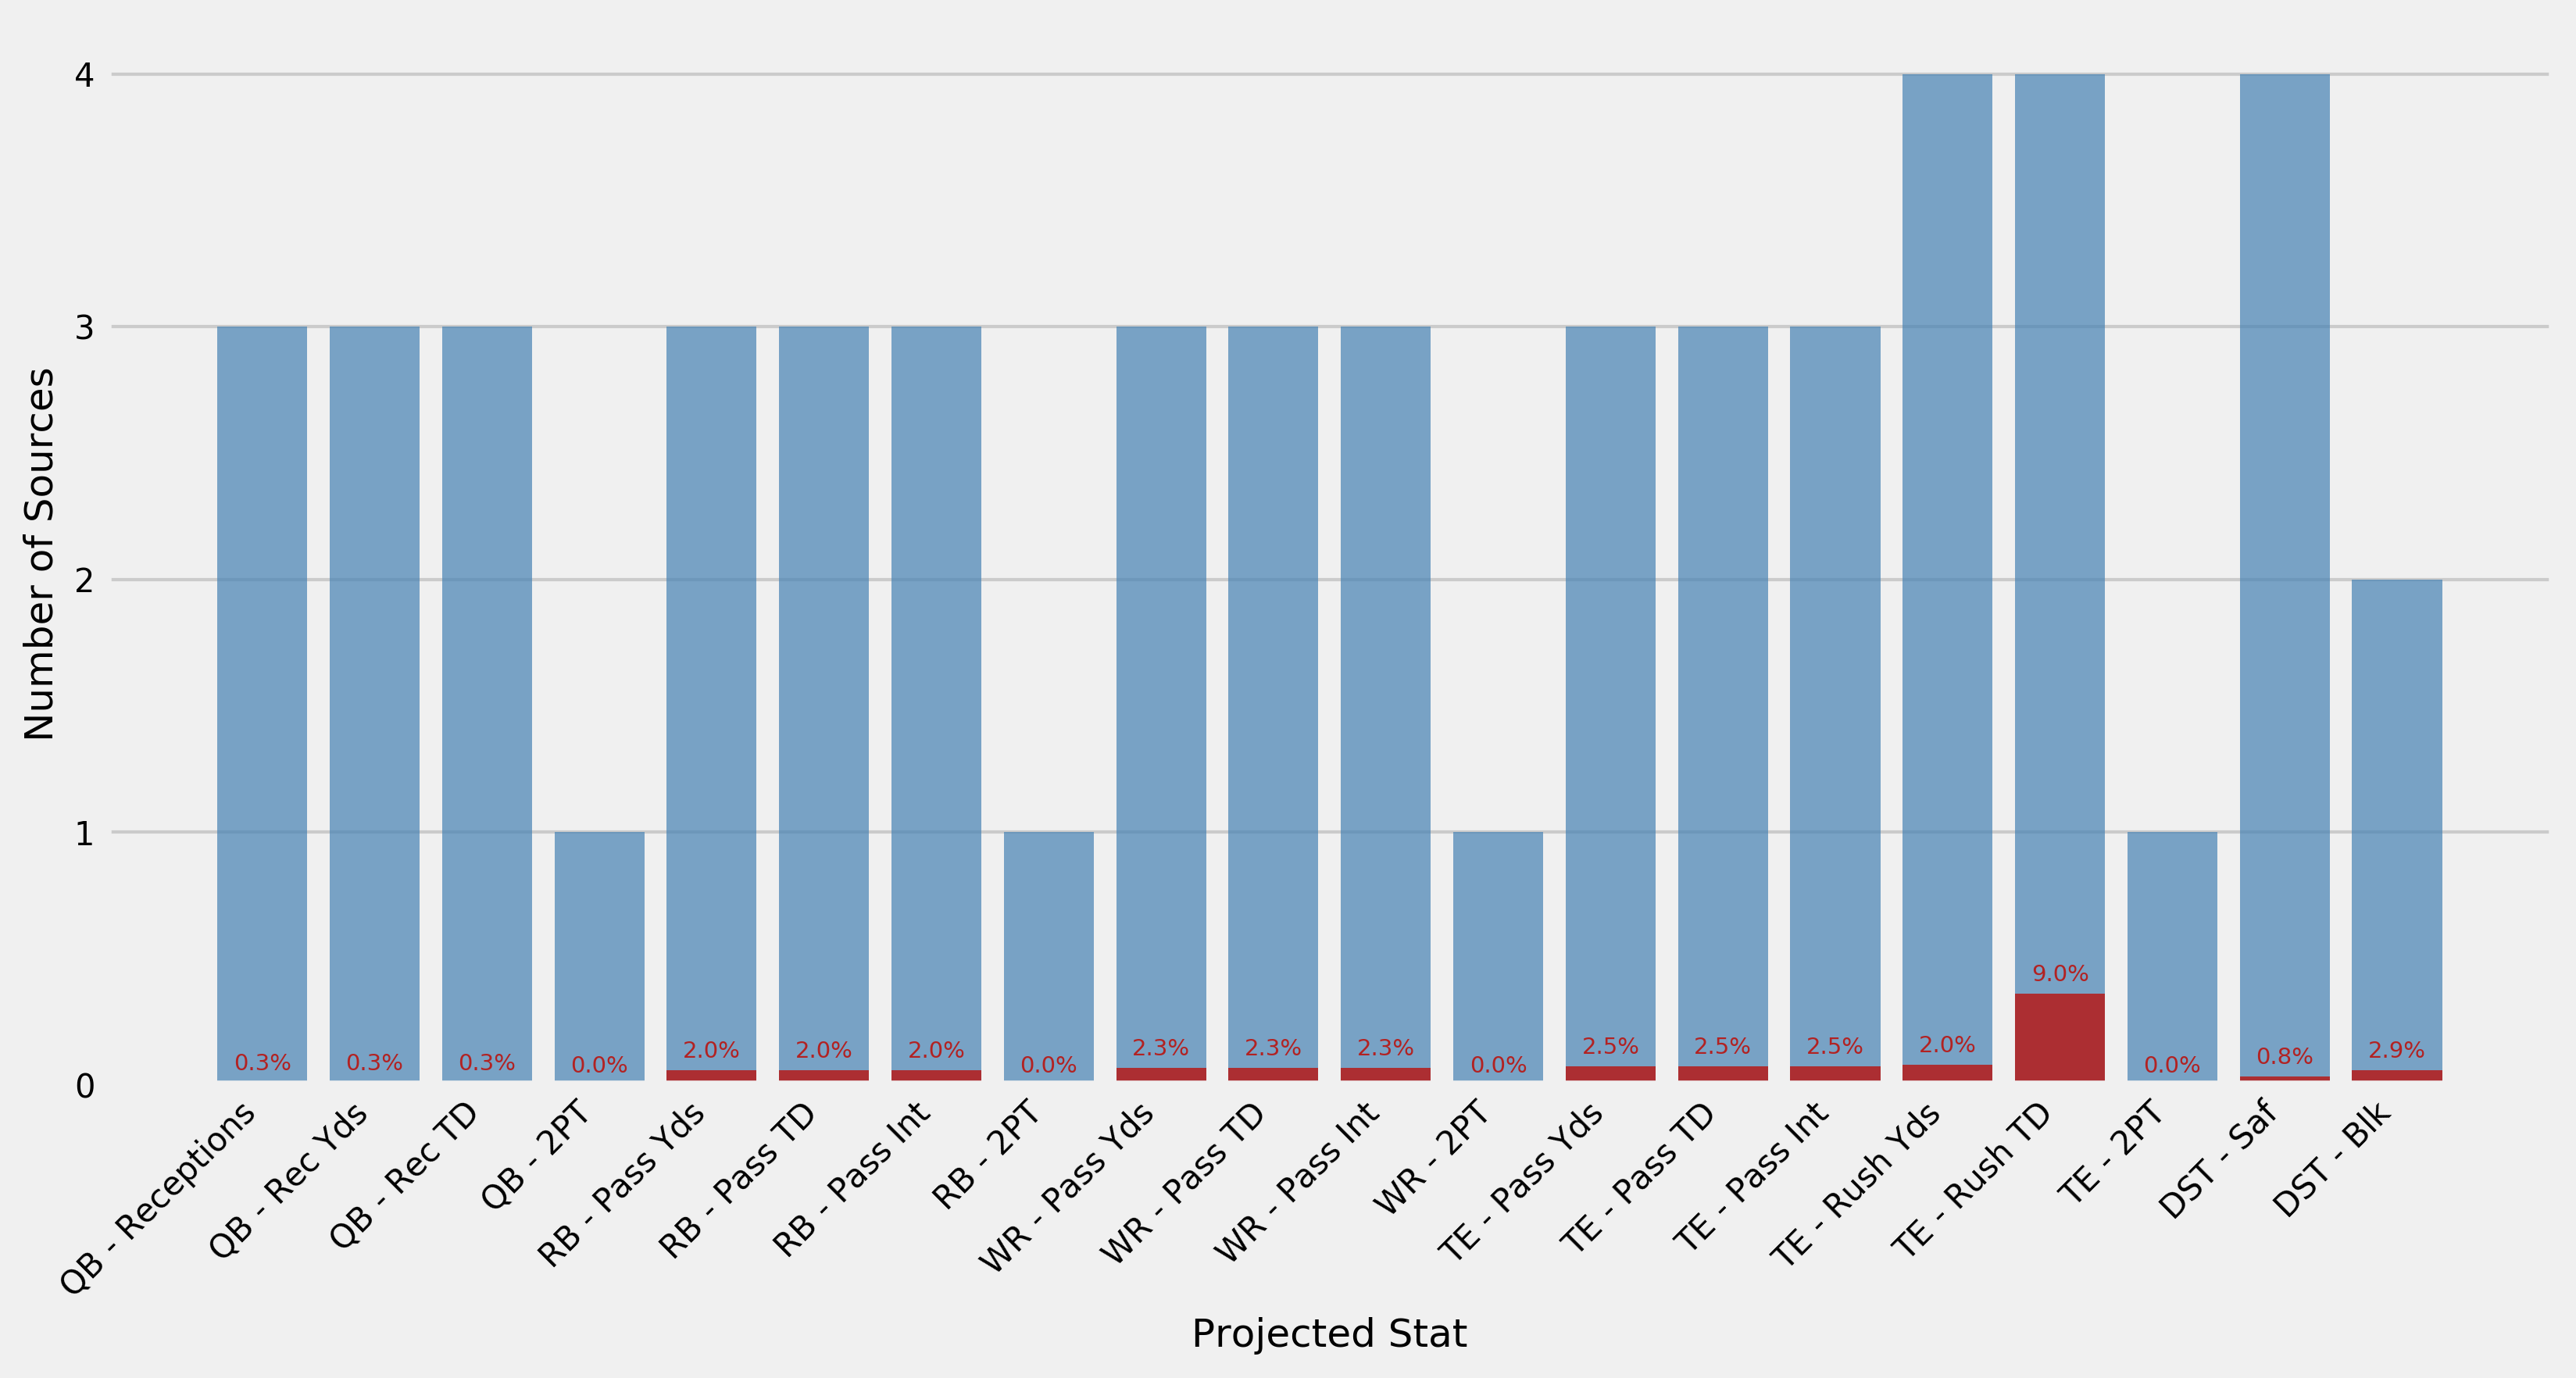
\includegraphics[width=0.95\textwidth]{../figures/nonessential_missing_data}
  \caption{Number of sources collected for each nonessential stat (blue). Red  indicates percentage of missing data for each respective stat.}
\end{figure}

\begin{figure}[H]
  \centering
  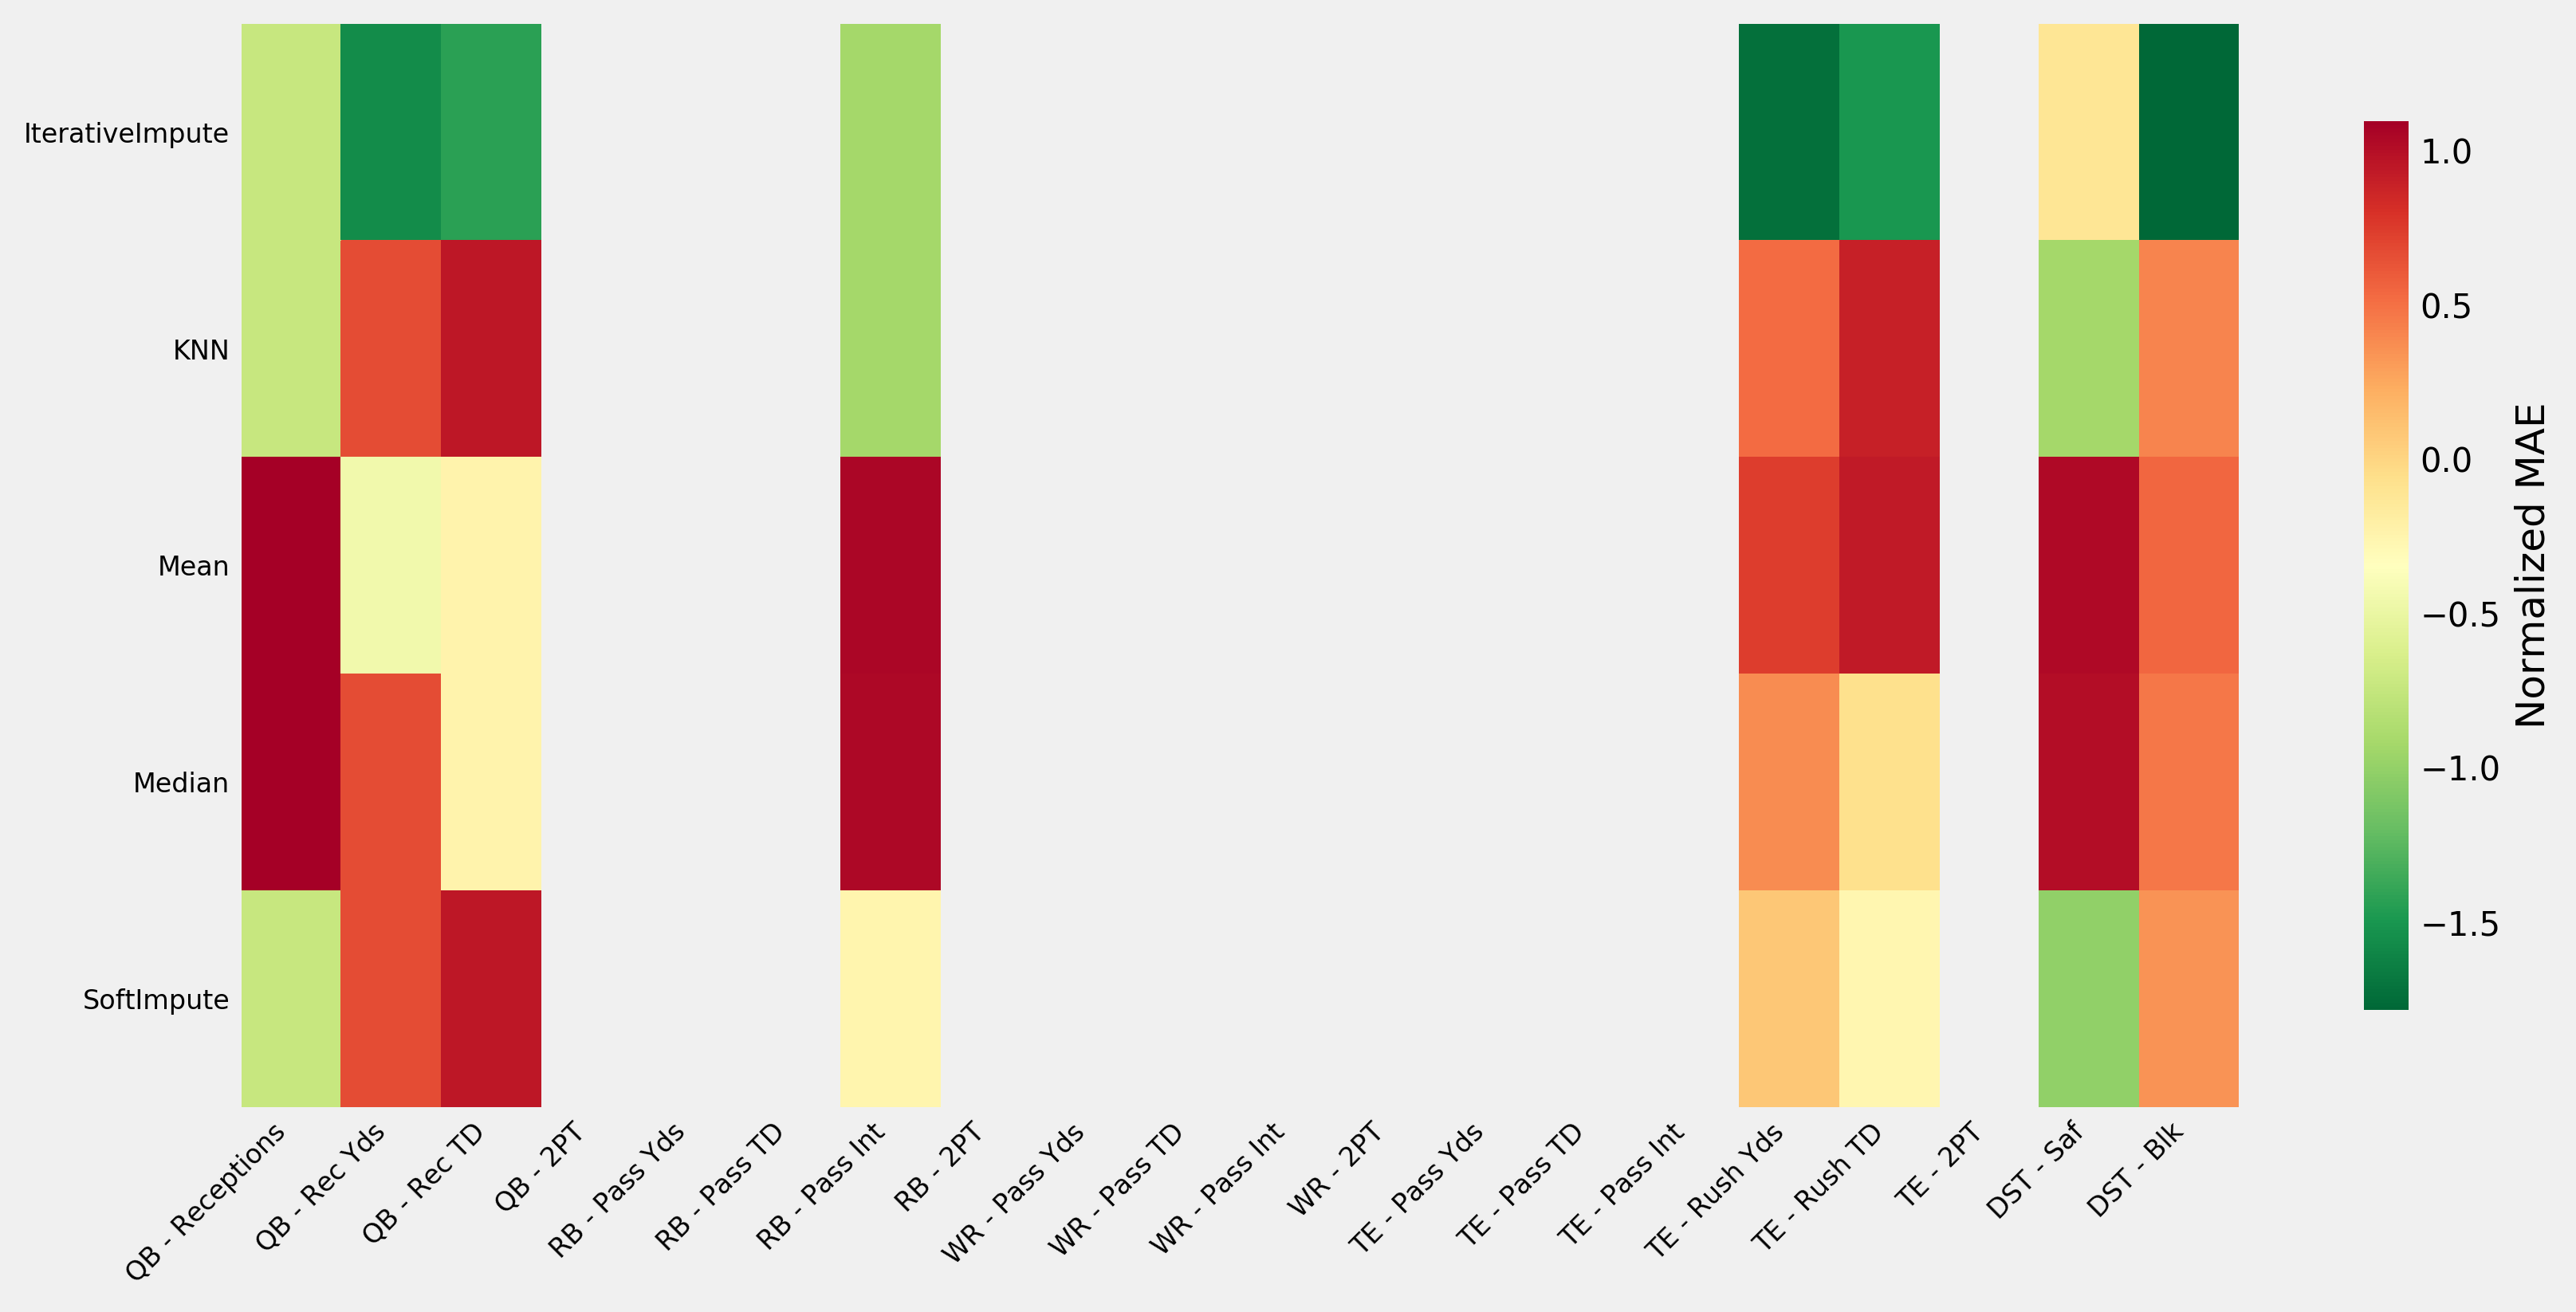
\includegraphics[width=0.95\textwidth]{../figures/nonessential_impute_MAE}
  \caption{Normalized MAE of imputing methods for each nonessential stat.}
\end{figure}

\begin{figure}[H]
  \centering
  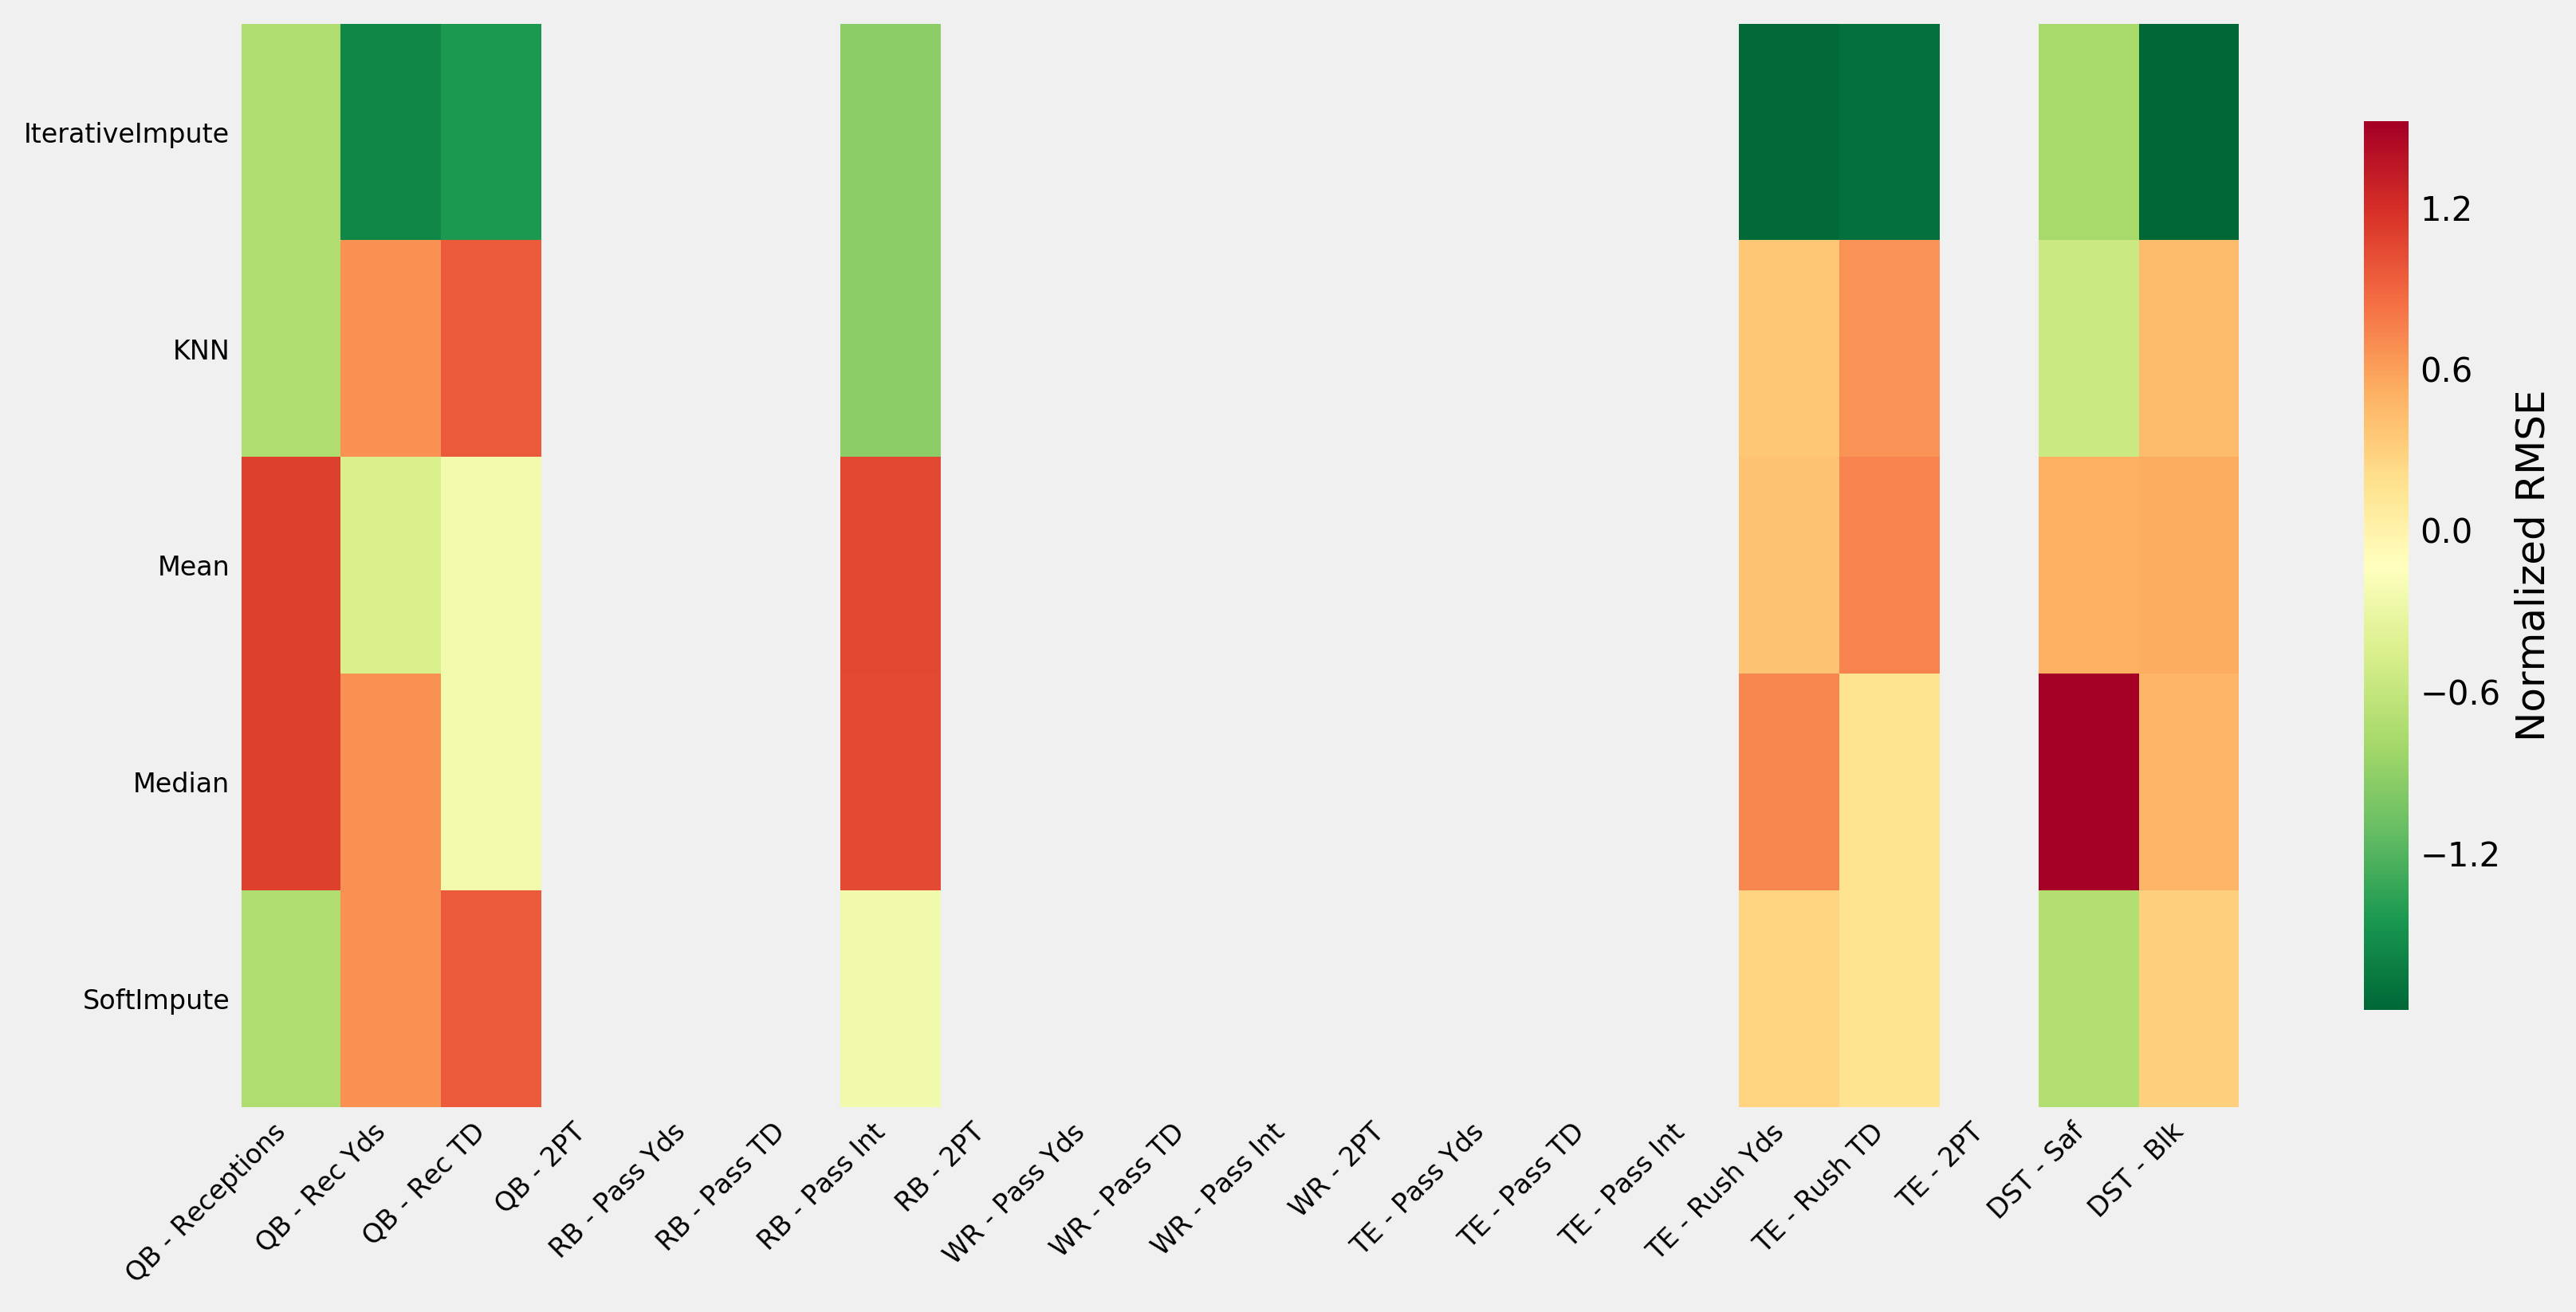
\includegraphics[width=0.95\textwidth]{../figures/nonessential_impute_RMSE}
  \caption{Normalized RMSE of imputing methods for each nonessential stat.}
\end{figure}

\pagebreak
\section{Essential Stats Histograms}

\begin{figure}[H]
  \centering
  \begin{subfigure}[b]{0.450\textwidth}
    \centering
    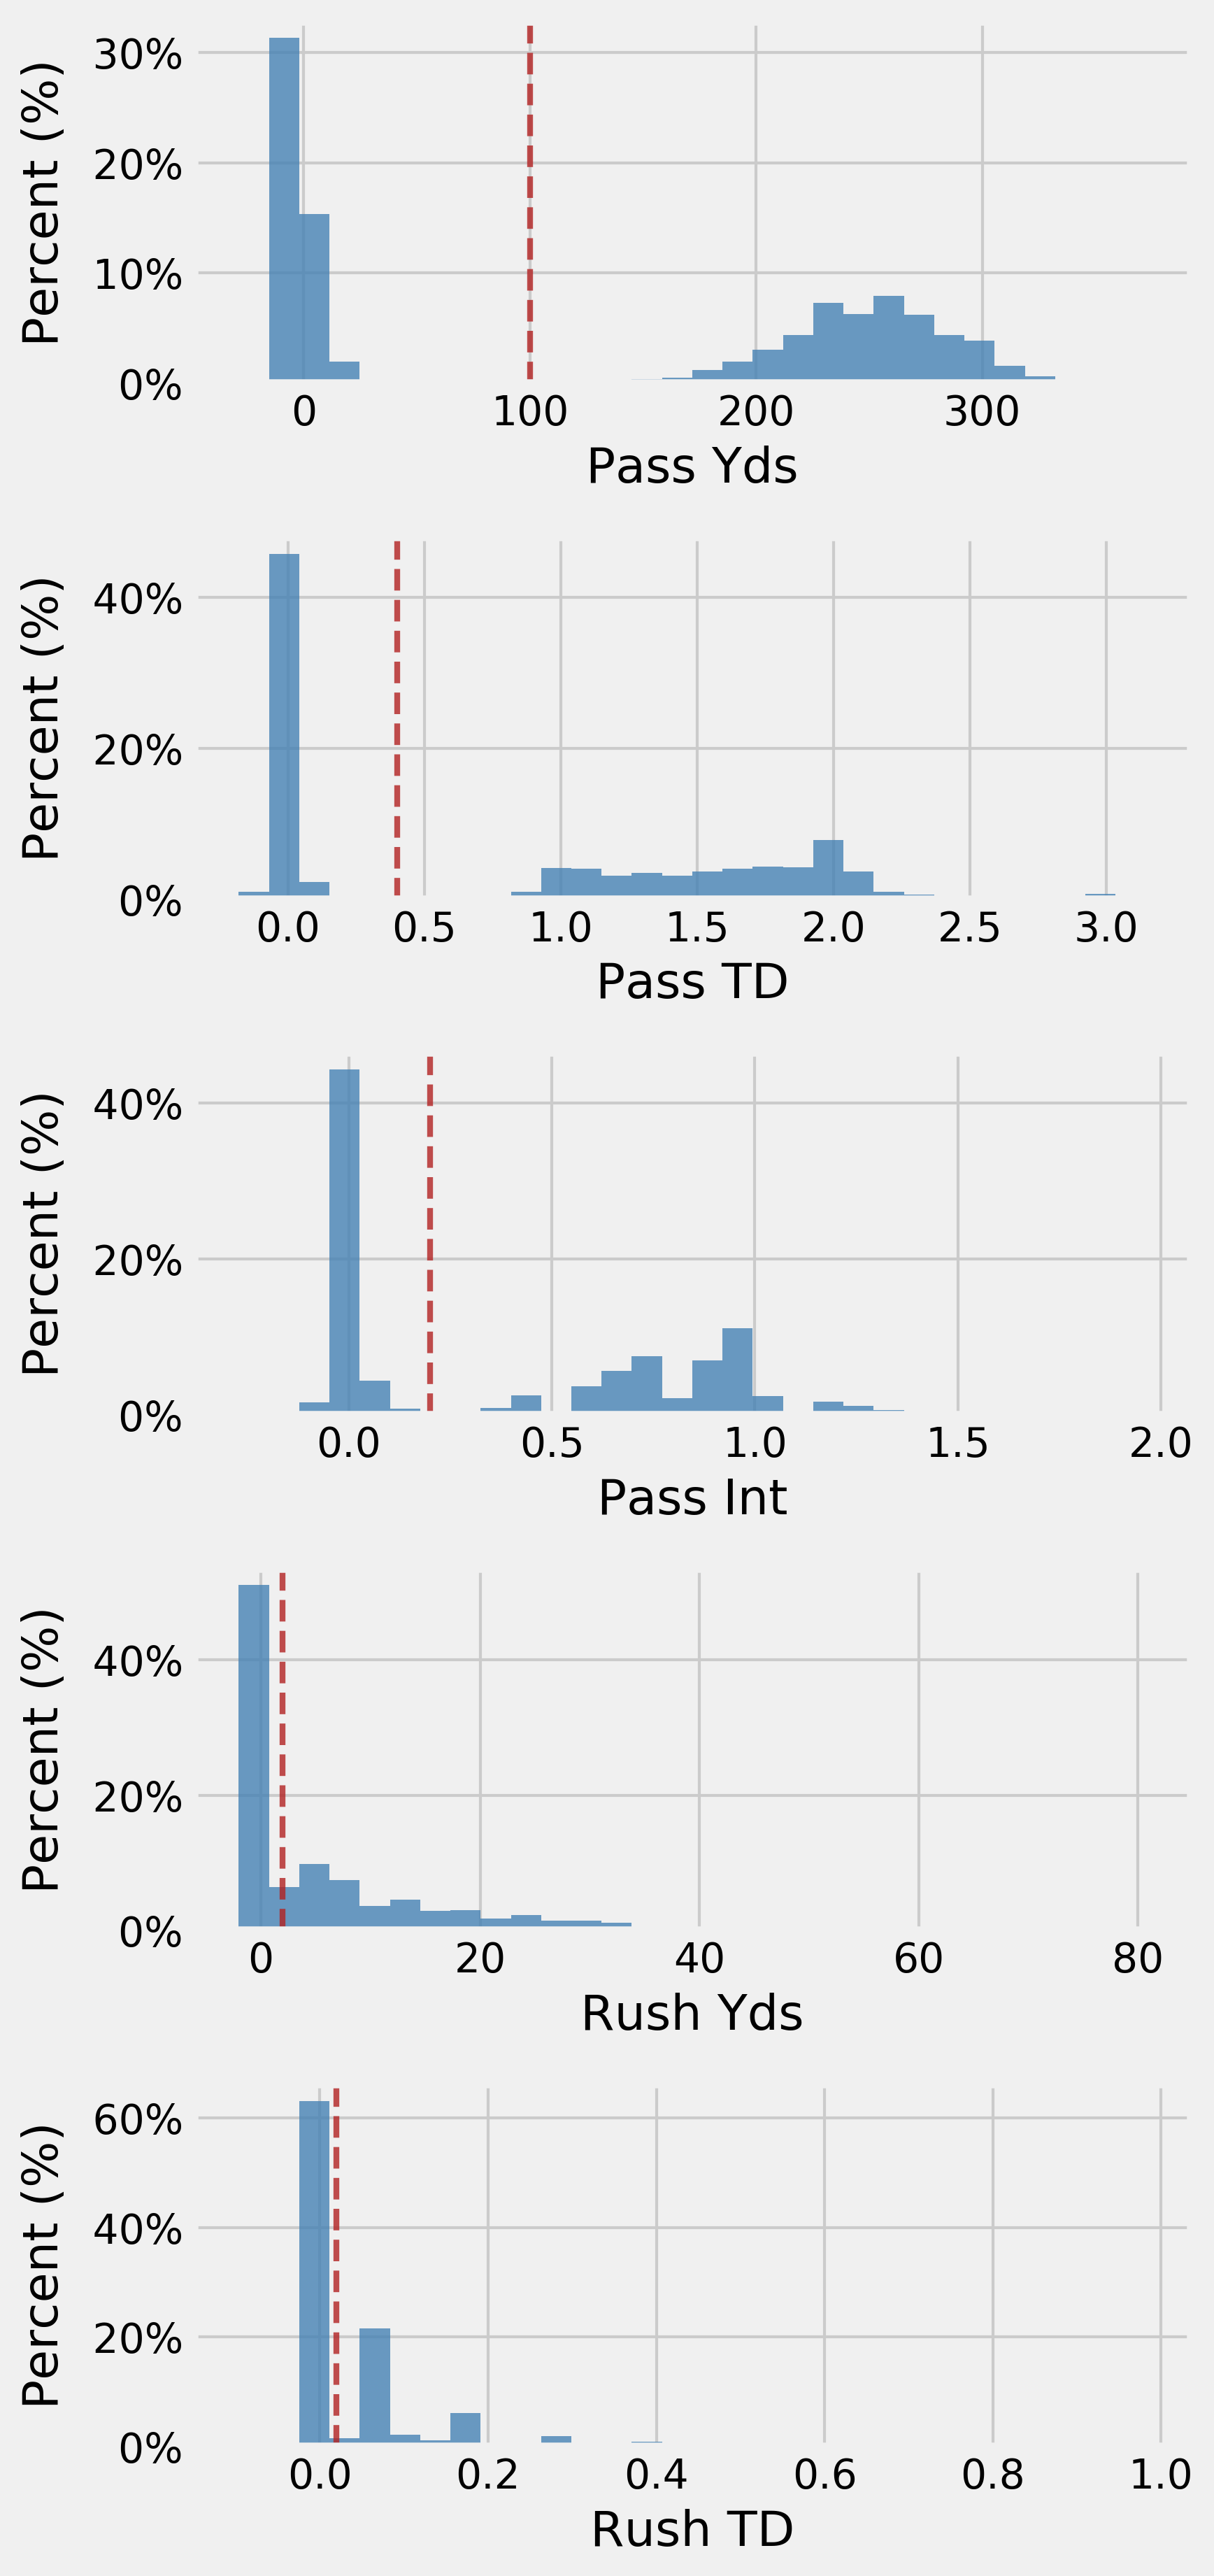
\includegraphics[width=1\textwidth]{../figures/no_threshold_hist_QB}
    \caption{Raw histogram with threshold (red).}
  \end{subfigure}
  \hfill
  \begin{subfigure}[b]{0.450\textwidth}
    \centering
    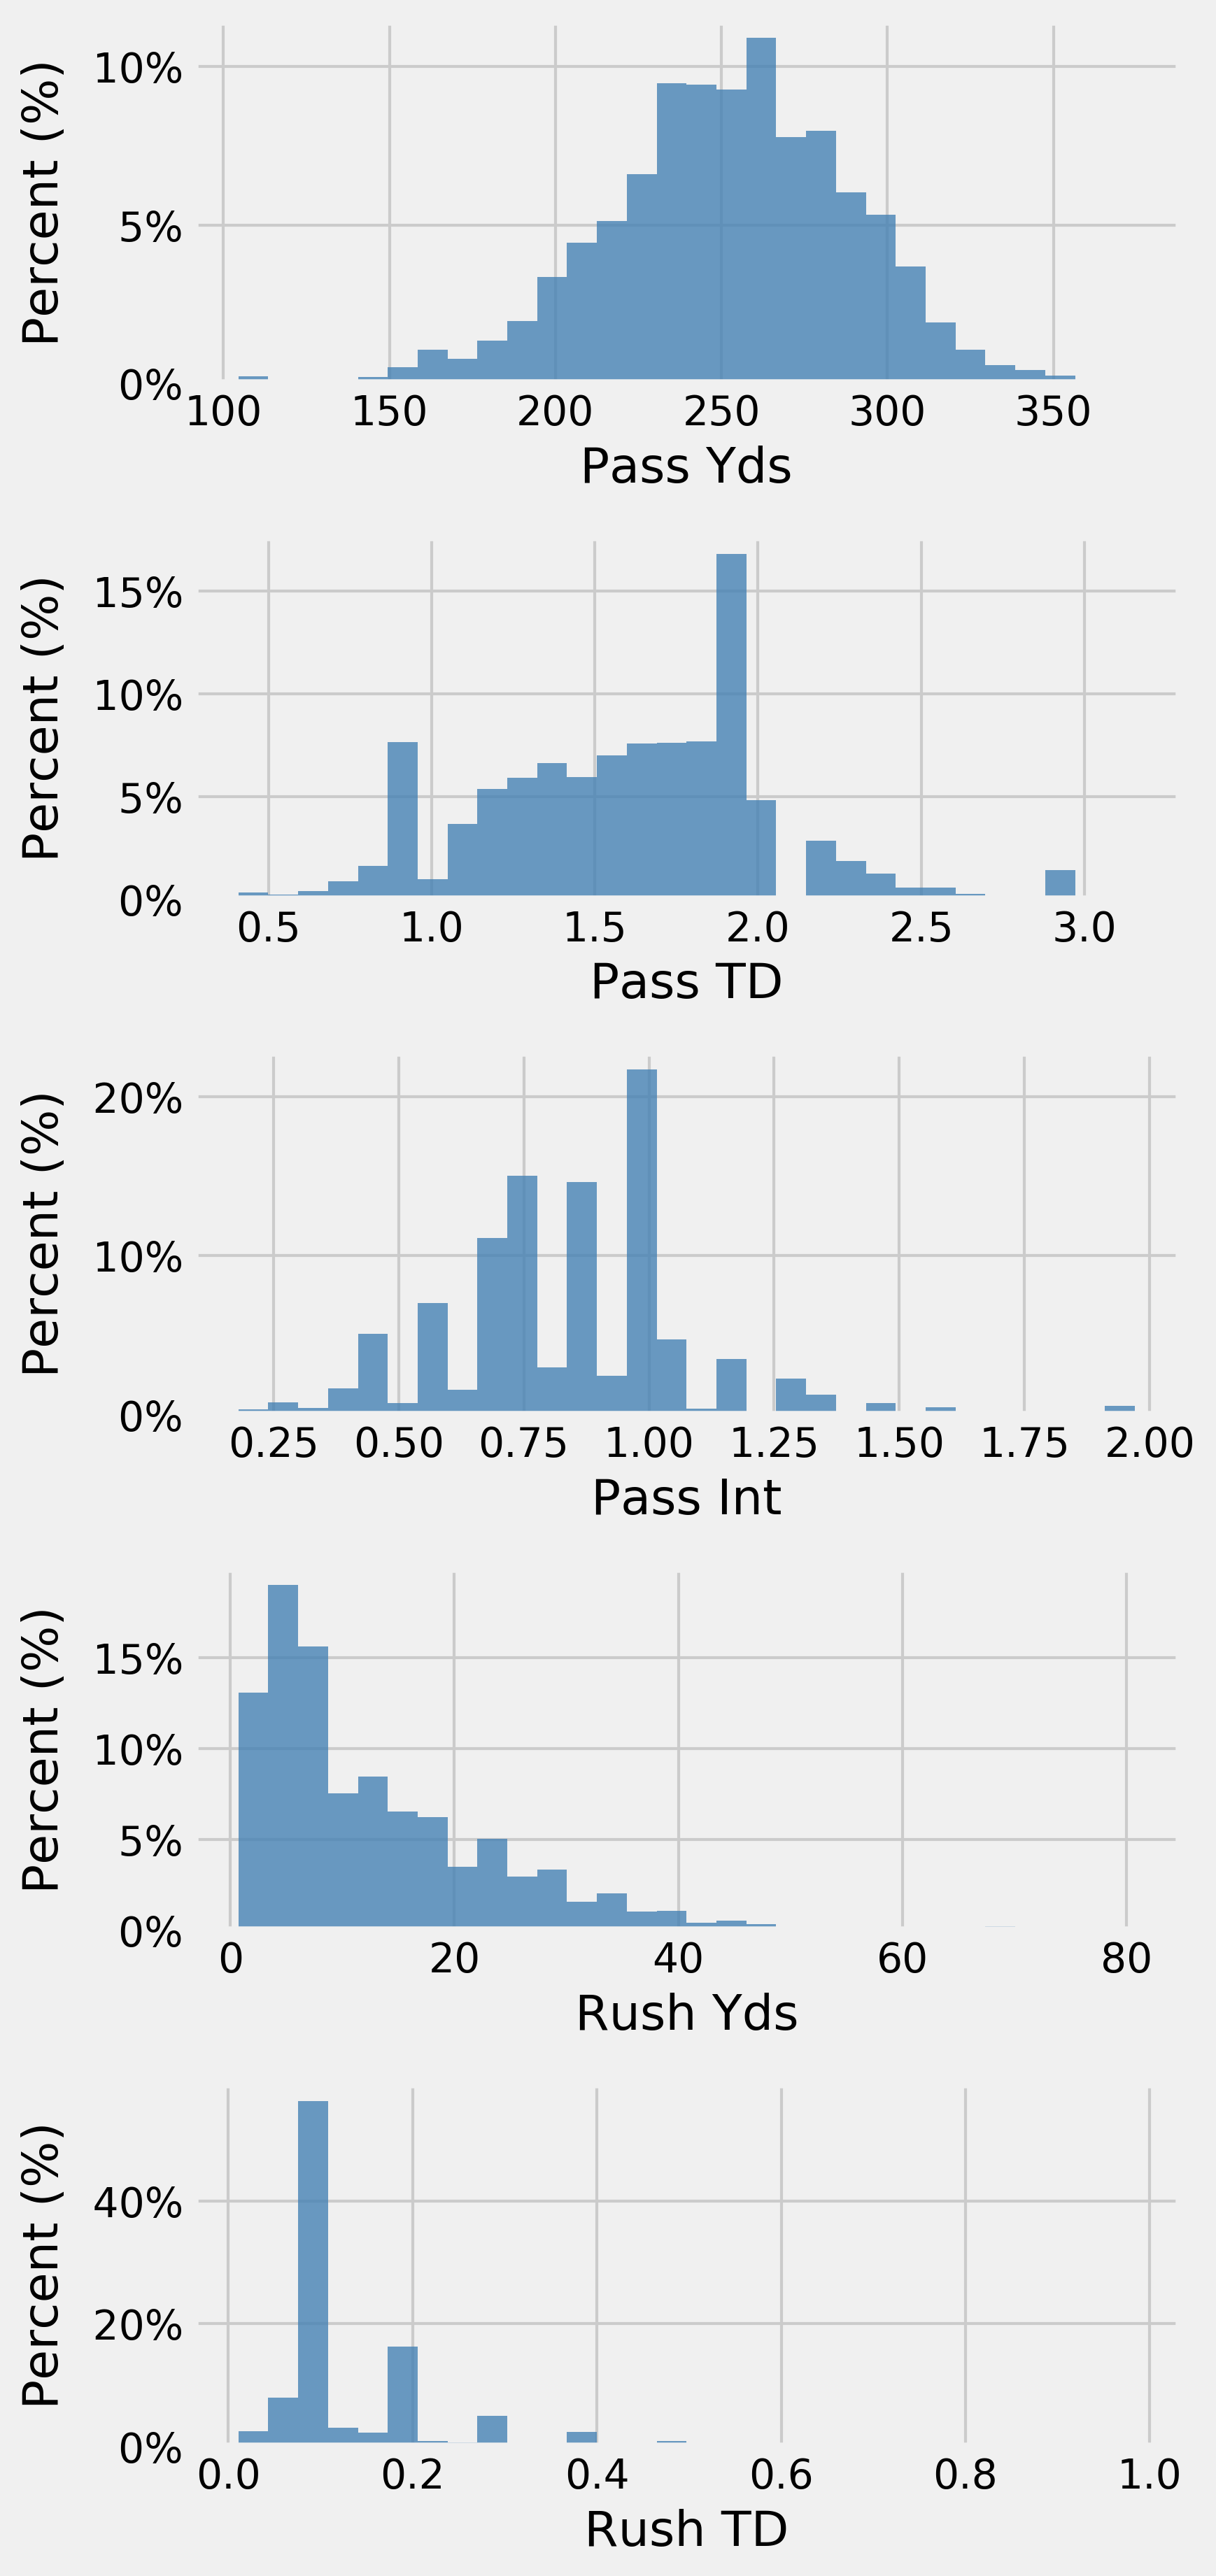
\includegraphics[width=1\textwidth]{../figures/threshold_hist_QB}
    \caption{Histogram above threshold.}
  \end{subfigure}
  \caption{Essential stat raw histograms and thresholded histograms for QB.}
\end{figure}

\pagebreak
\begin{figure}[H]
  \centering
  \begin{subfigure}[b]{0.450\textwidth}
    \centering
    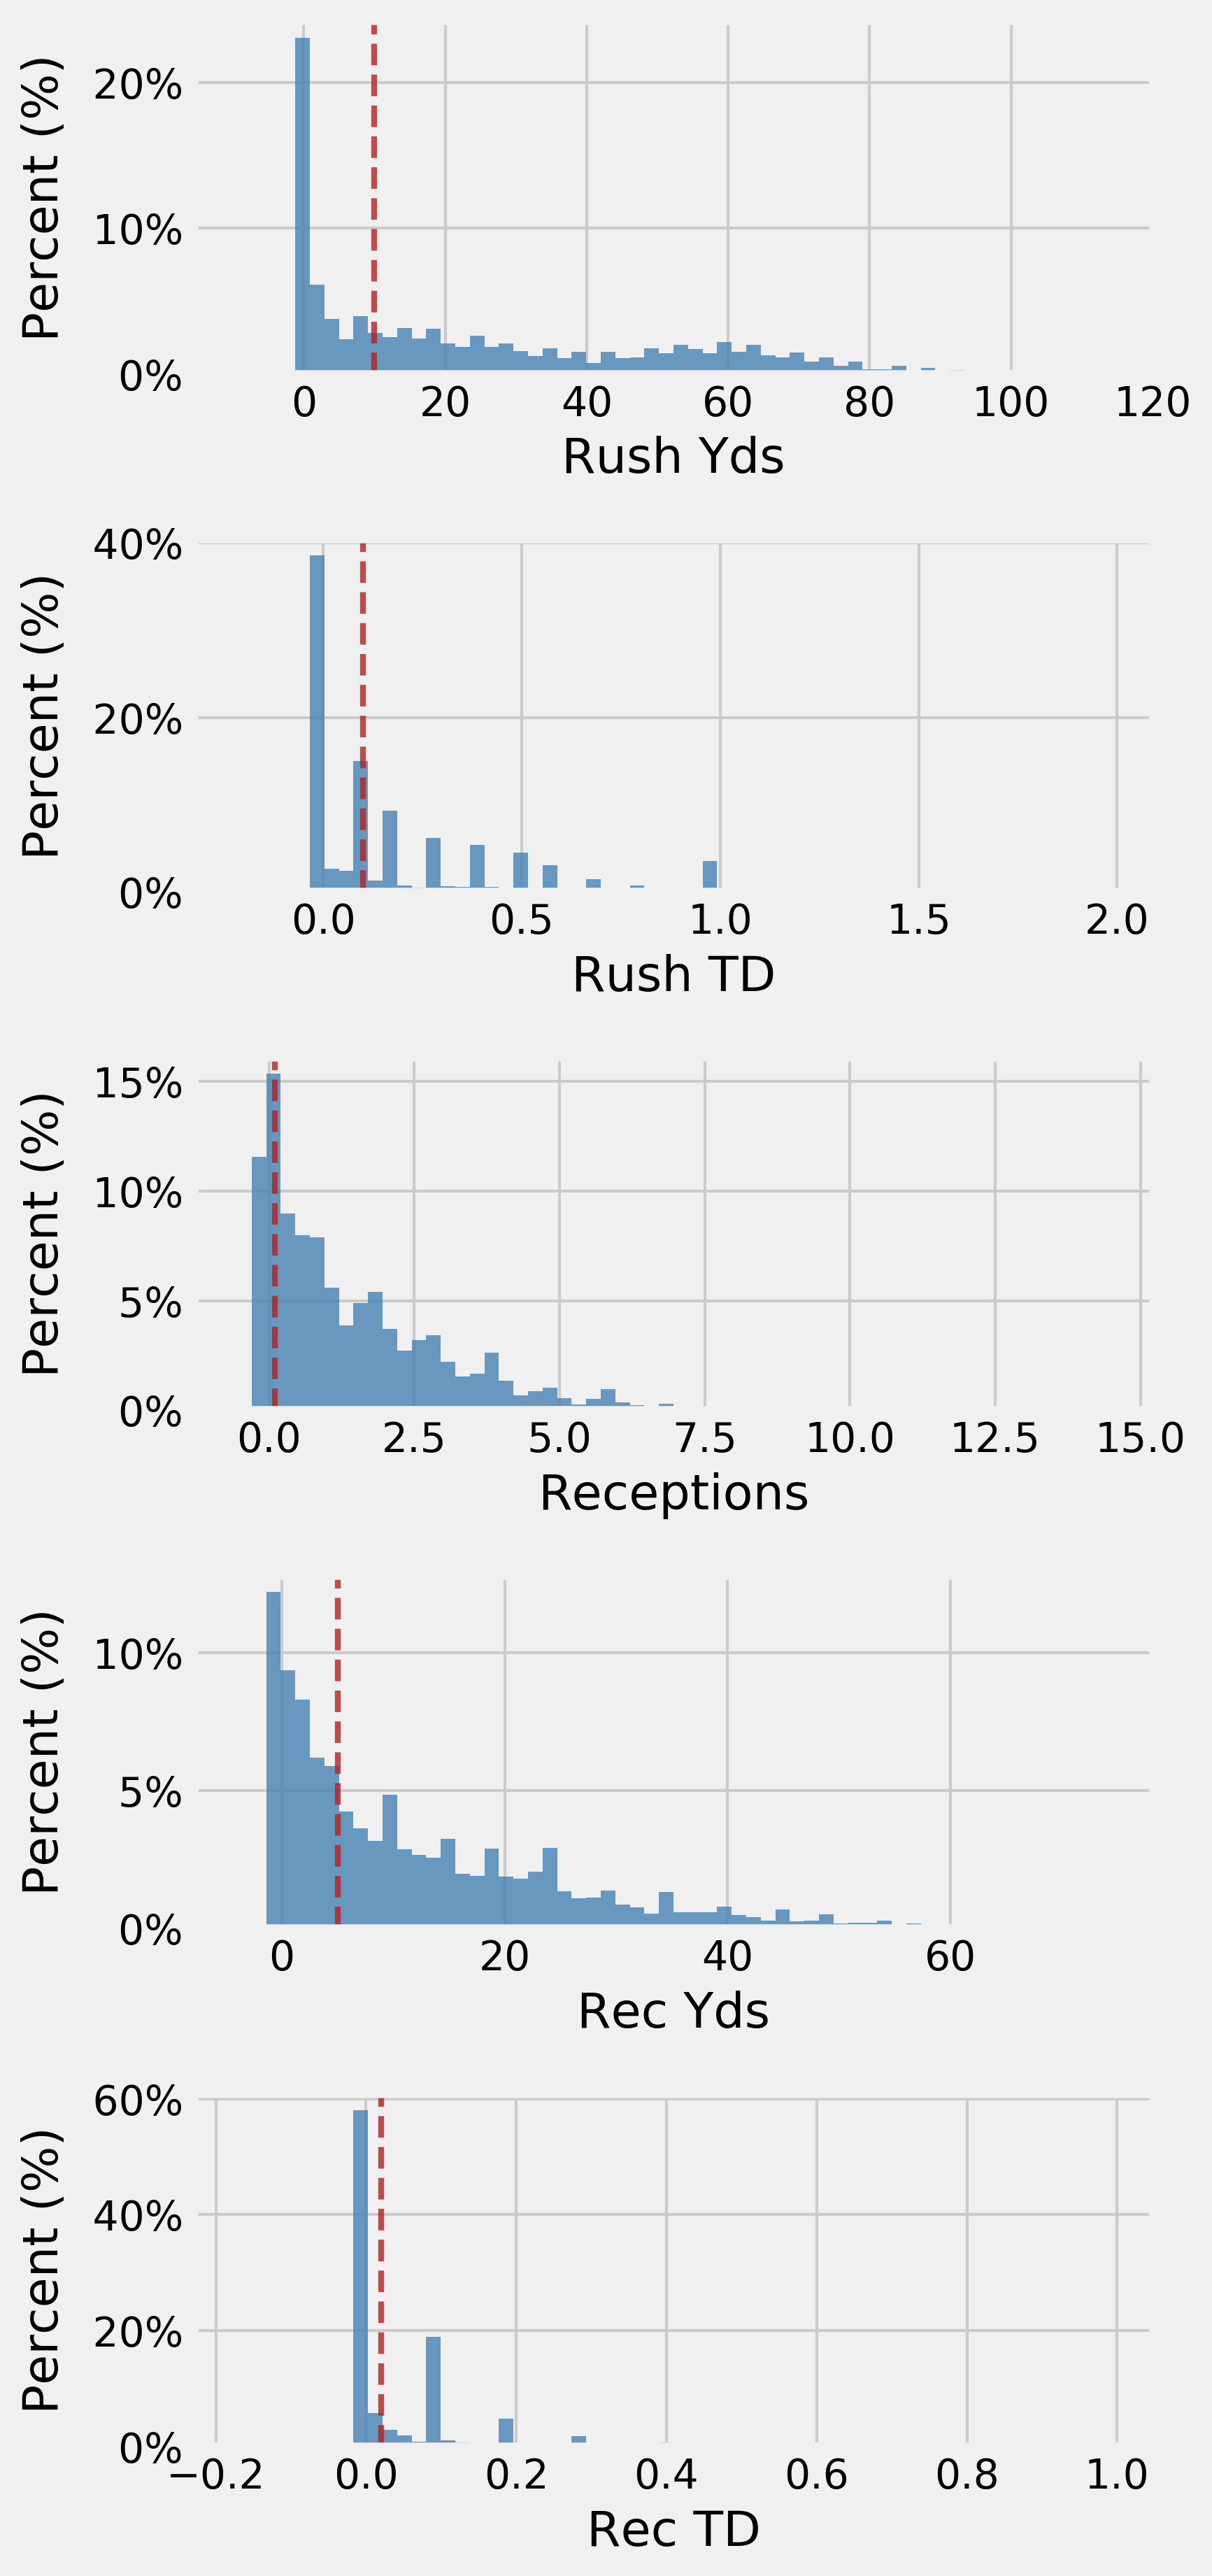
\includegraphics[width=1\textwidth]{../figures/no_threshold_hist_RB}
    \caption{Raw histogram with threshold (red).}
  \end{subfigure}
  \hfill
  \begin{subfigure}[b]{0.450\textwidth}
    \centering
    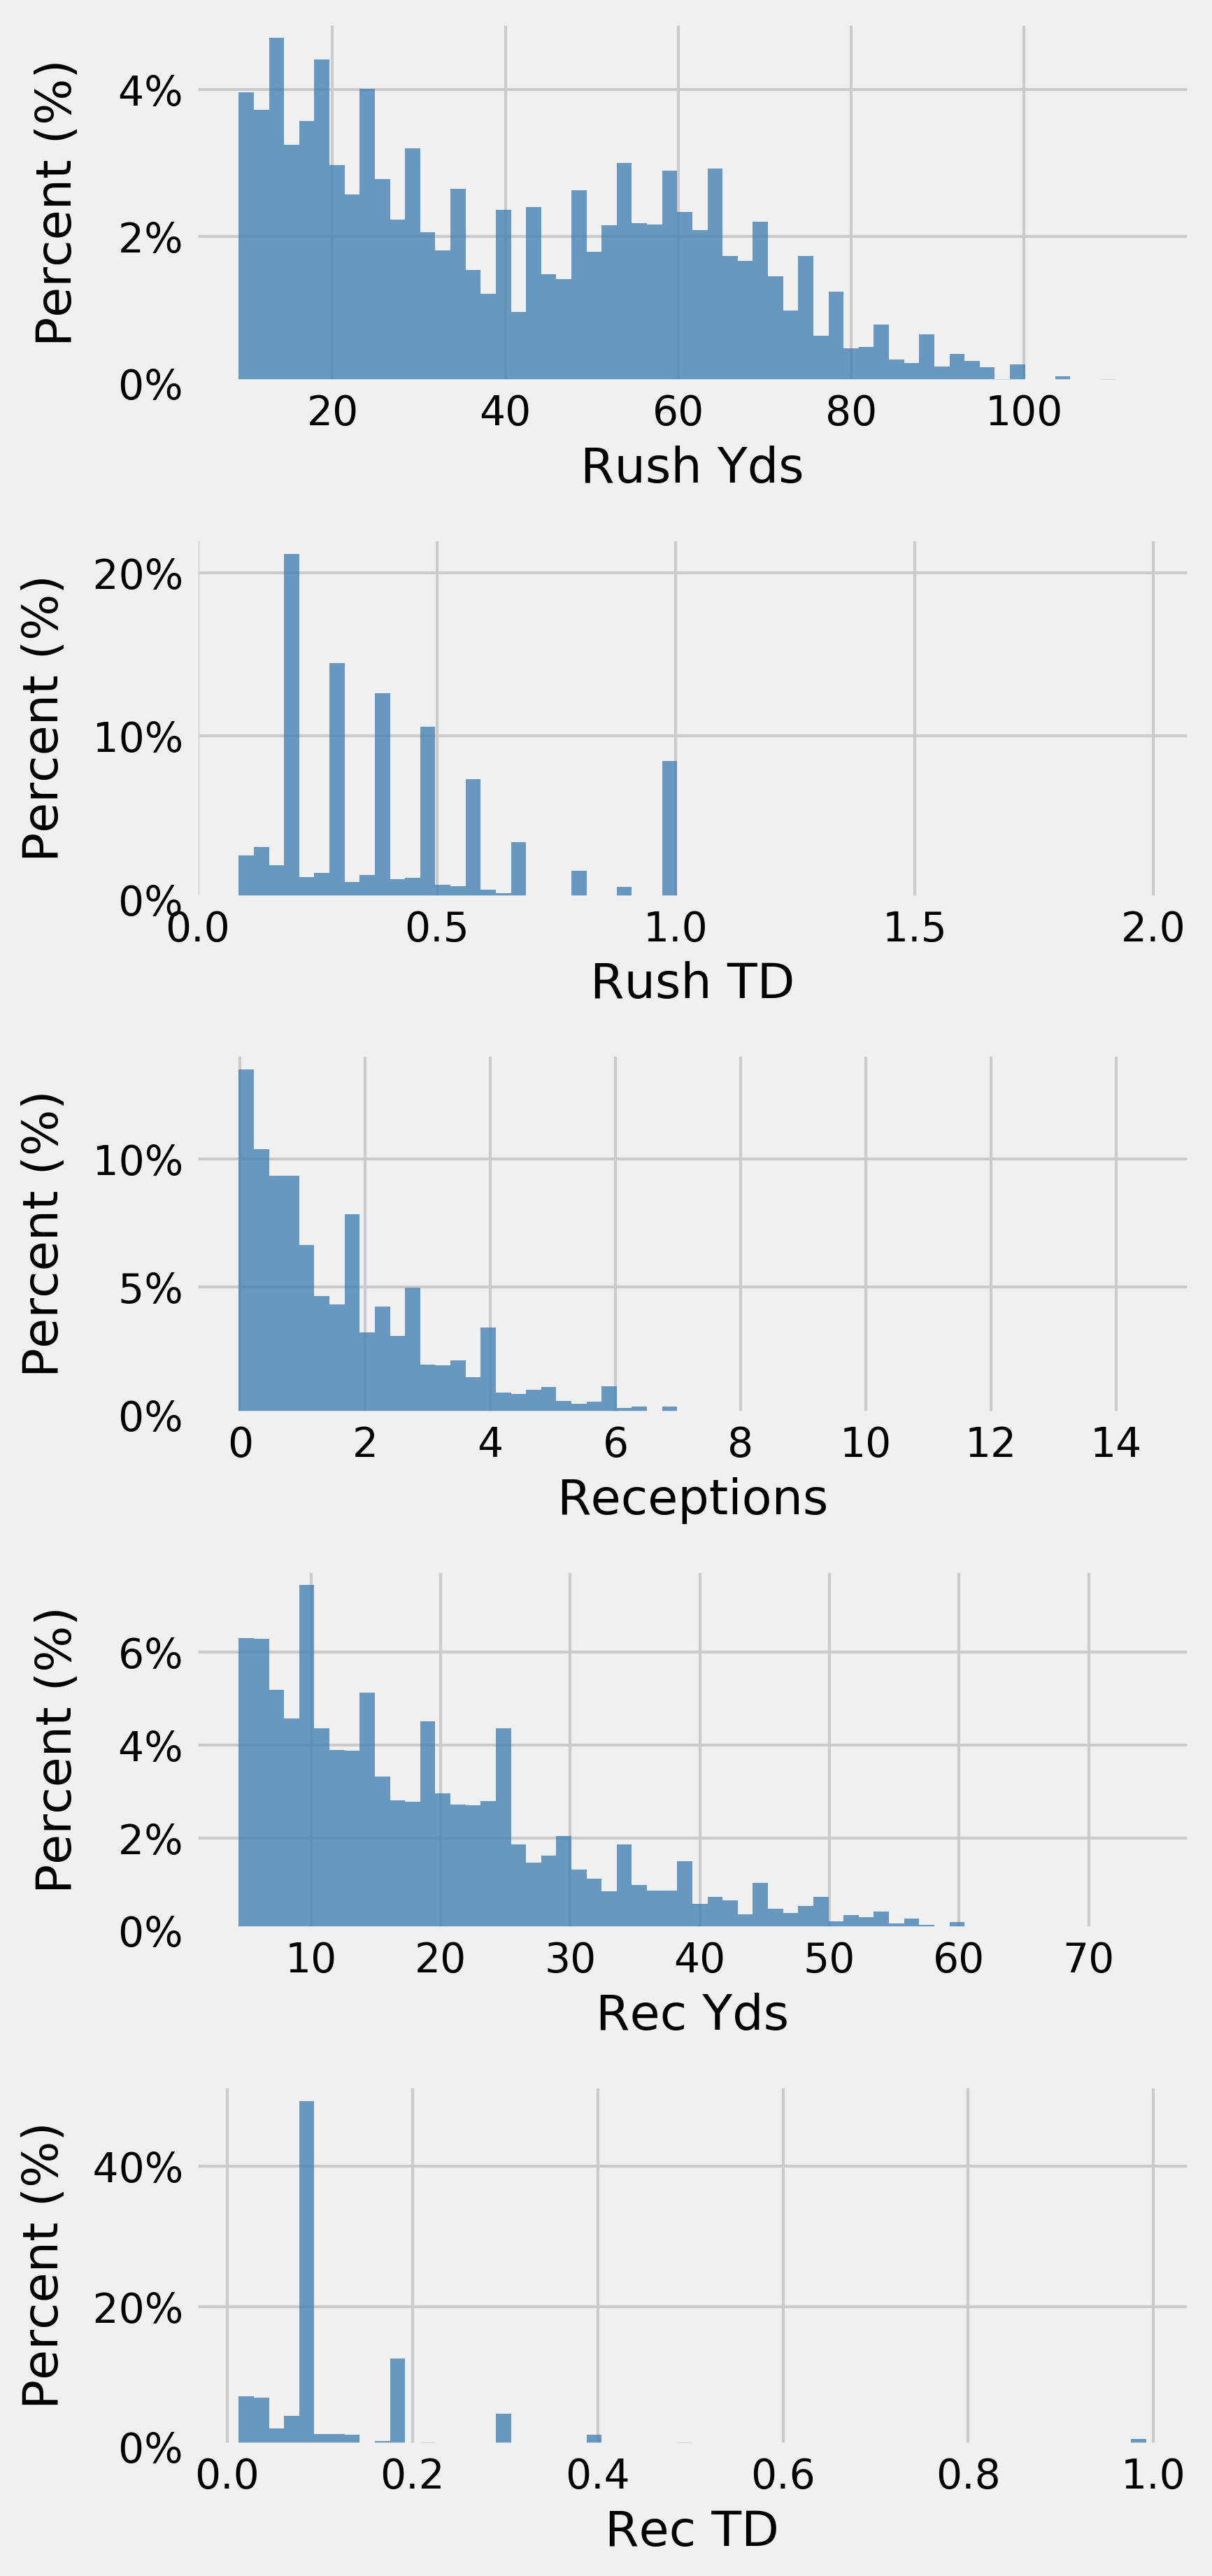
\includegraphics[width=1\textwidth]{../figures/threshold_hist_RB}
    \caption{Histogram above threshold.}
  \end{subfigure}
  \caption{Essential stat raw histograms and thresholded histograms for RB.}
\end{figure}

\pagebreak
\begin{figure}[H]
  \centering
  \begin{subfigure}[b]{0.450\textwidth}
    \centering
    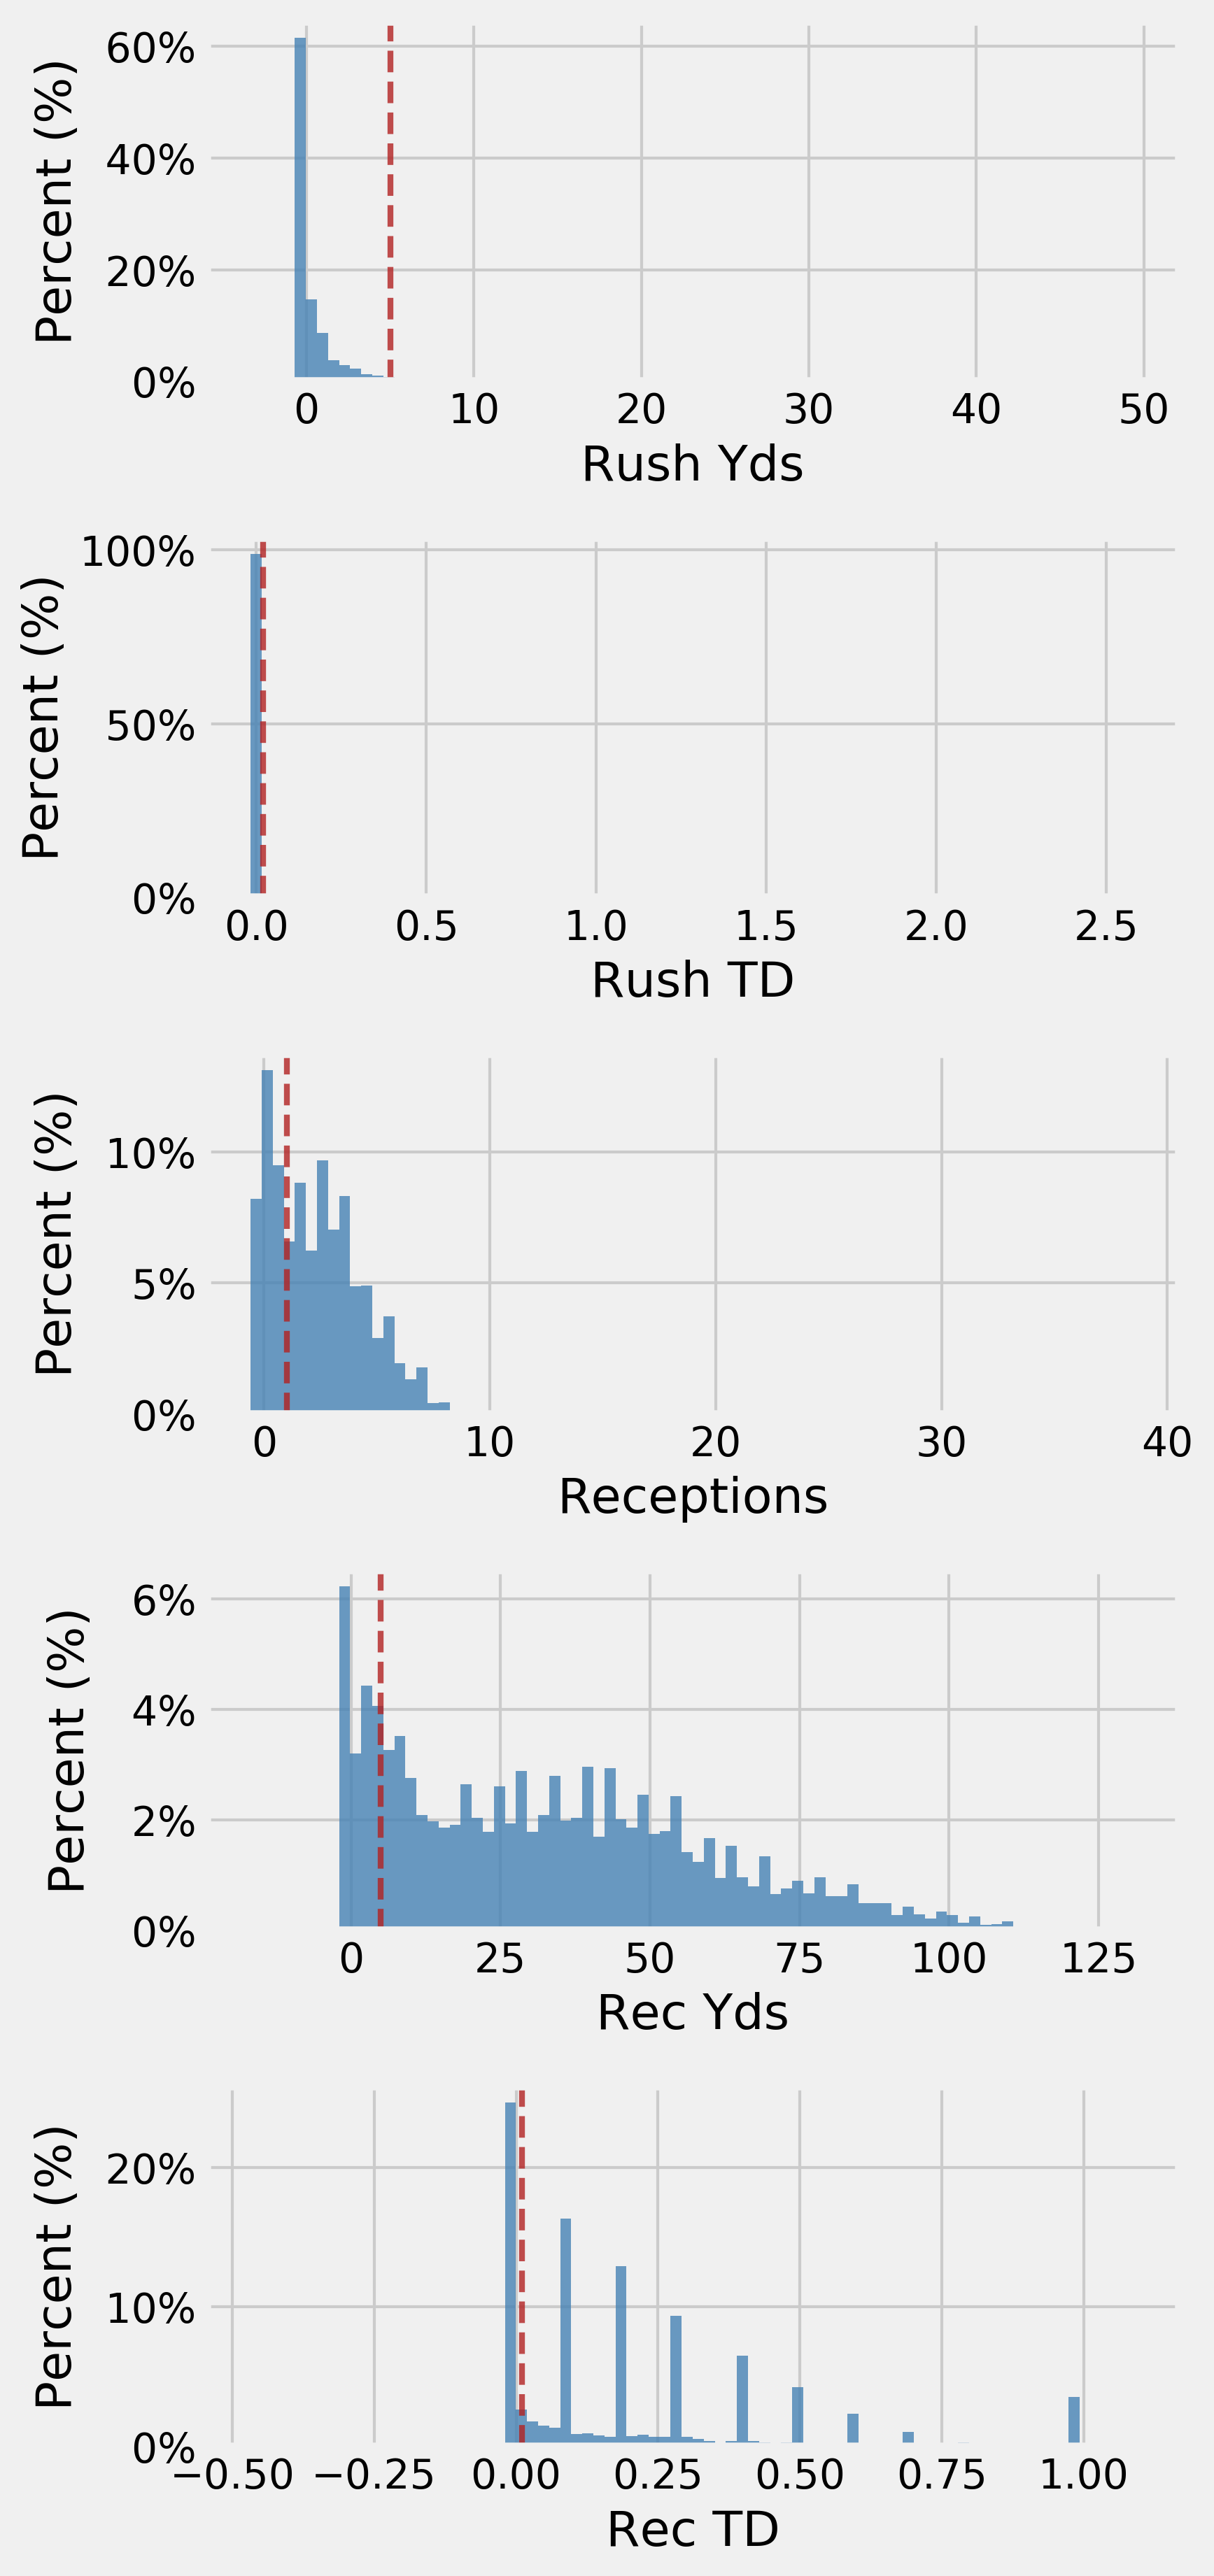
\includegraphics[width=1\textwidth]{../figures/no_threshold_hist_WR}
    \caption{Raw histogram with threshold (red).}
  \end{subfigure}
  \hfill
  \begin{subfigure}[b]{0.450\textwidth}
    \centering
    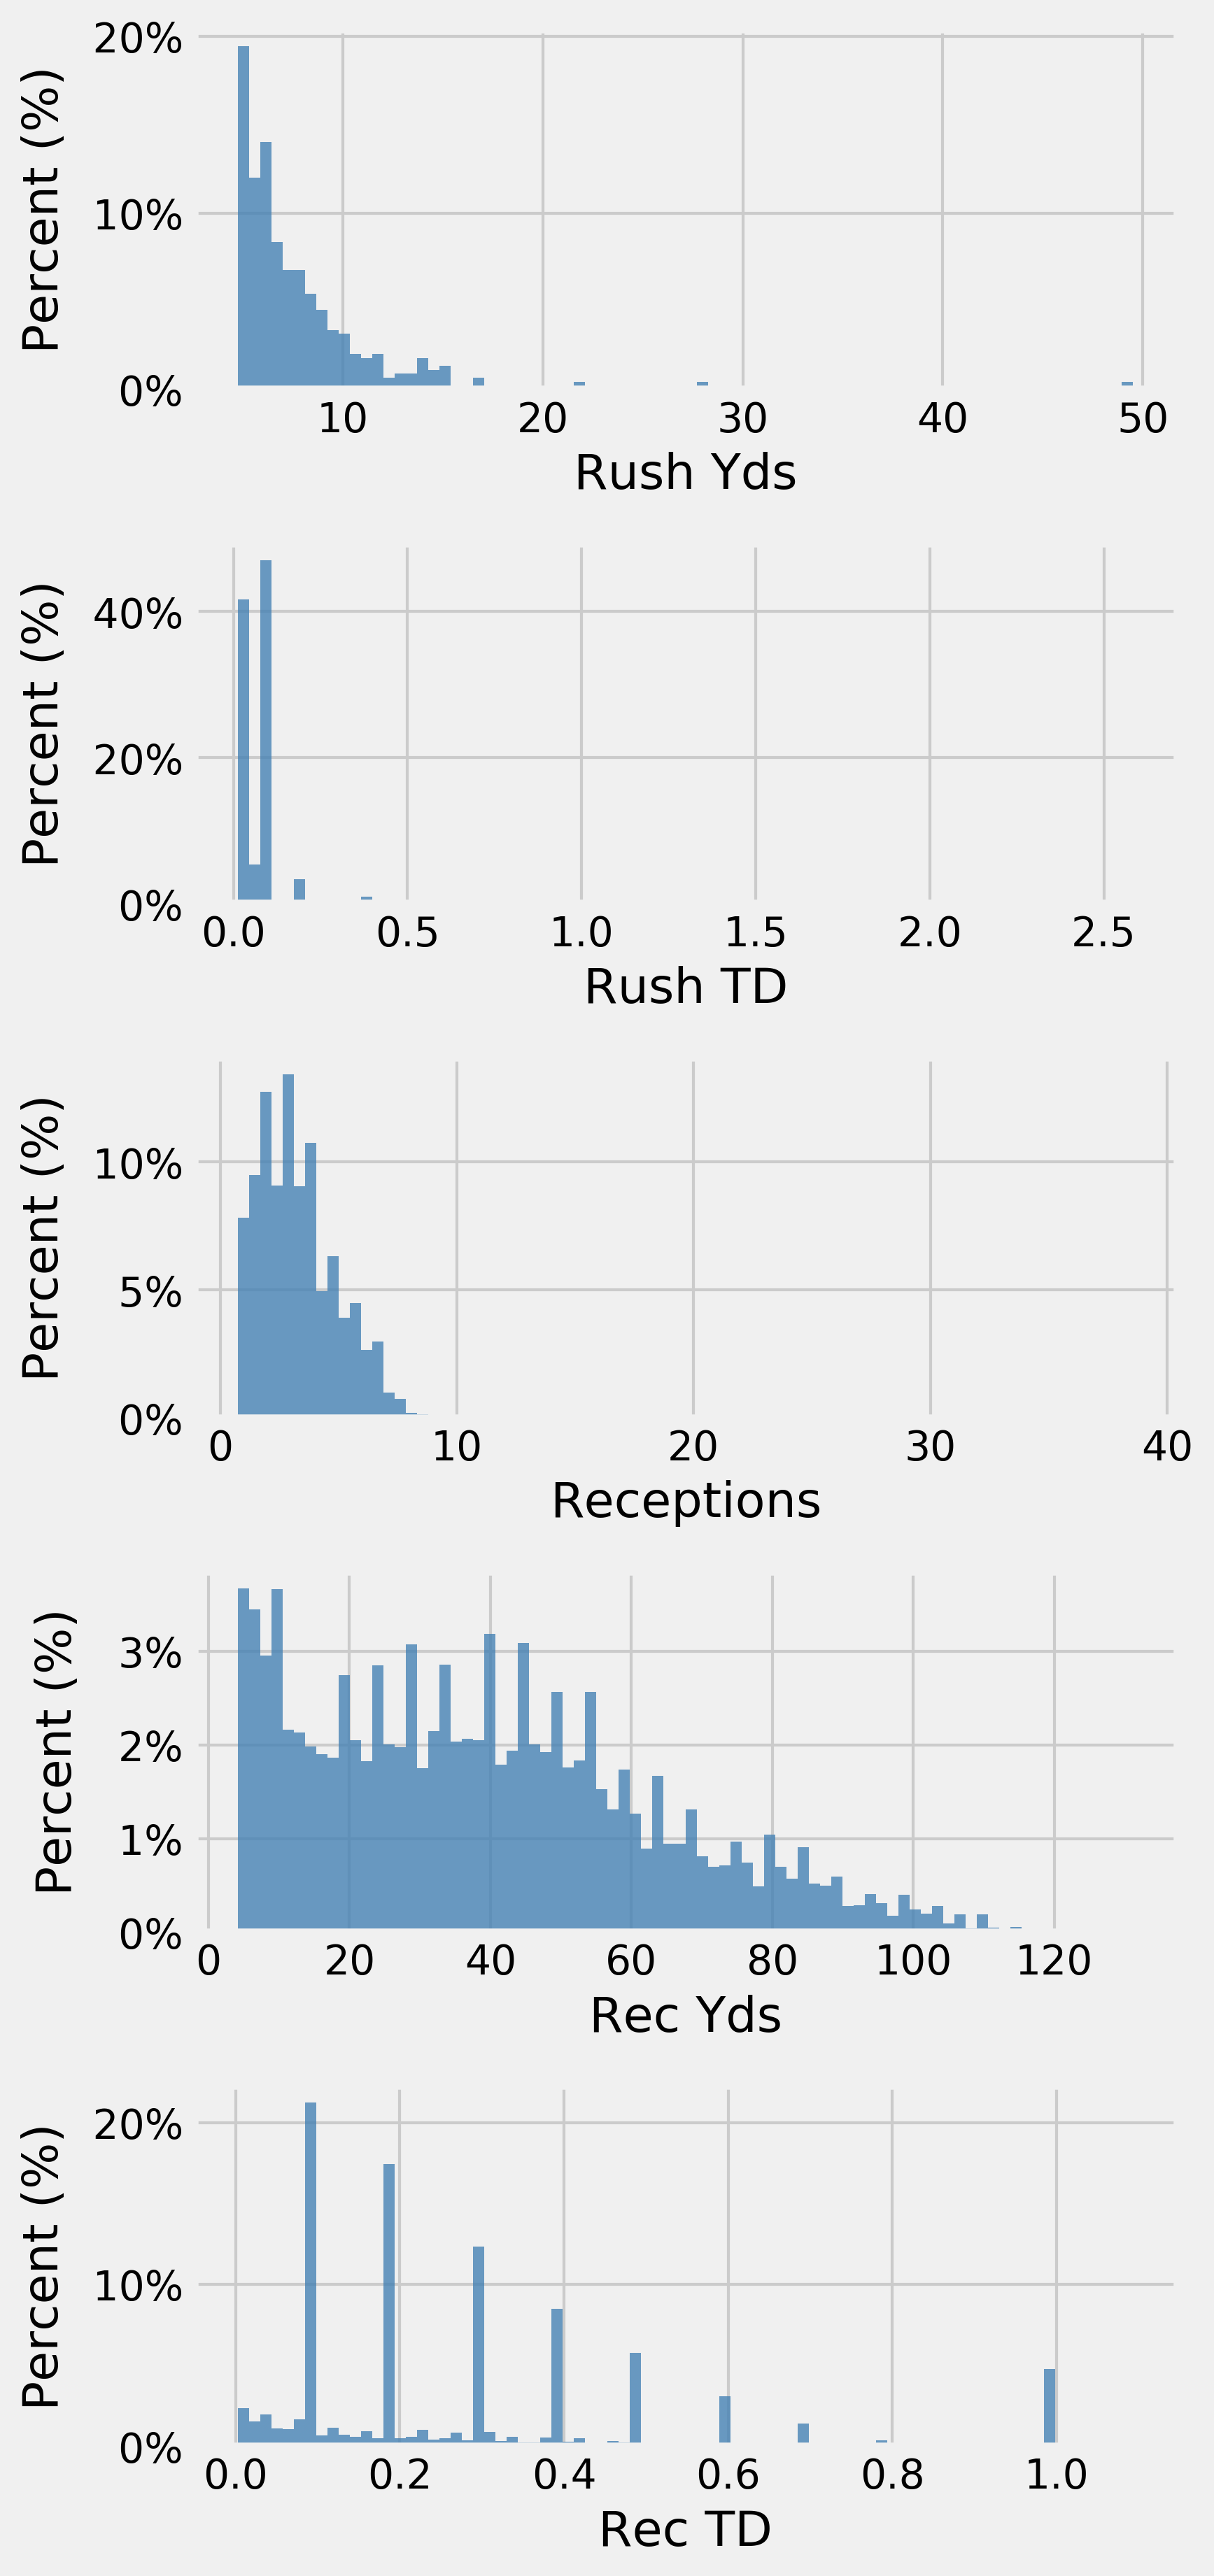
\includegraphics[width=1\textwidth]{../figures/threshold_hist_WR}
    \caption{Histogram above threshold.}
  \end{subfigure}
  \caption{Essential stat raw histograms and thresholded histograms for WR.}
\end{figure}

\pagebreak
\begin{figure}[H]
  \centering
  \begin{subfigure}[b]{0.450\textwidth}
    \centering
    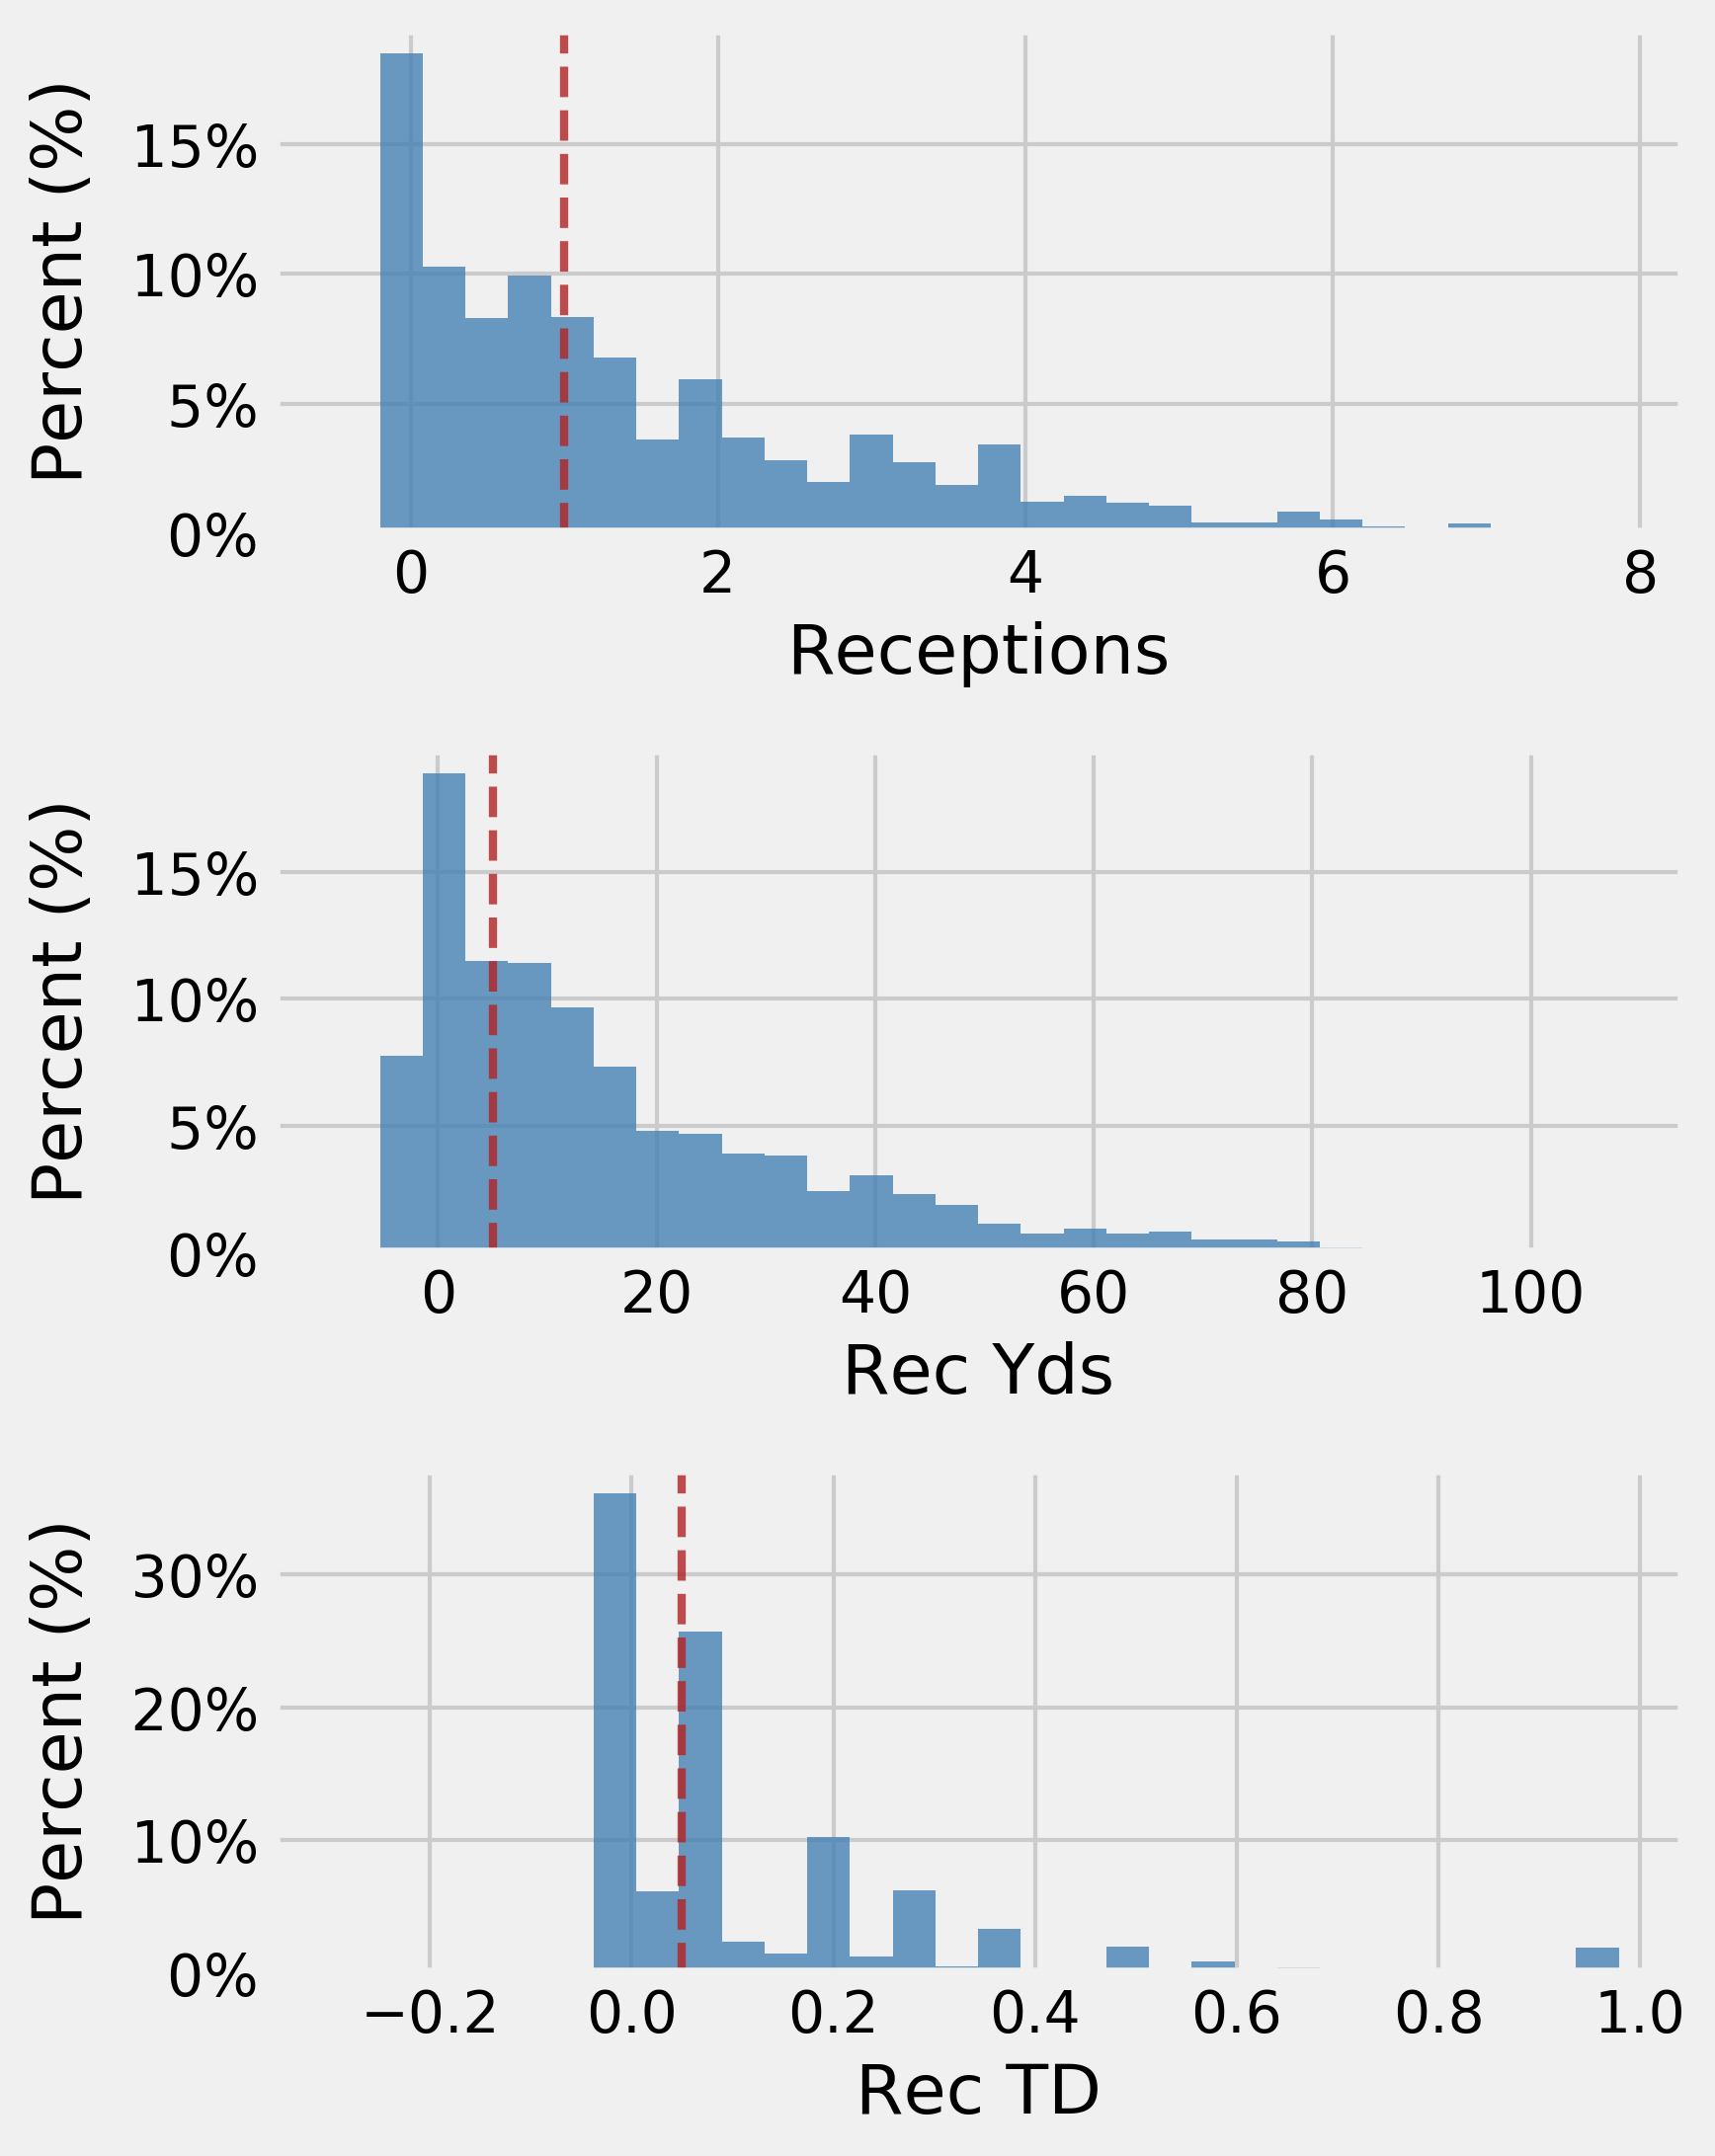
\includegraphics[width=1\textwidth]{../figures/no_threshold_hist_TE}
    \caption{Raw histogram with threshold (red).}
  \end{subfigure}
  \hfill
  \begin{subfigure}[b]{0.450\textwidth}
    \centering
    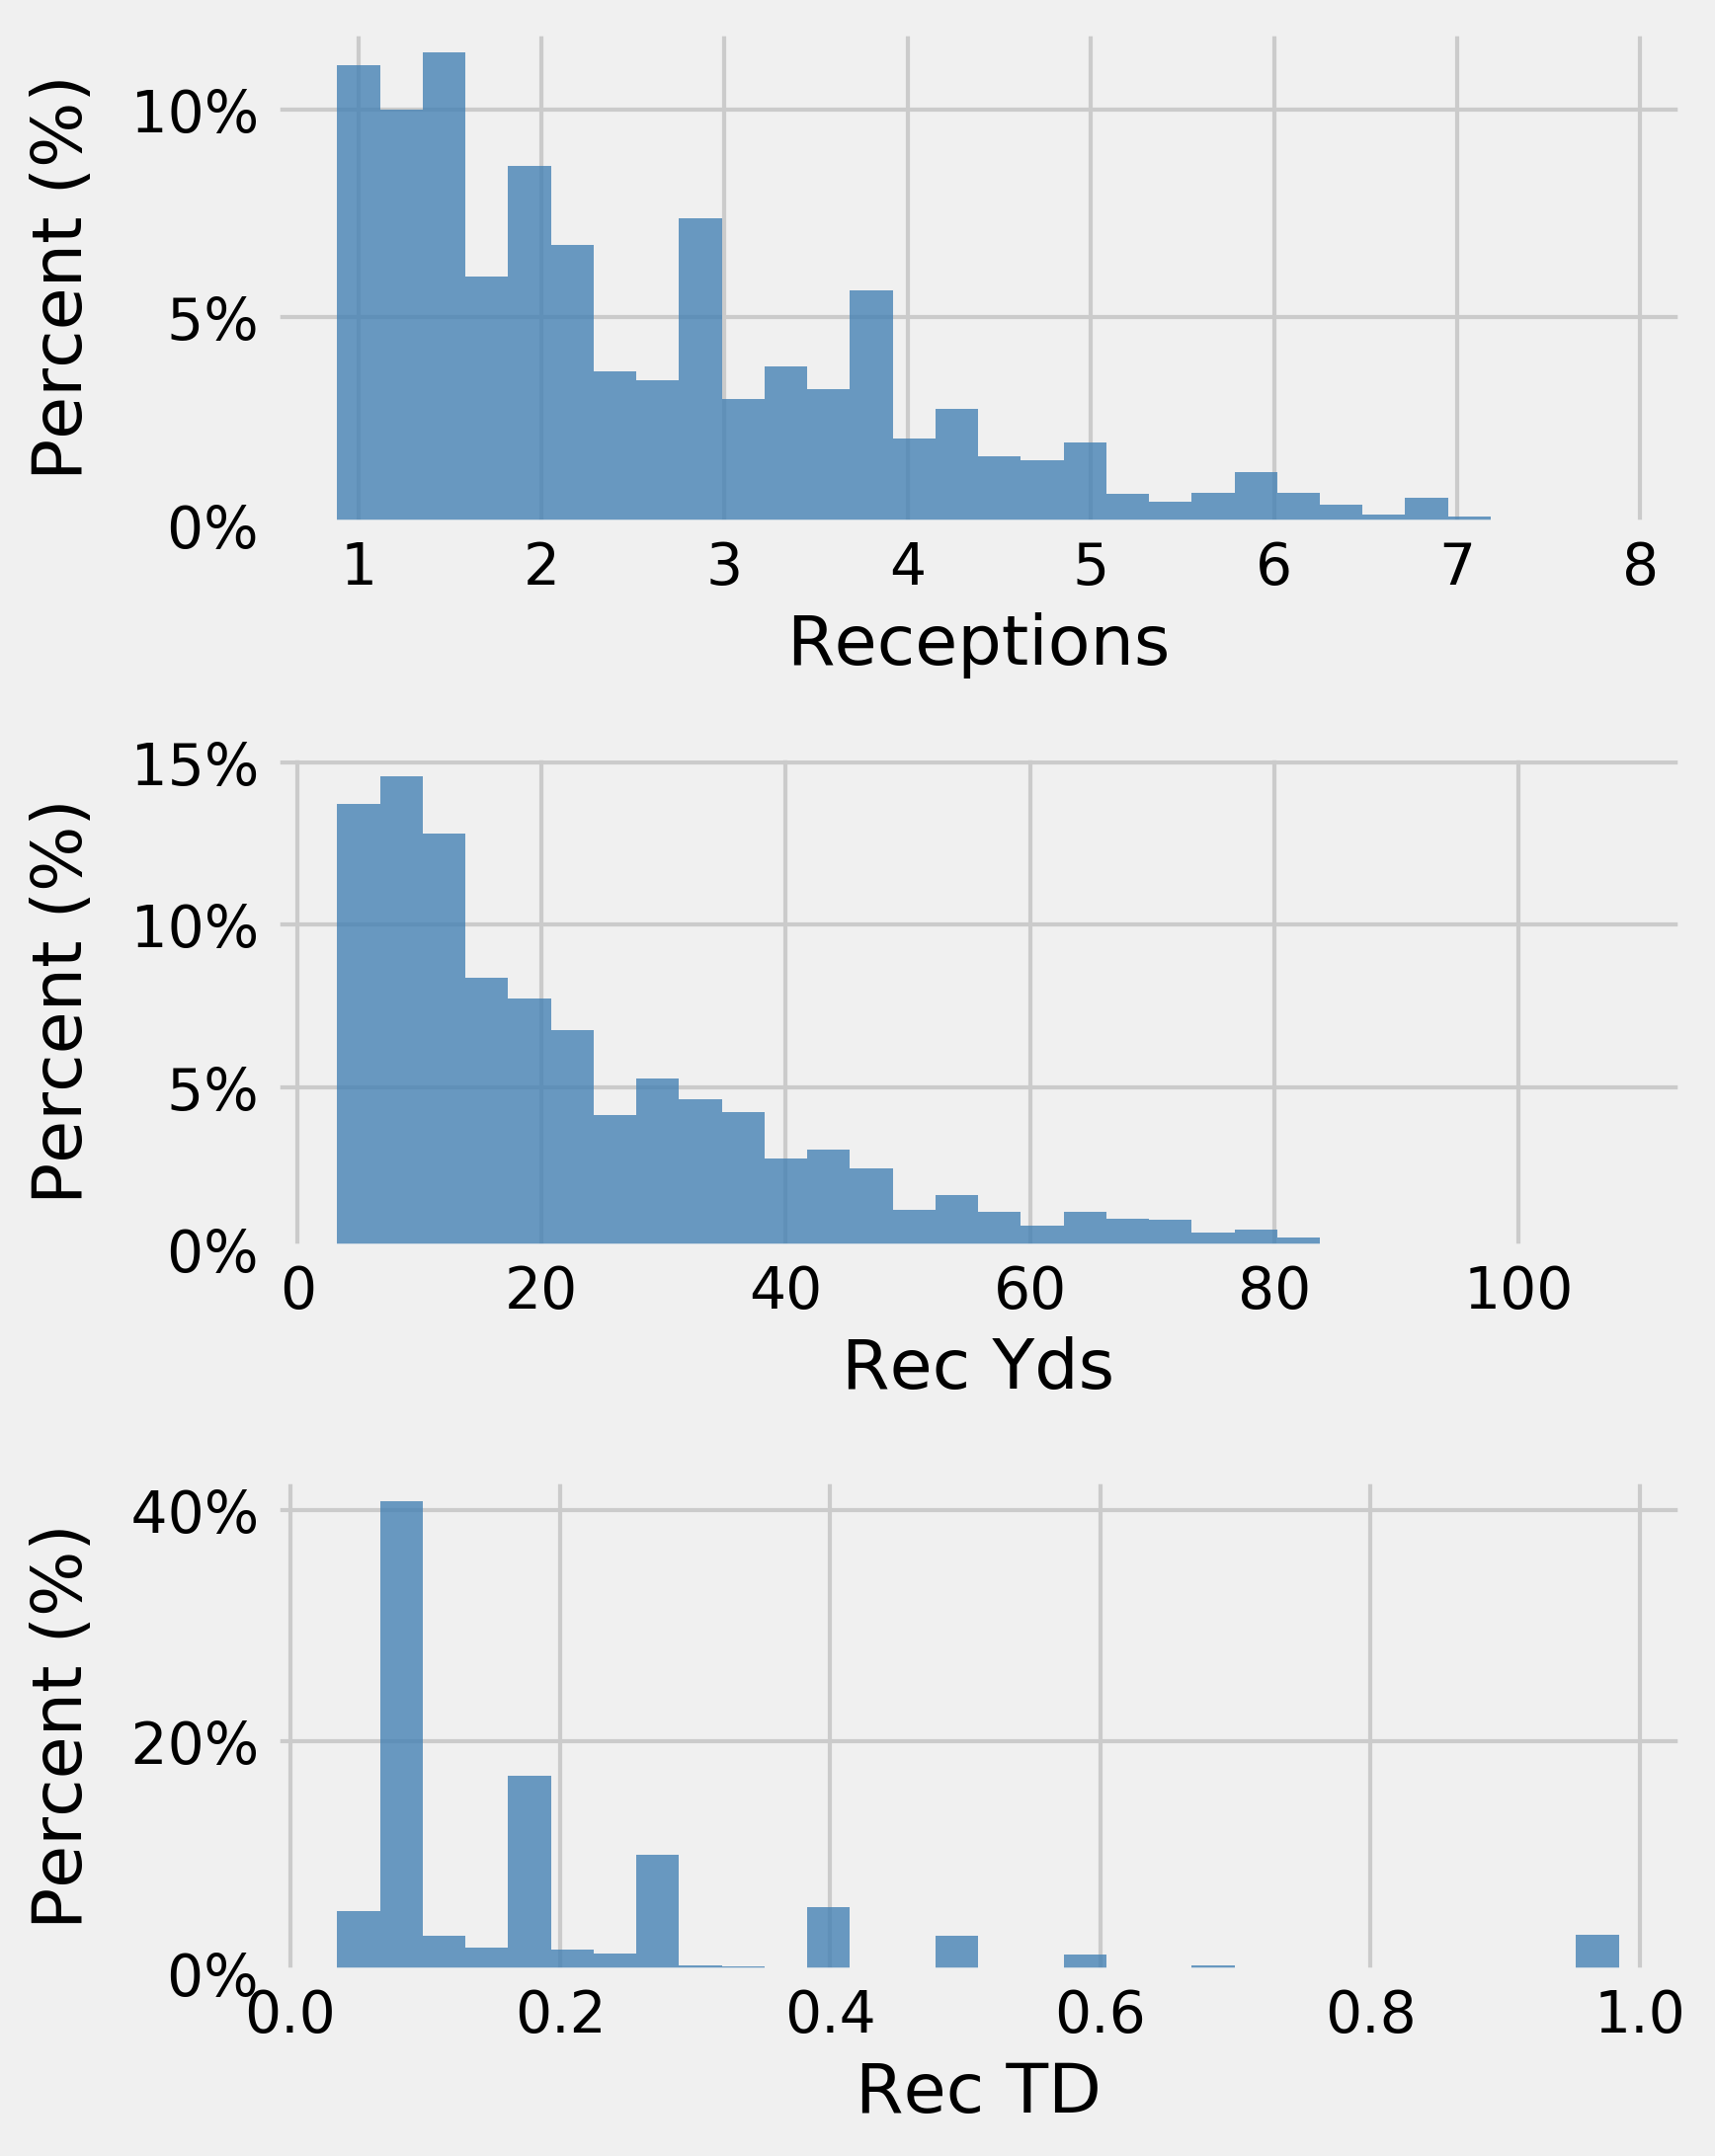
\includegraphics[width=1\textwidth]{../figures/threshold_hist_TE}
    \caption{Histogram above threshold.}
  \end{subfigure}
  \caption{Essential stat raw histograms and thresholded histograms for TE.}
\end{figure}

\pagebreak
\begin{figure}[H]
  \centering
  \begin{subfigure}[b]{0.450\textwidth}
    \centering
    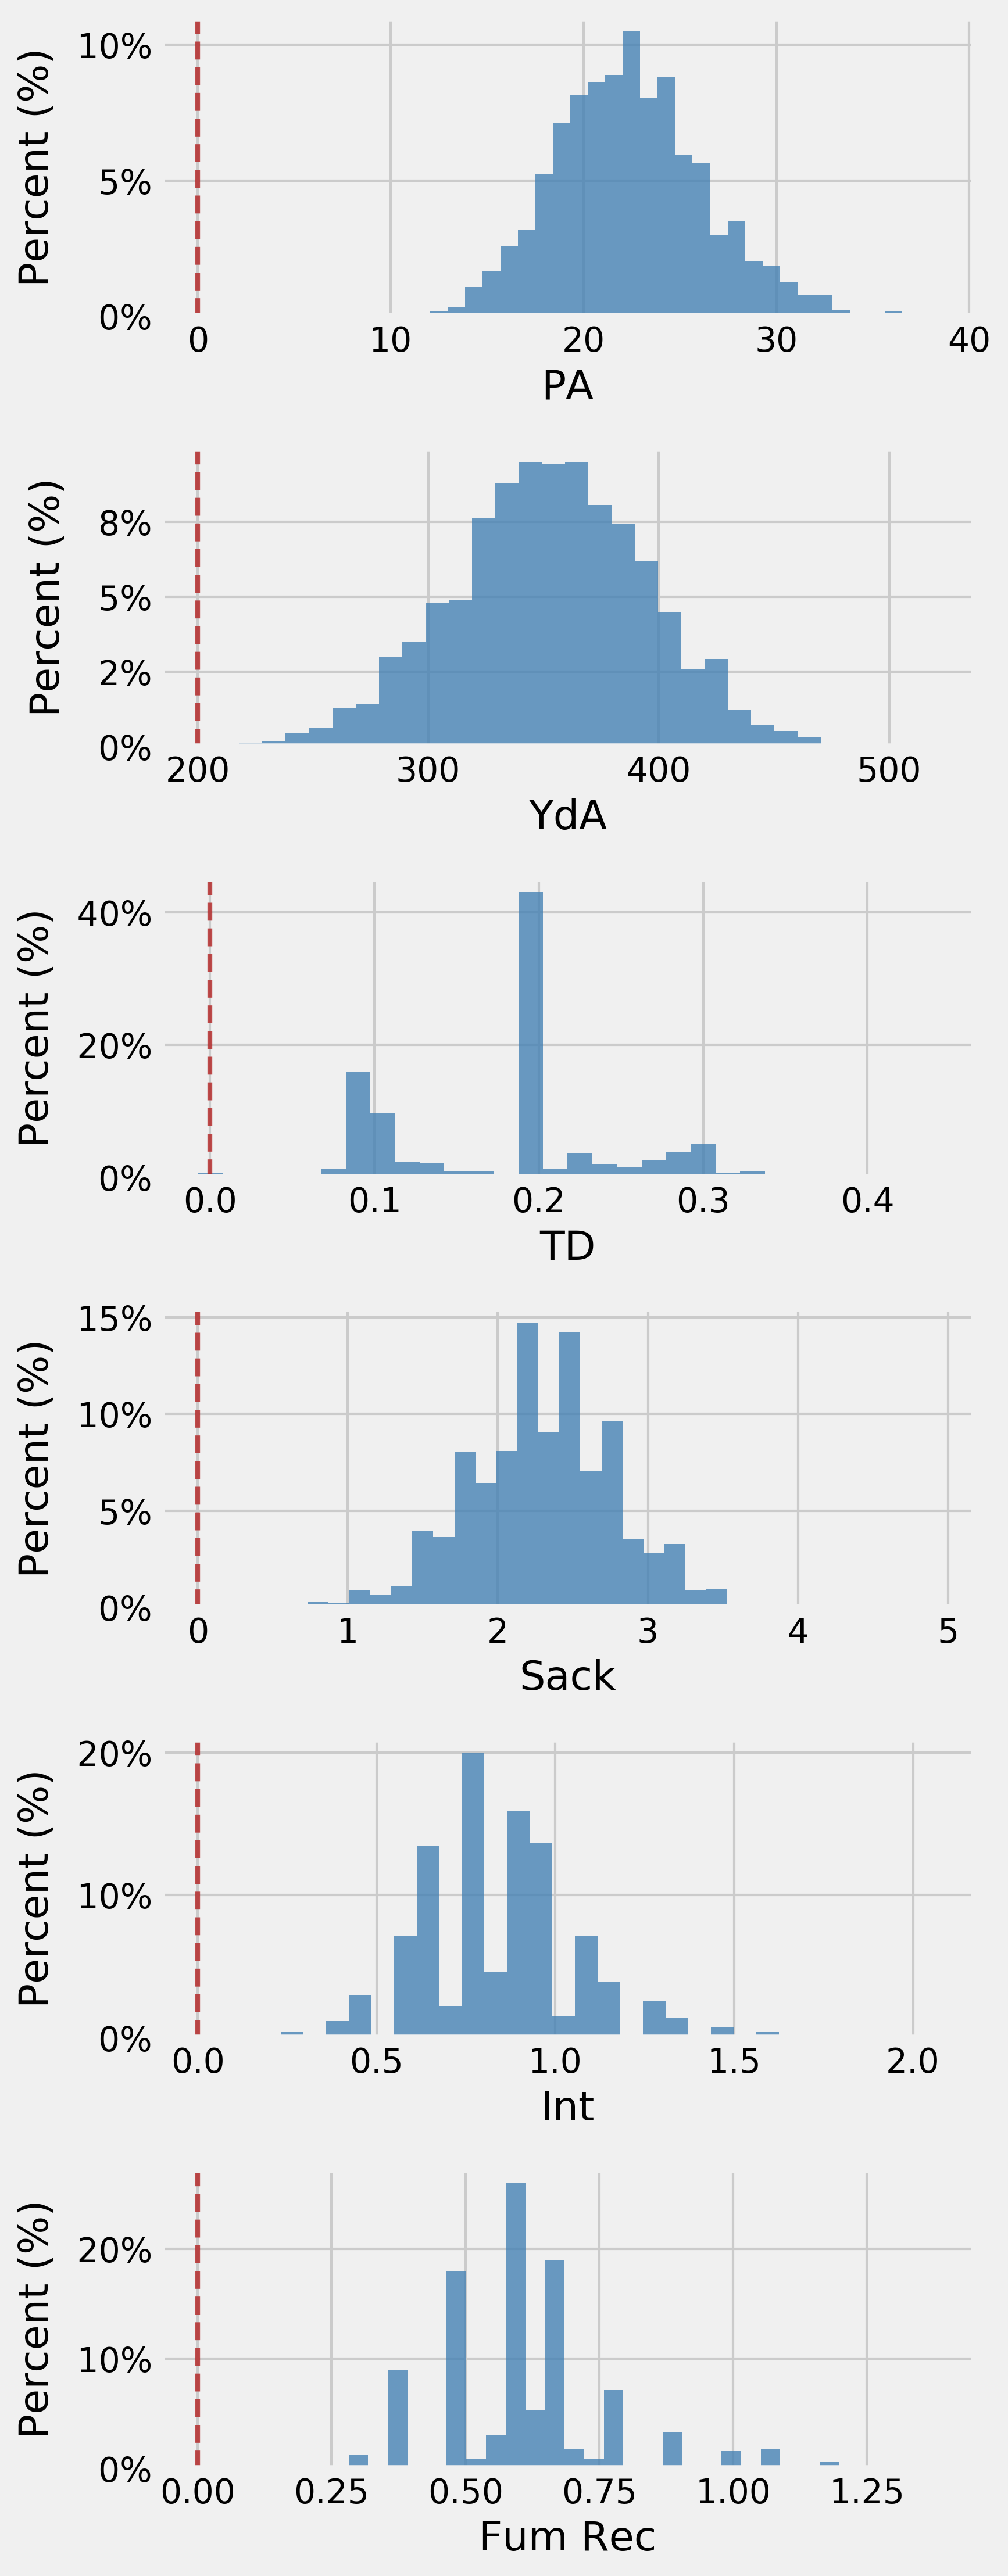
\includegraphics[width=1\textwidth]{../figures/no_threshold_hist_DST}
    \caption{Raw histogram with threshold (red).}
  \end{subfigure}
  \hfill
  \begin{subfigure}[b]{0.450\textwidth}
    \centering
    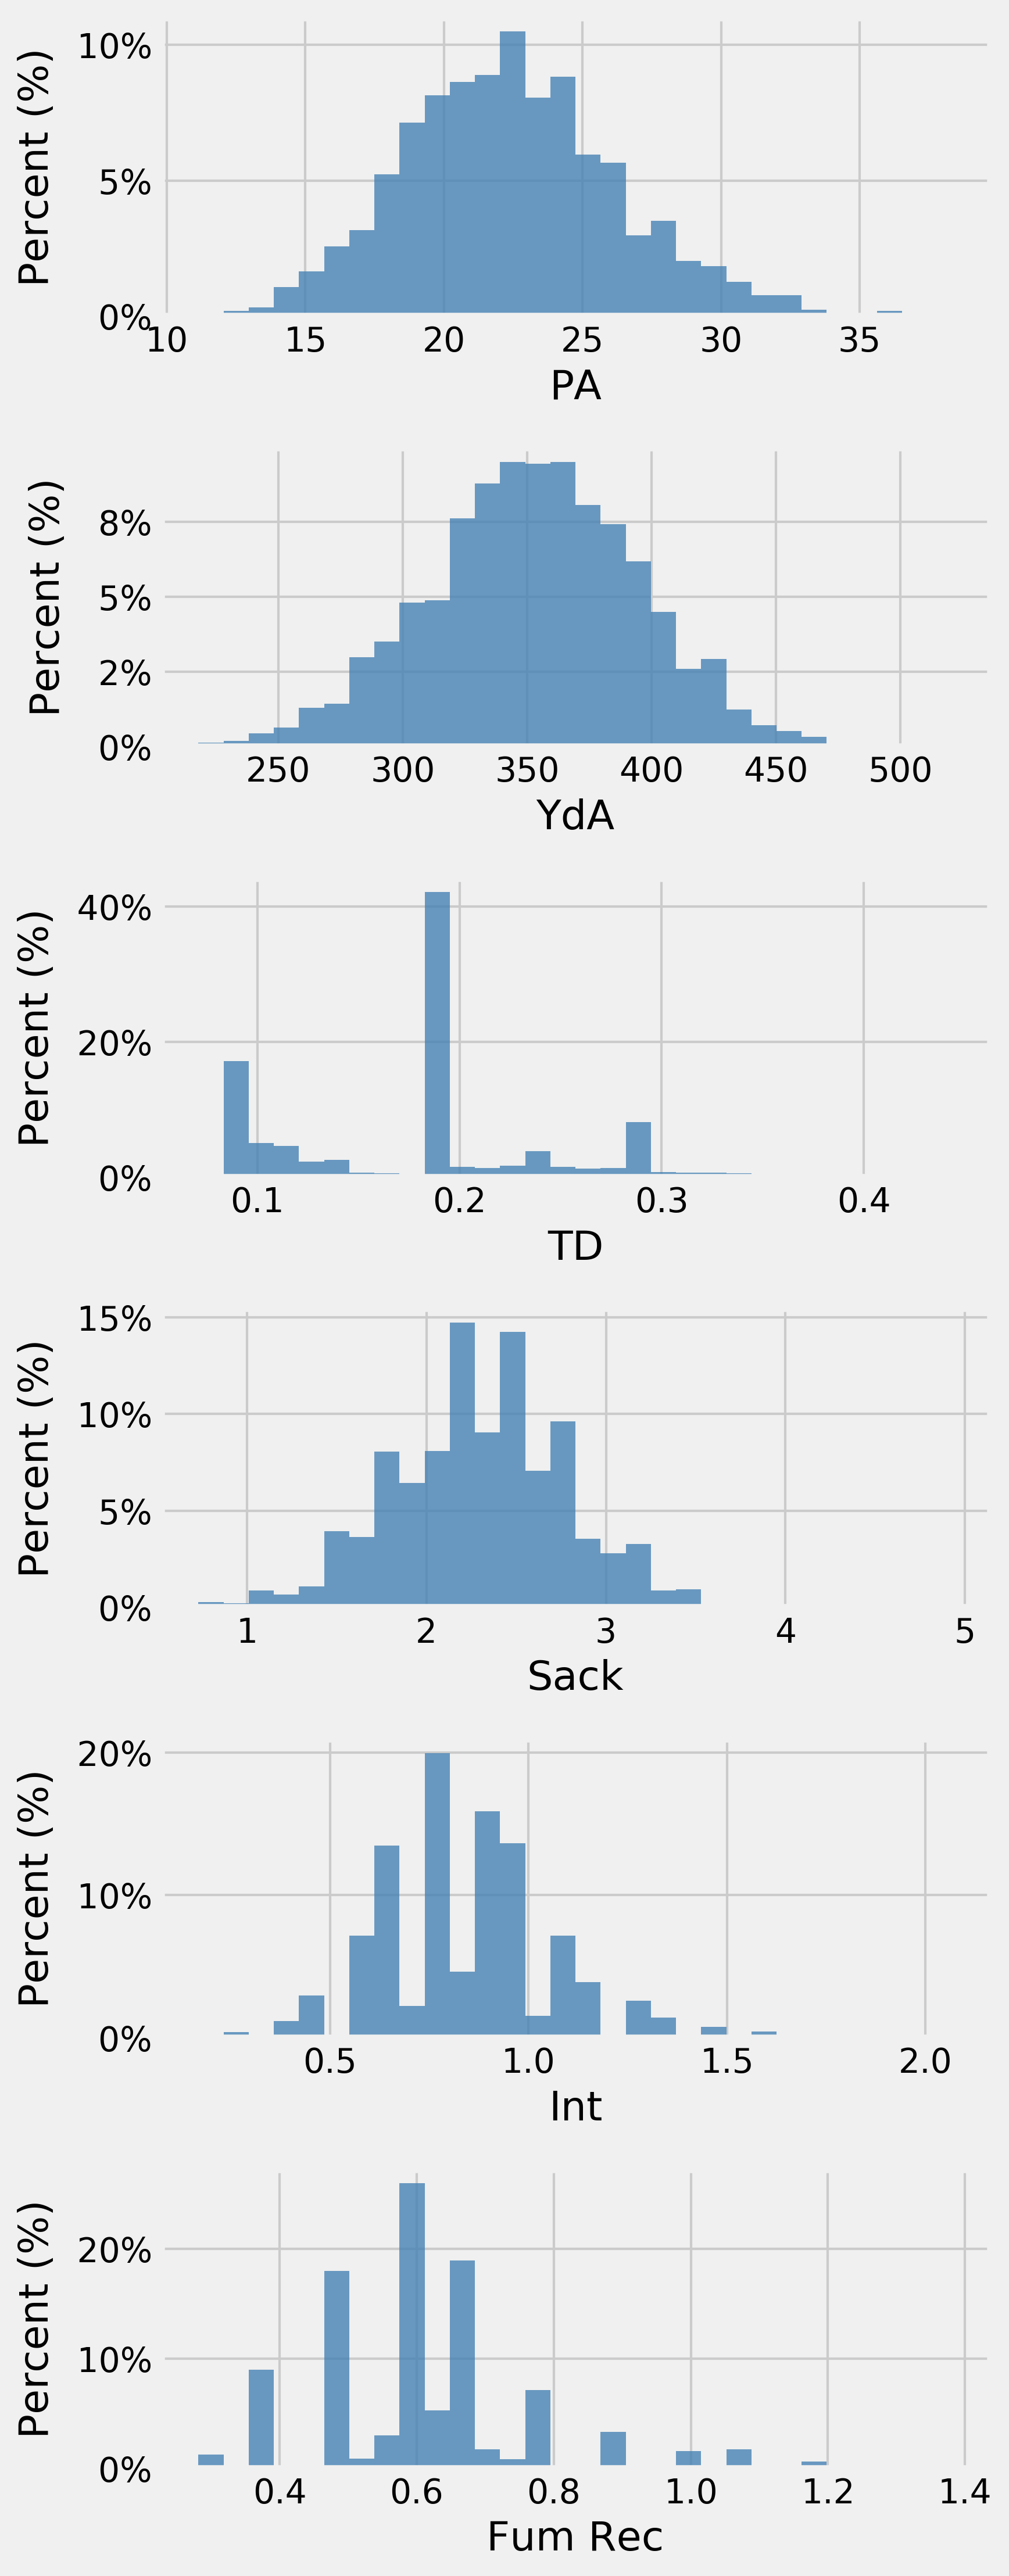
\includegraphics[width=1\textwidth]{../figures/threshold_hist_DST}
    \caption{Histogram above threshold.}
  \end{subfigure}
  \caption{Essential stat raw histograms and thresholded histograms for DST.}
\end{figure}

\pagebreak
\section{Ensemble Results}


\begin{table}[H]
\caption{Simple linear regression results for ensemble weighting of each source. Asterisks denote statistical significance of regression coefficients, (*) denoting a p-value less than 0.5, (**) for less than 0.01, and (***) for less than 0.001.}
\centering
\begin{adjustbox}{width =\textwidth}
\begin{tabular}{llllllllll}
\toprule
{} & Position &        Stat &    const &     ESPN &    Yahoo & FantasyPros &      NFL &      CBS &   FFToday \\
\midrule
{} &       QB &    Pass Yds &   -39.79 &     0.29 &     0.38 &       -0.44 &     0.26 &    -0.13 &     0.8** \\
{} &          &     Pass TD &    -0.08 &     0.19 &     0.05 &        0.62 &     -0.3 &     0.45 &      0.08 \\
{} &          &    Pass Int &    -0.05 &    -0.25 &     0.37 &        0.57 &     0.57 &     0.04 &     -0.28 \\
{} &          &    Rush Yds &  3.14*** &     0.12 &     0.01 &       -0.43 &     0.27 &     0.21 &    0.66** \\
{} &          &     Rush TD &     0.01 &     0.48 &    -0.16 &        0.38 &     0.77 &     -0.4 &     -0.17 \\
{} &       RB &    Rush Yds &     3.84 &  0.42*** &     0.25 &        0.17 &     0.25 &     0.01 &     -0.19 \\
{} &          &     Rush TD &     0.06 &    -0.05 &     0.14 &        0.56 &     0.29 &     0.23 &     -0.15 \\
{} &          &  Receptions &     0.08 &   0.3*** &   0.19** &        0.03 &     0.17 &     0.08 &   0.21*** \\
{} &          &     Rec Yds &     2.84 &  0.57*** &     0.11 &       -0.46 &     0.16 &     0.17 &   0.37*** \\
{} &          &      Rec TD &     0.04 &    -0.39 &     0.37 &        0.83 &   0.8*** &    -0.33 &  -0.33*** \\
{} &       WR &    Rush Yds &   25.03* &   1.54** &    -0.96 &       -2.82 &     0.31 &     0.32 &         - \\
{} &          &  Receptions &     0.22 &    0.44* &     0.08 &        -0.2 &   0.29** &  0.27*** &      0.06 \\
{} &          &     Rec Yds &     0.71 &   0.48** &      0.2 &        0.04 &     0.17 &    -0.04 &      0.14 \\
{} &          &      Rec TD &     0.03 &   0.56** &     0.03 &         0.5 &    -0.01 &     0.02 &     -0.11 \\
{} &       TE &  Receptions &  0.39*** &    -0.06 &     0.08 &        0.37 &   0.53** &    -0.16 &       0.1 \\
{} &          &     Rec Yds &     2.69 &    -0.06 &     0.05 &     0.93*** &    0.59* &    -0.27 &     -0.29 \\
{} &          &      Rec TD &   0.08** &  0.67*** &    -0.35 &       -0.34 &  0.71*** &    -0.12 &      0.14 \\
{} &      DST &          PA &     0.39 &        - &   0.8*** &        0.14 &    -0.29 &     0.33 &         - \\
{} &          &         YdA &    39.35 &        - &  0.36*** &        0.61 &        - &    -0.08 &         - \\
{} &          &          TD &    -0.25 &    -0.46 &     0.43 &       -0.26 &   3.38** &     0.26 &         - \\
{} &          &        Sack &    -0.26 &     0.06 &     0.34 &       -0.09 &     0.82 &     0.09 &         - \\
{} &          &         Int &    -0.27 &    -0.34 &     0.19 &        1.13 &     0.15 &      0.1 &         - \\
{} &          &     Fum Rec &     0.58 &     0.66 &    -0.45 &       -0.07 &     0.26 &    -0.31 &         - \\
\bottomrule
\end{tabular}
\end{adjustbox}
\end{table}






\end{document}
